%!TEX encoding = UTF-8 Unicode
% ================================================================================
\documentclass[
	fontsize=11pt,
	headings=small,
	parskip=half,           % Ersetzt manuelles Setzen von parskip/parindent.
	bibliography=totoc,
	numbers=noenddot,       % Entfernt den letzten Punkt der Kapitelnummern.
	open=any,               % Kapitel kann auf jeder Seite beginnen.
%	final                   % Entfernt alle todonotes und den Entwurfstempel.
]{scrreprt}
% ================================================================================
%!TEX encoding = UTF-8 Unicode
%!TEX root = hinweiseabschlussarbeit.tex

% Kodierung, Sprache, Patches {{{
\usepackage[T1]{fontenc}    % Ausgabekodierung; ermöglicht Akzente und Umlaute
                            %  sowie korrekte Silbentrennung.
%\usepackage[utf8]{inputenc} % Erlaubt die direkte Eingabe spezieller Zeichen;
                            %  utf8 muss die Eingabekodierung des Editors sein.
\usepackage[ngerman]{babel} % Deutsche Sprachanpassungen (z.B. Überschriften).
\usepackage{microtype}      % Optimale Randausrichtung und Skalierung.
\usepackage[
    autostyle,
    ]{csquotes}             % Korrekte Anführungszeichen in der Literaturliste.
%\usepackage{fixltx2e}      % Patches fuer LaTeX2e - seit 2015 nicht mehr nötig
\usepackage{scrhack}        % Verhindert Warnungen mit älteren Paketen.
\usepackage[
  newcommands
]{ragged2e}                 % Verbesserte \ragged...Befehle
\PassOptionsToPackage{
  hyphens
}{url}                      % Sorgt für URL-Umbrüche in Fußzeilen u. Literatur
% }}}

% Schriftarten {{{
\usepackage{mathptmx}       % Times; modifies the default serif and math fonts
\usepackage[scaled=.92]{helvet}% modifies the sans serif font
\usepackage{courier}        % modifies the monospace font
% }}}

% Biblatex {{{
\usepackage[
    style=alphabetic,
    backend=biber,
    %backref=true
    ]{biblatex}             % Biblatex mit alphabetischem Style und biber.
\bibliography{\jobname.bib} % Dateiname der bib-Datei.
\DeclareFieldFormat*{title}{
    \mkbibemph{#1}}         % Make titles italics
% }}}

% Dokument- und Texteinstellungen {{{
\usepackage[
    a4paper,
    margin=2.54cm,
    marginparwidth=2.0cm,
    footskip=1.0cm
    ]{geometry}             % Ersetzt 'a4wide'.
\clubpenalty=10000          % Keine Einzelzeile am Beginn eines Absatzes
                            %  (Schusterjungen).
\widowpenalty=10000         % Keine Einzelzeile am Ende eines Absatzes
\displaywidowpenalty=10000  %  (Hurenkinder).
\usepackage{floatrow}       % Zentriert alle Floats
\usepackage{ifdraft}        % Ermöglicht \ifoptionfinal{true}{false}
\pagestyle{plain}           % keine Kopfzeilen
% \sloppy                    % großzügige Formatierungsweise
\deffootnote{1em}{1em}{
  \thefootnotemark.\ }      % Verbessert Layout mehrzeiliger Fußnoten
\ifdefined\chapterformat
	\renewcommand*{\chapterformat}{% Hübscht Kapitelüberschrift mit senkrechtem 
		\thechapter\enskip%          grauen Balken zwischen Nummer und Text auf
		\textcolor{gray!50}{\rule[-\dp\strutbox]{2pt}{\baselineskip}}\enskip
	}
\fi
%\setkomafont{disposition}{\normalcolor\bfseries} % Aus der KOMA-Skript-Anleitung: „Mit dieser Änderung verzichten Sie darauf, für alle Gliederungsebenen serifenlose Schrift voreinzustellen“

\makeatletter
\AtBeginDocument{%
    \hypersetup{%
        pdftitle = {\@title},
        pdfauthor  = \@author,
    }
}
\makeatother
% }}}

% Weitere Pakete {{{
\usepackage{graphicx}       % Einfügen von Graphiken.
\usepackage{tabu}           % Einfügen von Tabellen.
\usepackage{multirow}       % Tabellenzeilen zusammenfassen.
\usepackage{multicol}       % Tabellenspalten zusammenfassen.
\usepackage{booktabs}       % Schönere Tabellen (\toprule\midrule\bottomrule).
\usepackage[nocut]{thmbox}  % Theorembox bspw. für Angreifermodell.
\usepackage{amsmath}        % Erweiterte Handhabung mathematischer Formeln.
\usepackage{amssymb}        % Erweiterte mathematische Symbole.
\usepackage{rotating}
\usepackage[
    printonlyused
    ]{acronym}              % Abkürzungsverzeichnis
\usepackage[
    colorinlistoftodos,
    textsize=tiny,          % Notizen und TODOs - mit der todonotes.sty von
    \ifoptionfinal{disable}{}%  Benjamin Kellermann ist das Package "changebar"
    ]{todonotes}            %  bereits integriert.
\usepackage[
    breaklinks,
    hidelinks,
    pdfdisplaydoctitle,
    pdfpagemode = {UseOutlines},
    pdfpagelabels,
    ]{hyperref}             % Sprungmarken im PDF. Lädt das URL-Paket.
    \urlstyle{rm}           % Entfernt die Formattierung von URLs.
%\usepackage{breakurl}
%\def\UrlBreaks{\do\/\do-}
\usepackage{listings}       % Spezielle Umgebung für Quelltextformatierung.
    \lstset{                
        language=C,
        breaklines=true,
        breakatwhitespace=true,
        frame=l,            % Linie links: l, doppelt: L
		framerule=2.5pt,    % Dicke der Linie
		rulecolor=\color{gray},% Farbe der Linie
        captionpos=b,
        xleftmargin=6ex,
        tabsize=4,
        numbers=left,
        numberstyle=\ttfamily\footnotesize,
        basicstyle=\ttfamily\footnotesize,
        keywordstyle=\bfseries\color{green!50!black},
        commentstyle=\itshape\color{magenta!90!black},
        identifierstyle=\ttfamily,
        stringstyle=\color{orange!90!black},
        showstringspaces=false,
        }
%\usepackage{filecontents}  % Direktes Einfügen von Dateiinhalt. Wird hier für
                            %  die Verwendung einer .bib-Datei in dieser .tex-
                            %  Datei benötigt.
% }}}
% \usepackage{parskip}

% \usepackage[pdftex]{graphicx}

\usepackage{colortbl}
\usepackage{xcolor}
\usepackage{soul}

\definecolor{uhhred}{cmyk}{0,100,100,0}
\addbibresource{main.bib}

\begin{document}

\title{Privatsphärewahrendes Anreiz- und Betrugserkennungssystem im\\ Datentreuhandmodell}
\author{Knut Hoffmeister}

\newgeometry{centering,left=2cm,right=2cm,top=2cm,bottom=2cm}
\begin{titlepage}

\includegraphics[width=6.8cm]{up-uhh-logo-u-2010-u-farbe-u-rgb.pdf}
\begin{center}
    \vfill
    \Large Bachelorarbeit
    \vfill
    \makeatletter
    {\Large\textsf{\textbf{\@title}}}
    \makeatother
    \vfill
    vorgelegt von
    \par\bigskip
    \makeatletter
    {\@author}
    \makeatother
    \par
    Matrikelnummer 7509085 \par
    Studiengang Software System Entwicklung
    \vfill
    MIN-Fakultät \par
    Fachbereich Informatik
    \vfill
    \makeatletter
    eingereicht am {\@date}
    \makeatother
    \vfill
    Erstgutachter: Prof. Dr.-Ing. Mathias Fischer\\
    Zweitgutachter: Kevin Röbert, M. Sc.
\end{center}
\ifoptionfinal{}{
    \begin{tikzpicture}[remember picture, overlay]
        \node[draw, red, font=\ttfamily\bfseries\Large, xshift=30mm, yshift=238mm, rotate=340, text centered, text width=6cm, very thick, rounded corners=4mm] at (current page.south) {Entwurf vom \today};
    \end{tikzpicture}
}
\end{titlepage}

\restoregeometry

\tableofcontents

\newgeometry{margin=1.5in}
\chapter*{Abstract}
In dieser Bachelorarbeit wird ein Bezahlsystem für die Verwendung in einem Datentreuhandmodell entworfen, welches zwei Maßnahmen für den Schutz vor Missbrauch liefert. In einem Datentreuhandmodell gibt es drei Akteure: Den Datentreuhänder, der als neutrale Instanz die Kommunikation verwaltet, den Datengebenden, der jegliche Form an Daten beim Datentreuhänder hochladen und lagern kann und den Datennutzenden, der an der kommerziellen oder wissenschaftlichen Auswertung der Daten interessiert ist. Das Bezahlsystem dient dazu, einen Anreiz für Datengebende zu schaffen, ihre Daten mit Datennutzenden zu teilen. Dafür wird ein Coin eingeführt, der von einem Exchange signiert und eingelöst werden kann. Der Coin kann als Gegenleistung im Tausch für Daten übertragen werden.

Die erste Maßnahme zum Schutz vor Missbrauch ist ein Streitfallsystem. Es erlaubt beiden am Handel beteiligten Parteien einen Streit auszurufen, sollten sie sich durch den Handel betrogen fühlen. Daraufhin werden die zuvor verschlüsselten Nachrichten für den Datentreuhänder einsehbar und er kann als neutrale Partei entscheiden, ob ein Betrug vorliegt.

Der zweite Schutzmechanismus ist ein Reputationssystem, dass jedem Datengebenden einen Ruf zuweist. Dieser Ruf setzt sich aus vergangenen Bewertungen von Datennutzenden zusammen, die die Qualität der gehandelten Daten bewerten. Betrügerische Datengebende können durch den Rufwert identifiziert und von Datennutzenden gemieden werden. 

Anforderungen an die entworfenen Systeme sind hauptsächlich die Anonymität des Datengebenden und die vertrauliche Kommunikation von Daten, sodass selbst der Datentreuhänder -- außer im Streitfall -- den Nachrichtenverkehr nicht zuordnen kann. Später werden die Systeme auf ihre Sicherheit gegen verschiedene Angreifer und auf ihr Laufzeitverhalten mit unterschiedlichen Parametern untersucht.

\restoregeometry
\chapter*{Abkürzungen und Notation}
\section*{Abkürzungen}
Im Rahmen dieser Bachelorarbeit wurden die folgenden Begriffe aufgrund der Frequenz ihrer Benutzung abgekürzt. Andere Begriffe oder Protokolle sind besser unter ihren Abkürzungen bekannt, weshalb diese hier statt dem ausgeschriebenen Namen verwendet wurde. Die Abkürzungen umfassen:


\begin{table}[H]
    \centering
    \begin{tabular}{|c|c|}
        \hline
        \textbf{Abkürzungen} & \textbf{Bedeutung} \\
        \hline
        DG & Datengebender \\
        \hline
        DN & Datennutzender \\
        \hline
        DT & Datentreuhänder \\
        \hline
        EX &Exchange \\
        \hline
        PK & Public-Key / Öffentlicher Schlüssel \\
        \hline
        SK & Secret-Key / Privater Schlüssel \\
        \hline
        $SHK$ & Shared-Key / Geteilter Schlüssel \\
        \hline
        ECC & Elliptic Curve Crypography \\
        \hline
        AES & Advanced Encryption Standard \\
        \hline
        RSA & Rivest–Shamir–Adleman \\ & (gängige asymmetrische Verschlüsselung) \\
        \hline
        TLS & Transport Layer Security \\
        \hline
        PKI & Public Key Infrastructre\\
        \hline
        C2B & Customer to Business (Datentreuhänder)\\
        \hline
        B2B & Business to Business (Datentreuhänder)\\
        \hline
        ZKP & Zero Knowledge Proof \\
        \hline
    \end{tabular}
    \caption{Verwendete Abkürzungen}
    \label{tab:abkürzungen}
\end{table}

\section*{Notationserklärung}
Für später folgende Rechnungen und Beschreibungen von Kommunikationsschritten wird die hier angeführte Notation verwendet.
\begin{itemize}
    \item Ein Tupel wird $(Nachricht 1, Nachricht 2,...)$ gekennzeichnet. Es zeigt die Menge an Informationen die in einer Nachricht zwischen zwei Akteuren enthalten ist.
    \item Verschlüsselung wird mit ${\{Nachricht\}}_{Schl\textit{ü}ssel}$ dargestellt. Demnach sind alle in den Klammern enthaltenen Informationen die Nachricht und der untere Teile der Schlüssel. Daher ist ${\{ID\}}_{pk}$ eine Verschlüsselung der $ID$ und ${\{ID\}}_{sk}$ eine Signatur der $ID$.
    \item Listen an Informationen sind mit $[Nachricht]$ markiert. Sie zeigen dass ein Tupel eine Reihe an $Nachrichten$ speichert. Wie viele Einträge zulässig sind, hängt von der genauen Situation ab.
    \item Ein Element zufällig aus einer Menge auszuwählen, wird mit $element {\in}_{R} Menge$ dargestellt.
\end{itemize}


%==================================================================================================


\chapter{Einleitung}
\label{chap:intro}
In der heutigen Zeit wird der fachgerechte Umgang mit Daten jeglicher Form zunehmend wichtiger. Viele der großen Plattformen wie Facebook oder Google erwirtschaften ihre Haupteinnahmen durch die gewerbliche Verwenden von Nutzerdaten, beispielsweise durch Targeted Ads \cite{facebookad,googlead}. Obwohl das Misstrauen eines Nutzers gegenüber solch einem großen Unternehmen berechtigt ist, benötigen diese die gesammelten Daten unter anderem dazu, neue Technologien zu entwickeln und Forschung zu betreiben. Der Nutzer der diese Daten generiert hat jedoch meist keinen Einblick darin, wer seine Daten verwendet und wofür diese zum Einsatz kommen. Ein potenzieller Lösungsansatz für dieses Problem ist die Verwendung von Datentreuhandsystemen (DT-Systemen). In einem DT-System kann ein datengenerierender Endnutzer seine Daten verschlüsselt bei einem Treuhänder lagern. Der Treuhänder ist ein Mediator zwischen dem Endnutzer und einem Unternehmen, das an den Daten interessiert ist. Möchte nun ein Unternehmen die Daten für seine Zwecke verwenden, so kann dieses bei dem Treuhänder Daten anfordern. Daraufhin kontaktiert der Treuhänder den Inhaber der Daten und fragt diesen nach seiner Zustimmung. So kann der Nutzer genau einsehen, wer seine Daten verwenden möchte und kann unerwünschte Benutzung untersagen. Das Ziel liegt hierbei vor allem darin den Nutzer und seine Privatsphäre so gut wie möglich zu schützen. In dieser Bachelorarbeit sollen -- um die Motivation zur Benutzung eines DT zu erhöhen -- zwei Forschungsfragen beantwortet werden. 

\begin{itemize}
    \item \textbf{Forschungsfrage 1}: Wie kann ein privatsphäreschützender Anreiz zur Benutzung eines Datentreuhandmodells geschaffen werden? 
    \item \textbf{Forschungsfrage 2}: Wie kann dieser Anreiz gegen Missbrauch geschützt werden? 
\end{itemize}

Aktuell sind die einzigen Anreize zur Benutzung eines DT-Modells für den Nutzer der Schutz der Privatsphäre durch die Kommunikation über den Treuhänder und die Kontrolle über Verwendung seiner Daten. Um einen weiteren Anreiz zu bieten, soll hier ein Ansatz vorgestellt werden, der den Nutzer für seine zur Verfügung gestellten Daten angemessen entlohnt. Dies geschieht durch eine Transaktion von dem DN an den DG -- hier der Nutzer -- die trotz des Austausches von Zahlungsinformationen die Privatsphäre des DGs und dessen Identität so weit wie möglich schützt. Um dieses System vor Missbrauch zu schützen, wird ein Reputationssystem eingesetzt, um zu verhindern, dass ein DG wertlose oder qualitativ niedrigwertige Daten in großer Masse bereitstellen kann, um so das System auszunutzen. Dafür kann ein DN Bewertung für DGs anhand der erhaltenen Daten ausstellen. Das System soll einerseits -- gleich dem Bezahlsystem -- die Identität des DG schützen. Gleichzeitig soll es den DN -- der die Bewertung ausstellt -- davon abhalten, das System durch mehrfaches Bewerten auszunutzen. Auch Betrugsversuche des DG sind nicht zu vernachlässigen, wie beispielsweise das Verhindern von Bewertungen oder das Neuanmelden eines vorhandenen Nutzers, um eine schlechte Reputation zurück zu setzen.

Für die Konstruktion der System wird in dieser Arbeit der aktuelle Stand der Forschung in dem vorliegenden Kontext evaluiert und geprüft, was bereits anwendbar ist und an welchen Stellen noch Lücken zur gewünschten Verwendung bestehen. Auf Basis der gesammelten Forschungsergebnissen wird daraufhin ein Konzept präsentiert, um das oben genannte Ziel in das DT-Modell zu integrieren. Dieses Konzept wird desweiteren in ein bestehendes DT-System eingebaut, um konkrete Vergleichsgrundlagen zu erhalten. Bei dem hierfür vorgesehenen System handelt es sich um das Tresor-Projekt der Universität Hamburg \cite{TRESOR}.


%==================================================================================================


\chapter{Grundlagen}
\label{chap:basics}
Die zunehmende Digitalisierung unseres Alltags ist unbestreitbar \cite{dt-digitalisierung-stat}. Viele der täglichen Aktivitäten basieren darauf. Sei es den schnellsten Weg zur Arbeit mit Google Maps zu finden, das kontaktlose Bezahlen an der Kasse mit Google oder Apple Pay, die Benutzung von Social Media zur Unterhaltung oder der Onlinehandel über Anbieter wie Amazon. Sie alle liefern Komfort, der durch die zunehmende Verwendung von Computern ermöglicht wird, die im Hintergrund große Mengen an Daten für ihre Berechnungen verwenden. Diese Daten stammen meist von den Benutzern selbst. Beispielsweise beinhalten sie Standortdaten für die Berechnung potenzieller Staue im Straßennetz \cite{dt-googlemaps-staus} oder die Interessen basierend auf Watchtime von bestimmten Social Media Inhalten. Aufgrund des ständig wachsenden Marktes für neue Digitaltechnologien ist auch die Nachfrage nach Daten im Laufe der letzten Jahre in die Höhe gestiegen. Im letzten Jahrzehnt haben die Daten das Öl als wertvollste Ressource abgelöst. Während im Jahr 2008 die vier weltweit wertvollsten Unternehmen Ölkonzerne waren, waren in 2018 bereits die sieben wertvollsten Unternehmen Internet- und Technologiefirmen \cite{dt-falck2020rohstoff}. 

\section{Reguläre Datenkommunikation}
In Anbetracht des hohen Wertes von Daten sind viele Unternehmen mit dem Austausch der Daten zurückhaltend. Schließlich bedeutet eine eigene Datensammlung ein potenzielles Verkaufsgut. Zwar geben viele befragten Unternehmen an, Aktivitäten im Bereich des Datenaustausches zu betreiben \cite{dt-fedkenhauer2017datenaustausch}, allerdings umfasst das in 83\% der Fälle den Austausch von Daten mit Kundinnen und Kunden. 53\% der Unternehmen teilen ihre Daten mit Lieferantinnen und Lieferanten. Ein noch kleinerer Anteil von 21\% teilt seine Daten mit Unternehmen aus den gleichen oder anderen Branchen und nur 15\% teilen sie mit Wettbewerbern \cite{dt-fedkenhauer2017datenaustausch}.

Aus der kapitalgetriebenen Sicht eines Unternehmens besitzt das Teilen der eigenen Daten keinen direkten Nutzen. Ein Unternehmen ist an seiner eigenen Gewinnmaximierung interessiert, weshalb das Teilen von Daten einen Nachteil darstellt. Fremde Unternehmen können mit den selbst gesammelten Daten ihre Produkte optimieren. Dadurch werden entweder andere Wettbewerber oder branchenfremde Unternehmen in ihrem Marktwert gefördert, was zu der Verringerung des eigenen Marktanteils führt. \\
Diese protektive Herangehensweise kann allerdings auch der Gewinnmaximierung im Weg stehen. Im Fall vom direkten Datenaustausch können beide Parteien einen Profit aus der Interaktion erwirtschaften. Die Bundesministerien für Digitales und Verkehr (BMDV), Wirtschaft und Klimaschutz (BMWK) und Innen und Heimat (BMI) schreiben zusammen in \cite{dt-bundesregierung2021datenstrategie}, dass kaum Datenkooperationen zwischen staatlichen und wirtschaftlichen Akteuren bestehen, obwohl die staatlich gesammelten Daten eine Grundlage für wirtschaftliche Innovation sein könnten. Im Gegenzug könnten die Daten von Unternehmen dem Staat bei der Sicherstellung seines Versorgungsauftrages, der Daseinsvorsorge und der Wahrung öffentlicher Schutzgüter helfen. Dies ist eine optimale Situation für die Verwendung eines DTs.
\section{Datentreuhänder}
\label{sec:dt}
Ein Datentreuhänder (DT) ist ein neutraler vertrauenswürdiger Vermittler von Daten eines Datengebenden (DG) zu einem Datennutzenden (DN). Er hat selbst kein kommerzielles Interesse an der Verwertung der Daten und agiert vergleichbar zu einem Notar im Sinne des DG. Seine Hauptaufgaben umfassen die Kontrolle von Zugriffsrechten, das Kontrollieren von Einhaltung der Datenschutzrichtlinien, sowie das Verschlüsseln oder Anonymisieren von Datenbeständen. In Außnahmefällen kann ein DT auch die Auswertung von Daten vornehmen \cite{dt-bundesregierung2021datenstrategie,dt-richter2020ddvtalk}.

Da viele Unternehmen die Weiterleitung ihrer Daten vermeiden, wäre unter der Annahme eines etablierten DTs ein deutlich größerer Datenbestand verfügbar. Bereits heute -- vor einer großen Etablierung von DTs -- verspricht das Konzept  einige gesellschaftliche Vorteile \cite{dt-richter2020ddvtalk}: 
\begin{enumerate}
    \item Durch DTs können Datenbestände besser vernetzt werden und Zusammenhänge hergestellt werden, die zu Innovationen führen.
    \item Der Wettbewerb unter Firmen wird gestärkt, weil mit besser zugänglichen Daten auch kleinere Unternehmen, die kein Datenmonopol besitzen, ihre Produkte aufwerten können.
    \item Der individuelle Endnutzer erhält mehr Kontrolle und Transparenz über die Speicherung und Verwendung seiner Daten.
\end{enumerate}

Allerdings ist das Verständnis eines DTs nicht eindeutig. Jürgen Kühling beschreibt den DT als ``\textit{ein schillerndes Wesen. Jeder kennt ihn, jeder setzt ganz eigene Hoffnungen in ihn – und jeder stellt sich doch etwas anderes unter ihm vor}`` \cite{dt-kuhling2021datentreuhander}. Obwohl die Technologie eines DTs bereits seit Jahren existiert und verwendet wird \cite{dt-hardinges2018data}, ist es bisher nicht gelungen, eine konkret allumfassende Definition zu finden.

\subsection{Definition}
Die allgemeingültigste Definition stammt aus der Rechtswissenschaft und bezieht sich auf die Treuhandschaft im Allgemeinen. ``\textit{[Treuhandschaften sind ein] Rechtsverhältnis, bei dem eine natürliche oder juristische Person (Treugeber) einer zweiten Person (Treuhänder) ein Recht unter der Bedingung überträgt, von diesem Recht nicht zum eigenen Vorteil Gebrauch zu machen. [...] Gemeinsames Charakteristikum ist die Uneigennützigkeit und Vertrauenswürdigkeit bei der Wahrnehmung fremder Interessen bzw. die uneigennützige Ausübung von amtlichen Befugnissen.}''\cite{dt-beeck2013treuhandschaft}. Diese Treuhandschaft wurde in der Vergangenheit verwendet, um beispielsweise Ländereien zu verwalten und im Namen einer lokalen Gemeinschaft Entscheidungen zu treffen. \cite{dt-hardinges2018data}. Im Fall eines DTs bedeutet dies konkret, dass ein DG beim Bereitstellen seiner Daten den DT dazu ermächtigt, über diese Daten zu verfügen. Darunter fällt unter anderem auch die Weitergabe der Daten, solange dies im Sinne des DG ist. 

\subsection{Verschiedene Modelle}
Über die vergangen Jahre der Benutzung von DT-Systemen, sind verschiedene Versionen in Erscheinung getreten. Diese lassen sich wie folgt kategorisieren: zum einen besteht die Einteilung in Customer to Business (C2B) oder Business to Business (B2B) Systeme. Zum anderen eine risikobasierte Einteilung nach zentraler/dezentraler Datenspeicherung und freiwilliger/verpflichtender Nutzung. (Abbildung \ref{fig:dt-risikoeinteilug})

Die Unterscheidung von C2B und B2B DT basiert ausschließlich auf den interagierenden Parteien. Im Falle einer B2B Interaktion kommunizieren zwei Unternehmen die vorhandenen Daten miteinander. Hier kann es vorkommen, dass eine der beiden Seiten durch eine Behörde dargestellt wird \cite{dt-blankertz2020datentreuhandmodelle}. Bei den gespeicherten Daten handelt es sich meist um personenbezogene Daten. Aufgrund dessen befassen sich B2B DT häufig mit der Pseudonymisierung und der Verwaltung der bereitgestellten Daten \todo{proof}. Sie sind unter anderem im Gesundheitswesen häufig vertreten \cite{dt-blankertz2020datentreuhandmodelle}.
C2B Systeme umfassen solche, bei denen ein Endnutzer die Daten generiert und diese an ein Unternehmen zur weiteren Benutzung freigibt. Ihre Aufgabe ist hauptsächlich die Unterstützung des Nutzers bei der gerechten Weiterverarbeitung seiner Daten \cite{dt-blankertz2020datentreuhandmodelle}. Hier sind dementsprechend die Pseudonymisierung der Daten sowie die Einhaltung von Datenschutzrichtlinien und einheitlicher Standards die Hauptziele des DTs.

Des Weiteren lassen sich DT-Systeme anhand ihrer Datenspeicherung sowie Nutzung kategorisieren und risikotechnisch bewerten. Die zentrale Speicherung der Daten bietet einige Vorteile für den DT. Sie ermöglicht es Daten vorzuverarbeiten und zu analysieren. Allerdings birgt die zentrale Datenspeicherung ein großes Datensicherheitrisiko, da -- solange Daten unverschlüsselt gelagert werden -- hier durch einen Single Point of Failure eine größere Menge an Daten durch einen Angreifer entwendet werden kann. Bei einer dezentralen Speicherung werden die Daten direkt bei den DG gelagert, was die Auswirkungen eines Angriffes erheblich senken kann. 

Es besteht eine weitere Unterteilung in DT-Systeme, dessen Benutzung freiwillig oder verpflichtend ist. Ein Beispiel für eine verpflichte Nutzung wäre das Krebs- und Transplantationsregister aus dem medizinischen Bereich \cite{dt-christmann2022krebsregister, dt-nageltransplatationsregister}. Das Risiko steigt bei verpflichtenden Systemen, da sie meist einen wichtigen Bestandteil der Kommunikation ausmachen, der nicht umgangen werden kann. Somit sind die bei einem Angriff entstehenden potentiellen Schäden höher als in einem freiwilligen System.

\begin{figure}
    \centering
    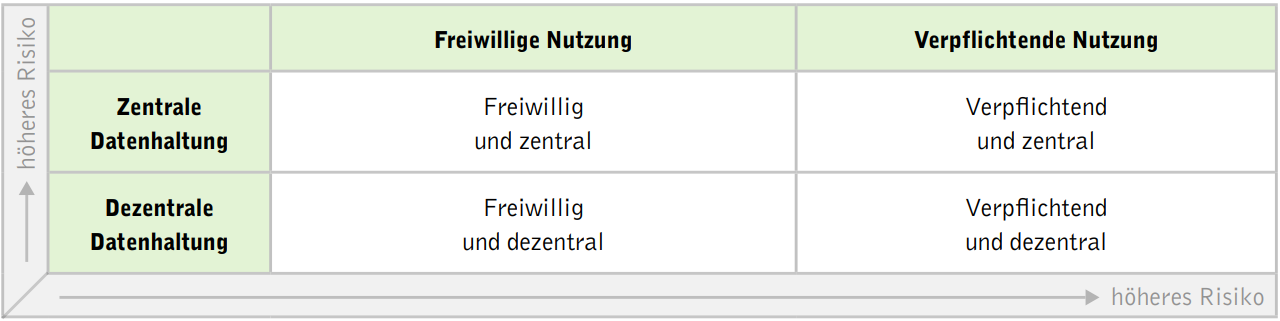
\includegraphics[width=0.7\textwidth]{DT-RisikoEinteilung.png}
    \caption{Risikobasierte Unterscheidung von Datentreuhandmodellen \cite{dt-blankertz2021neue}}
    \label{fig:dt-risikoeinteilug}
\end{figure}

\section{Anwendungsfälle}
\label{sec:dt-usecases}
Das mögliche Spektrum an Anwendungsfällen ist denkbar breit. In beinahe jedem Bereich, der eine große Menge an Daten benötigt oder verwaltet ist die Verwendung eines DTs ratsam \cite{dt-blankertz2021regulierung,dt-blankertz2021neue, dt-bundesdruckereiDatentreuhänder}. Beispiele dafür sind:
\begin{itemize}
    \item \textbf{Patientendaten.} Der DT sorgt für eine Pseudonymisierung von Patientendaten zur Bereitstellung an Forschungseinrichtungen. Hierbei behält der Patient die Kontrolle über seine Daten und kann selbst entscheiden, mit wem seine Daten geteilt werden.
    \item \textbf{Autonomes Fahren.} Beim autonomen Fahren werden große Datenmengen generiert, die seit 2017 per Gesetz gespeichert werden müssen \cite{dt-bundesdruckereiDatentreuhänder}. Leider ist die Zugehörigkeit der Daten rechtlich weder dem Autohersteller noch dem Autoinhaber zuzuschreiben \cite{dt-richter2020ddvtalk}. An dieser Stelle kann ein DT die Kommunikation erleichtern und exklusiven Zugang von beispielsweise Versicherungen oder Automobilkonzernen ausschließen.
    \item \textbf{E-Government.} Durch die Verwendung eines DTs können bei der behördlichen Verwaltung von Bürgerdaten große Fortschritte erzielt werden. Unter anderem müssen notwendige Informationen aus anderen Registern für Verwaltungsvorgänge nicht mehr vom Bürger bereitgestellt werden. Der Bürger erteilt lediglich seine Einwilligung zum Abruf der Daten zu Beginn des Verwaltungsvorgangs. Auf diese Weise können Verwaltungsvorgänge erheblich effizienter Ablaufen.
    \item \textbf{KI-Datenpools.} Eines der größten Probleme bei der Entwicklung von KI-Software ist der Zugang zu einer ausreichend großen Menge an Trainingsdaten. Ein DT kann solche Daten, die zur Verwendung für KI-Training freigegeben wurden, sammeln und pseudonymisiert an mehrere Interessierte verteilen. Dadurch entsteht ein einheitlicher Zugang zu Trainingsdaten, der gleichzeitig nur freigegebene Daten beinhaltet und so rechtlichem Streit über die Urheberschaft aus dem Weg geht.
    \item \textbf{Industrie.} In der Industrie besteht eine hohe Abhängigkeit von Warenbewegungen, sei es in Lieferketten, Logistik oder Handel. Durch die Verwendung eines DTs können Informationen über die Warenbewegungen pseudonymisiert an Warenempfänger weitergegeben werden. Vor allem in diesem Bereich besteht durch die Zusammenführung von Lieferinformationen in Kombination mit Algorithmen der Graphentheorie ein großes Innovationspotential.
    \item \textbf{PIMS.} Personal Information Management Systeme befassen sich grundsätzlich mit der Wahrung von personenbezogenen Daten und bieten ihren Nutzern mehr Kontrolle über ihre eigenen Daten. DT sind für solche Systeme vor allem von Vorteil, da sie dem Nutzer im Umgang mit personenbezogenen Daten wieder die Kontrolle über seine Daten zurückgeben.
\end{itemize}

\section{Bestehende Anreize}
Insgesamt bringt die Verwendung eines DTs keine direkten Nachteile mit sich. Wenn Daten ohnehin geteilt werden, behält der Nutzer bei der Speicherung der Daten über einen DT mehr Kontrolle über die Verwendung seiner geteilten Daten, als im Vergleich mit dem direkten Teilen mit Unternehmen. Durch den DT wird ihm ermöglicht, zu einem beliebigen Zeitpunkt das weitere Teilen seiner Informationen einzustellen. Vermutlich teilen deswegen Privatpersonen ihre Daten lieber mit DTs als auf direktem Weg. \cite{dt-tresor24study}

Allerdings gibt es nur wenige Vorteile, die die freiwillige Benutzung eines DTs reizvoll machen. Bei freiwilligen C2B DTs liegt die Entscheidung für oder gegen den Gebrauch des Treuhänders beim Nutzer. Es ist also an ihm abzuwägen, ob die Verwendung ausreichend Vorteile liefert. Im Fall von PIMS-Treuhändern wird die Verwendung von manchen Nutzern als erstrebenswert angesehen, da er mehr Kontrolle über die Verbreitung von persönlichen Daten erhält und selbst entscheiden kann, mit wem diese geteilt werden. Die Erkenntnisse von Jai et al. \cite{dt-jai2016privacy} zeigen hingegen, dass vor allem jüngere Erwachsene weniger Wert auf den Schutz ihrer persönlichen Daten legen.

Direkte Anreize zur Verwendung einer solchen Software sind bisher kaum vorhanden. An der Weitergabe der persönlichen Daten hat nur die Business-Seite einen konkreten Mehrwert \todo{proof}. Der Nutzer, der seine Daten freigibt, erhält keine Kompensation. Folglich kann es für einen freiwilligen DT mühsam sein, neue Nutzer zu gewinnen, um die Technologie als solche auszubauen.


%==================================================================================================


\chapter{Angreifermodelle und Anforderungen}
In diesem Kapitel werden zuerst die Angreifermodelle für das später entworfene Bezahl- und Reputationssytem definiert und anhand dieser die Anforderungen für die Systeme aufgestellt.
\label{chap:req}
\section{Definition der Angreifermodelle}
Angreifermodelle sind ein in der Informationssicherheit weit verbreitetes Konzept, mit dem sich die Stärke eines Systems gegen Angriffe eines theoretischen Angreifers zeigen lässt. Ein Angreifermodell besteht aus Angreiferzielen, Angreiferannahmen und Angreiferfähigkeiten. Angreiferzielen möchte ein Angreifer mit seinem Angriff erreichen. Angreiferannahmen legen die Ressourcen und das Umfeld des Angreifers fest. Angreiferfähigkeiten stellen dem Angreifer eine Liste an möglichen Angriffsmethoden zur verfügung. Zusammen ergibt sich aus diesen drei Komponenten ein Angreifer dessen Macht gerade so nicht ausreicht, damit der Angreifer sein definiertes Ziel erreicht. Eine ausführliche Erklärung von Angreifermodellen folgt in Kapitel \ref{chap:auswertung}. Hier werden fünf Angreifermodelle für die unterschiedlichen Akteure der später eingeführten Systeme aufgestellt.\\

Die Angreiferfähigkeiten beschränken sich bei allen folgenden Angreifermodellen auf die Verwendung von polynomialzeit Algorithmen und das Verfügen über unbegrenzten Speicherplatz.
\begin{enumerate}
    \item \textbf{Neugierig aber ehrlicher DT.} Das Ziel des neugierigen DTs ist, anhand der über ihn laufenden Kommunikation ausreichend Informationen über den DG und den DN zu erhalten, um die Handelsbeziehungen zwischen den beiden Akteuren verfolgen zu können. Er muss sich an die im Protokoll vorgeschriebenen Schritte halten und darf nur anhand der mitgeschnittenen Nachrichten Analysen tätigen.
    \item \textbf{Bösartiger DG.} Ein bösartiger DG möchte das System ausnutzen und ohne Daten zu teilen so viel Geld wie möglich erhalten. Er darf vom vorgegebenen Protokoll abweichen und kann über die erhaltenen Informationen frei verfügen, sowie diese öffentlich teilen.
    \item \textbf{Bösartiger DN.} Bösartige DN zielen darauf ab, die Identität der DG über mehrere Handel zu verlinken und so ein Pseudoym mit allen von diesem DG erhaltenen Daten zu erstellen. Zusätzlich möchte der DN für das Empfangen von Daten kein Geld ausgeben. Der bösaritge DN darf ebenfalls vom Protokoll abweichen und kann vorgeschriebene Berechnungswege ersetzen. Er kann Analysen anhand der mitgeschnittenen Nachrichten erstellen.
    \item \textbf{Neugierig aber ehrlicher Exchange.} In den Systemen die in den Abschnitten \ref{system:coingeneration} und \ref{system:payment} eingeführten werden, können Coins zum bezahlen des DG bei einem EX erstellt und eingelöst werden. Genauere Details werden in den jeweiligen Abschnitten genannt. Das Ziel des EX ist, die ausgestellten Coins beim späteren einlösen wieder zu erkennen und so Schlüsse über die Beziehung zwischen DN und DG zu ziehen. Außerdem möchte er einen Überblick darüber haben, welcher DN wie viele Coins erworben hat und wie viele davon bereits ausgegeben wurden. Der EX ist in den meisten Fällen an das Protokoll gebunden und kann nur an einer Stelle von diesem Abweichen. Er kann ebenfalls Analysen über die mitgeschnittenen Daten erstellen und probieren aus ihnen Informationen zu gewinnen.
    \item \textbf{Außenstehender Angreifer.} Ein außenstehender Angreifer ist nicht in die Kommunikation involviert, sondern möchte anhand sämtlicher übertragener Nachrichten zwischen zwei Akteuren herausfinden, wer mit wem kommuniziert und was in der Nachricht enthalten ist. Dafür kann er alle Nachrichten, die innerhalb der Protokolle ausgetauscht werden mitschneiden. Er kann auch mit den empfangenen Nachrichten selbst die Kommunikation mit einem Akteur aufnehmen und sich als ein Teilnehmer der Kommunikation ausgeben.
\end{enumerate}

\section{Anforderungen}
Aus den Angreifermodellen lassen sich einige Anforderungen an die Systeme ableiten. Da keiner der Angreifer sein Ziel erreichen darf, müssen die Anforderungen stark genug sein, um die Angreifer von ihrem Erfolg abzuhalten. Es wird zwischen funktionalen Anforderungen -- die genaue Funktionalitäten der Systeme beschreiben -- und nicht funktionalen Anforderungen -- die Eigenschaften der Funktionalitäten spezifieren -- unterschieden.
\subsection{Funktionale Anforderungen}
\label{enum:req:funktional}
\begin{enumerate}
    \item Ein Bezahlsystem ermöglicht es einem DG Geld für seine Daten zu erhalten.
    \item Ein Reputationswert gibt dem DN vor Erwerb der Daten eine Einschätzung über die durchschnittliche Datenqualität eines DG.
    \item Nach Erhalt von Daten muss ein DN den DG für die erhaltenen Daten bezahlen und diese Bezahlung auf Nachfrage nachweisen können.
    \item Nach Abschluss der Transaktion kann ein DN den entsprechenden DG aufgrund der Qualität der übermittelten Daten bewerten.
    \item Ein DG muss eine Bewertung seiner Daten ermöglichen.
    \item Ein DN kann pro Austausch nur genau eine Bewertung für einen DG abgeben. Mehrfache Bewertungen sind nur im Fall von mehrfachem Erwerb möglich.
\end{enumerate}

\subsection{Nicht funktionale Anforderungen}
\label{enum:req:nichtfunktional}
\begin{enumerate}
    \item \textbf{Anonymität.} Die Identität des DG darf durch den Austausch von Zahlungsmitteln oder durch dessen Reputation nicht offengelegt werden.
    \item \textbf{Unverkettbarkeit.} Mehrere Transkationen eines DG dürfen keine Informationen über den Zusammenhang der Transaktionen aufweisen. 
    \item \textbf{Zeitsensitivität.} Der Bezahlvorgang muss in vernachlässigbarer Zeit geschehen.
    \item \textbf{Skalierbarkeit.} Die Rechenzeit des Systems soll bei linear steigender Menge an Transkationen auch mit linearem Zeitaufwand zunehmen.
    \item \textbf{Vertraulichkeit.} Die kommunizierten Daten dürfen nicht durch unbefugte Dritte ausgelesen werden können.
    \item \textbf{Integrität.} Die kommunizierten Daten dürfen nicht unbemerkt durch unbefugte Dritte verändert werden.
\end{enumerate}

\chapter{Verwandte Arbeiten}
In diesem Kapitel werden bestehende Arbeiten vorgestellt, die eine dichte Verbindung zu dem Thema dieser Bachelorarbeit haben. Dafür wird das Produkt der verwandten Arbeit erklärt und anschließend erläutert, warum diese in dem Umfeld eines DTs nicht eingesetzt werden kann. Die verwandten Arbeiten beziehen sich zuerst auf weitere Bezahlsysteme und behandeln danach einige Reputationssystem sowie Bausteine, die für die Konstruktion des hier dargelegten Bezahl- und Bewertungssystems essentiell sind.

\section{GNU Taler}
\label{subsec:gnu}
Das im Paper ``Enabling Secure Web Payments with GNU Taler`` von J. Burdges et al. eingeführte Zahlungssystem GNU Taler ist ein elektronisches Online-Zahlungssystem, das Datenschutz für Customer und Mechanismen zur steuerlichen Nachverfolgung für Merchants bietet \cite{gnu-burdges2016enabling}. Es verwendet einen EX, um Münzen mithilfe von blinden Signaturen zu Erstellen und zwischen Nutzern und Händlern zu transferieren. Im Folgenden werden diese Münzen als Taler bezeichnet. Das System basiert auf vier übergeordneten Rollen, deren Interaktion grob in Abbildung \ref{fig:gnu_taler_overview} skizziert sind. Der Customer möchte ein Gut oder eine Dienstleistung bei dem Merchant erwerben und bezahlt diesen dafür mit Talern, die er beim EX erworben hat. Der Merchant kann die erhaltenen Taler wieder beim EX für herkömmliche Währungen eintauschen. Ein Auditor überprüft währenddessen die Liquidität des EX, um sicherzustellen, dass dieser auch bei Datenverlust von Talern noch in der Lage ist, allen Beteiligten Auszahlungen zu ermöglichen.

\begin{figure}[H]
    \centering
    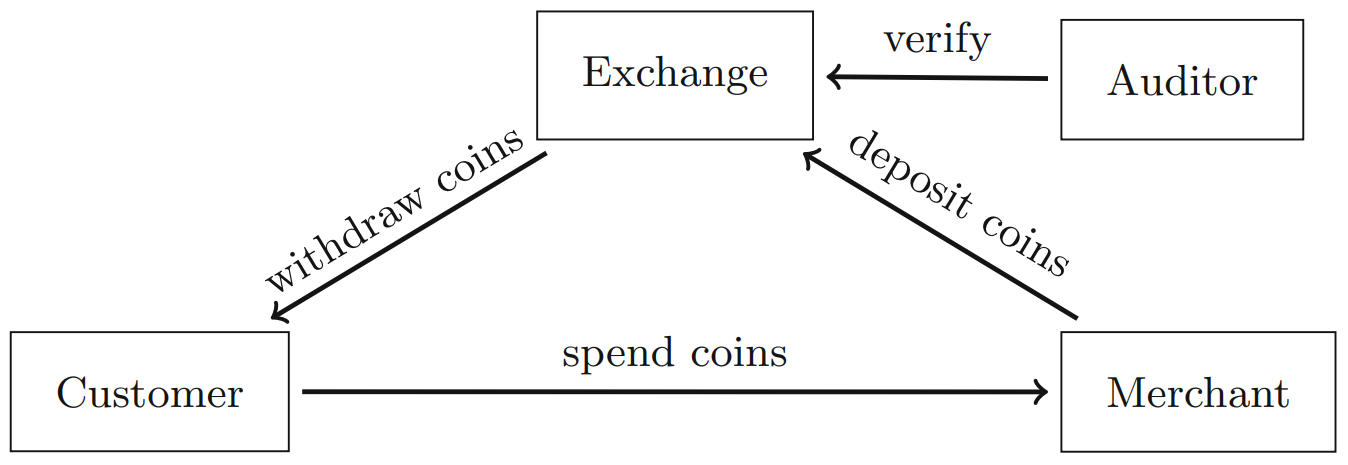
\includegraphics[width=0.7\textwidth]{gnu_system_graphic.png}
    \caption{Grundlegender Ablauf des GNU Taler Systems \cite{gnu-burdges2016enabling}}
    \label{fig:gnu_taler_overview}
\end{figure}

\textbf{Taler abheben.} Damit ein Customer Geld auf sein Wallet laden kann, muss er sich zuerst bei seiner Bank anmelden. Sollte die Bank GNU Taler nativ unterstützen, so kann der Customer in einem Formular eine Summe auswählen, die er in Taler übertragen möchte und einen EX, über welchen der Tausch abgewickelt wird. Nachdem der Customer die Transaktion bestätigt hat, wird die ausgewählte Summe transferiert, der EX signiert die äquivalente Summe an Talern und überträgt diese in das Wallet des Customers.\\

\textbf{Taler ausgeben.} Gehen wir von der Situation aus, dass ein Customer bei einem Merchant (hier ein Onlineshop) etwas erwerben möchte. Nach der Auswahl des Produktes und GNU Taler als Zahlungsmittel erstellt der Merchant einen Zahlungsvertrag, der Details wie den Gesamtpreis, mögliche offene Umwandlungsgebühren und akzeptierte EXs beinhaltet und sendet diesen an das Wallet des Customers. Wenn der Customer daraufhin die Zahlung übermittelt, so leitet der Merchant die erhaltenen Taler direkt an den EX weiter. Wenn der EX den Eingang bestätigt, kann der Merchant dem Customer die Transaktion bestätigen und der Kauf ist abgeschlossen.

In dem DT-Modell eignet sich GNU Taler nur teilweise als Zahlungssystem. Der DG stellt den Merchant dar, der seine Daten als digitales Gut anbietet. Der DN ist hier in der Rolle des Customers und möchte diese Daten erwerben. Sollte der DG der Anfrage des DN zustimmen, so würde er einen Zahlungsvertrag formulieren, um den Anspruch auf seine Vergütung zu formalisieren. Allerdings soll der DG im DT-Modell so gut wie möglich vor Informationsgewinnung geschützt werden. Bei dem von GNU Taler vorgeschlagenen Prozess besteht eine direkte Kommunikation zwischen DG und DN, was viele schützenswerte Informationen über die Identität des DG (beispielsweise seine IP-Adresse) preisgibt.

\section{Bitcoin}
\label{sec:bitcoin}
Die Idee hinter Bitcoin entstand 2008 durch eine Person oder Gruppe mit dem Namen Satoshi Nakamoto. Heute ist Bitcoin die mit Abstand weit verbreiteteste Onlinewährung weltweit \cite{btc-beginnerGuide}. Sie basiert auf einem verteilten öffentlichen Register, das alle Transaktionen pseudonymisiert für jeden einsehbar macht und speichert. Dieses Register ist auch als Blockchain bekannt.

\begin{figure}[h]
    \centering
    \caption{Blockchain mit Transaktionen \cite{btc-nakamoto2008bitcoin}}
    \label{fig:btc_blockchain}
    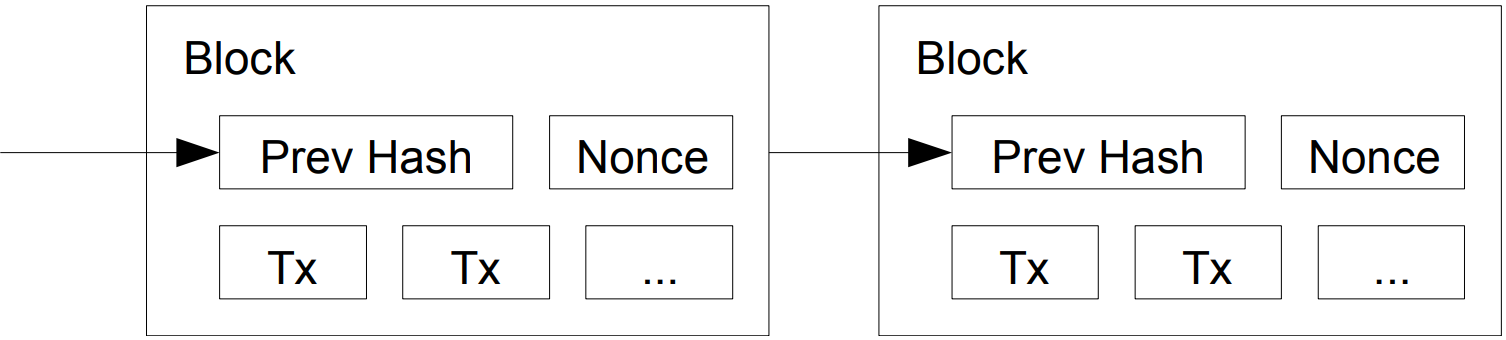
\includegraphics[width=0.5\linewidth]{BitcoinBlockchain.png}
\end{figure}

Die Blockchain ist eine Kette an Blöcken, die jeweils den Hashwert des vorherigen Blocks und neue Transaktionen speichert. Durch den Hashwert des vorherigen Blocks entsteht eine Abhängigkeit, durch die jeder Block auf seinem Vorgänger basiert, wie in Abbildung \ref{fig:btc_blockchain} zu sehen ist. Ein neuer Block entsteht durch einen sogenannten Proof of Work. Dieser ist das Wissen über eine Zufallszahl, deren Hash mit $x$ 0 bits beginnt, welche ausschließlich durch das wiederholte Ausprobieren von Zufallszahlen gefunden werden kann. Dieser Vorgang wird als Bitcoin Mining bezeichnet. Sobald eine solche Zahl gefunden wird, kann der aktuelle Block abgeschlossen werden und alle folgenden Transaktionen werden in dem nächsten Block gespeichert \cite{btc-nakamoto2008bitcoin}.

Der Algorithmus, der bestimmt wie schwer das Erbringen des Proof of Works ist, kann jederzeit dynamisch an die Rechenleistung der Miner angepasst werden, so dass im Schnitt alle 10 Minuten ein neuer Block gefunden wird \cite{btc-Zaghloul2019Bitcoin}. Um also eine vergangene Transaktion auf der Blockchain zu verändern, müsste ein Angreifer für jeden darauffolgenden Block selbst einen Proof of Work berechnen. Ein Angreifer kann deswegen nur eine vergangene Transaktion ändern, wenn er allein mehr Rechenleistung besitzt als alle anderen Miner zusammen.

In dem Moment, in dem ein Block abgeschlossen und der nächste begonnen wird, sind alle Transaktionen auf dem abgeschlossenen Block ein Mal bestätigt. Das bedeutet, dass keine der Transaktionen einen Coin zum zweiten Mal ausgibt. Dies ist eine essentielle Sicherheitsmaßnahme von Blockchain Kryptowährungen da Blockchain dezentralisiert und ohne neutralen Überprüfer funktioniert. Es ist also an allen Beteiligten, die pseudonymisierten Transaktionen des Blocks auf doppelte Ausgaben zu überprüfen. Ein Angreifer kann versuchen den gleichen Bitcoin in zwei Transkationen zu verwenden, von denen die erste den Bitcoin zurück auf das Wallet des Angreifers sendet und die zweite einen Dienstleister bezahlt. Sollte beim Erstellen des nächsten Blockes die erste Transkation gewählt werden, so wird die zweite -- die den Dienstleister bezahlt -- ungültig. Um solche Angriffe zu verhindern, können Verkäufer auf Bestätigung der Transkationen durch das Erstellen eines neuen Blocks warten. Im Fall von Bitcoin wird empfohlen, 6 weitere Blöcke abzuwarten bis eine Transaktion wirklich abgeschlossen ist \cite{btc-Zaghloul2019Bitcoin}. In Kombination mit einer durchschnittlichen Berechnungsdauer von 10 Minuten dauert es also ca. eine Stunde, bis eine Transaktion auf der Blockchain als Sicher angesehen wird.
Durch den enormen Rechenaufwand, der benötigt wird um einen Block abzuschließen, kann grob überschlagen werden, wie viel Energie in eine einzelne Bitcointransaktion fließt. In \cite{btc-energyConsumption} wird eine Transaktion auf 703,25 kWh geschätzt, was ca 470.000 VISA Transaktionen entspricht.

Allein die lange Bestätigungsdauer einer Transaktion schließt Bitcoin bereits für die Verwendung in diesem System aus. Da eine Stunde nicht mehr als vernachlässigbare Zeit angesehen werden kann, ist die Anforderung an Zeitsensitivtät nicht erfüllt. Hinzu kommt der gigantische Stromverbrauch, welcher die Skalierbarkeit von Bitcoin -- unabhängig von der definierten Anforderung -- in Frage stellt. 

\section{Ethereum}
\label{sec:ethereum}
Ethereum ist die Blockchainanwendung hinter der am zweithäufigsten verbreiteten Kryptowährung Ether \cite{eth-marketCapitalisation}. Es wurde 2013 von Vitalik Buterin erfunden und ist eine Plattform, die es Entwicklern ermöglicht Anwendungen auf der Blockchain zu entwickeln. Es liefert eine Turing-vollständige Programmiersprache die es Entwicklern erlaub, eigene Währungen in unter 20 Zeilen Code zu schreiben \cite{eth-buterin2013ethereum}. Sämtliche dort entwickelte Währungen oder sogenannte Smart Contracts werden über die Ethereum Blockchain pseudonymisiert veröffentlicht. 

Durch die Verwendung der Blockchain decken sich einige Eigenschaften mit Bitcoin. Ethereum besteht genauso aus einer Reihe an Blöcken, die kontinuierlich ihren Vorgänger referenzieren. Bis 2022 nutzte Ethereum ebenfalls einen Proof of Work Ansatz. Doch seit 2022 basiert Ethereum auf einem sogenannten Proof of Stake Konzept \cite{eth-explainerInvestopia}. Das bedeutet, dass es eine Gruppe an Validierern gibt, welche die Transaktionen innerhalb der Blöcke überprüfen. Um ein Validierer zu werden, muss ein Starteinsatz von 32 Ether gezahlt werden. Alternativ kann sich ein Nutzer einem Validiererpool anschließen und einen kleineren Starteinsatz zahlen.

Die Aufgabe eines Validierers ist es, unzulässige Transaktionen festzustellen. Im Falle eines Angriffs auf einen Block wird der Block von Gasper (Einer Mischung des Casper-FFG Protokolls und LMD Ghost Algorithmus \cite{eth-buterin2020combining}.) markiert. Anschließend entscheiden die Validierer, ob der Block zugelassen oder blockiert werden soll. Bösartige Validierer werden dadurch bestraft, dass ihr Starteinsatz nach und nach ``verbrannt`` wird. Verbrannt bedeutet hier, dass der Einsatz an ein Wallet ohne SK gesendet wird, was die Coins unwiderruflich verschlüsselt. Durch diesen alternativen Ansatz kann der große Rechenaufwand von Bitcoin umgangen werden.\\

Die Verwendung einer Blockchain stellt hier wieder das Problem der Zeitsensitivität dar. Zwar dauert das Erstellen eines Blocks bei Ethereum nur 12 Sekunden \cite{eth-timePerBlock}, dafür wird allerdings eine Mindestanzahl von 30 Blöcken empfohlen, bevor eine Transaktion für gültig erklärt wird \todo{proof}. Somit entsteht eine Wartezeit von circa sechs Minuten, was bei weitem besser ist als bei Bitcoin. Trotzdem sind sechs Minuten keine vernachlässigbare Zeit, weshalb auch Ethereum nicht für dieses System verwendet werden kann.


\section{Privacy Pass}
\label{sec:privacy-pass}
Privacy Pass ist eine Browsererweiterung, die den Komfort der Internetbenutzung für Nutzer eines VPNs erhöht. Durch einen VPN kommuniziert ein Nutzer nach außen mit der gleichen IP-Adresse, wie viele weitere Nutzer. Dies steigert die Anonymität gegenüber Webseitenbetreibern \cite{pp-Abbas2023Security}, allerdings kann die geteilte IP-Adresse durch bösartiges Verhalten anderer Nutzer von Content Delivery Networks (CDN) einen schlechten Ruf erhalten. Ein CDN ist ein Service der häufig angefragte Webseiten wie google.de in seinem Cache aufbewahrt und so die Zugriffszeit -- die durch physikalische Distanzen zwischen Nutzer und Server entsteht -- verkürzt \cite{pp-cdn}. Die Folgen eines schlechten Rufs der IP-Adresse sind, dass alle Nutzer der IP-Adresse für Anfragen zuerst ein CAPTCHA lösen müssen, das prüft, ob ein Mensch oder ein Bot die Anfrage gestellt hat. Dies ist eines der Sicherheitsfeatures das ein CDN anbietet \cite{pp-Ghaznavi2021Content}. Privacy Pass zielt darauf ab, eine tokenbasierte Alternative anzubieten, bei der vorab ein CAPTCHA gelöst wird und dafür eine Menge an Token ausgestellt wird. Das nächste Mal wenn ein CDN ein CAPTCHA präsentiert kann der Nutzer einen Token einlösen und dieses so überspringen \cite{pp-davidson2018privacy}.

\subsection{Funktionsweise}
Das System ist in eine sogenannte Signierphase und eine Einlösephase aufgeteilt. Die Signierphase startet, nachdem der Nutzer erfolgreich ein CAPTCHA gelöst hat. Sie ist dafür zuständig, dem Nutzer eine Anzahl an Token auszustellen, die durch den Server signiert sind. Die Einlösephase beginnt, wenn ein CDN ein CAPTCHA für den Zugang zu einem Webinhalt fordert. Bei ihr wird einer der gespeicherten, signierten Token eingetauscht, um die Lösung des CAPTCHAs zu überspringen. 

\begin{figure}[h]
    \centering
    \begin{subfigure}[b]{0.45\textwidth}
        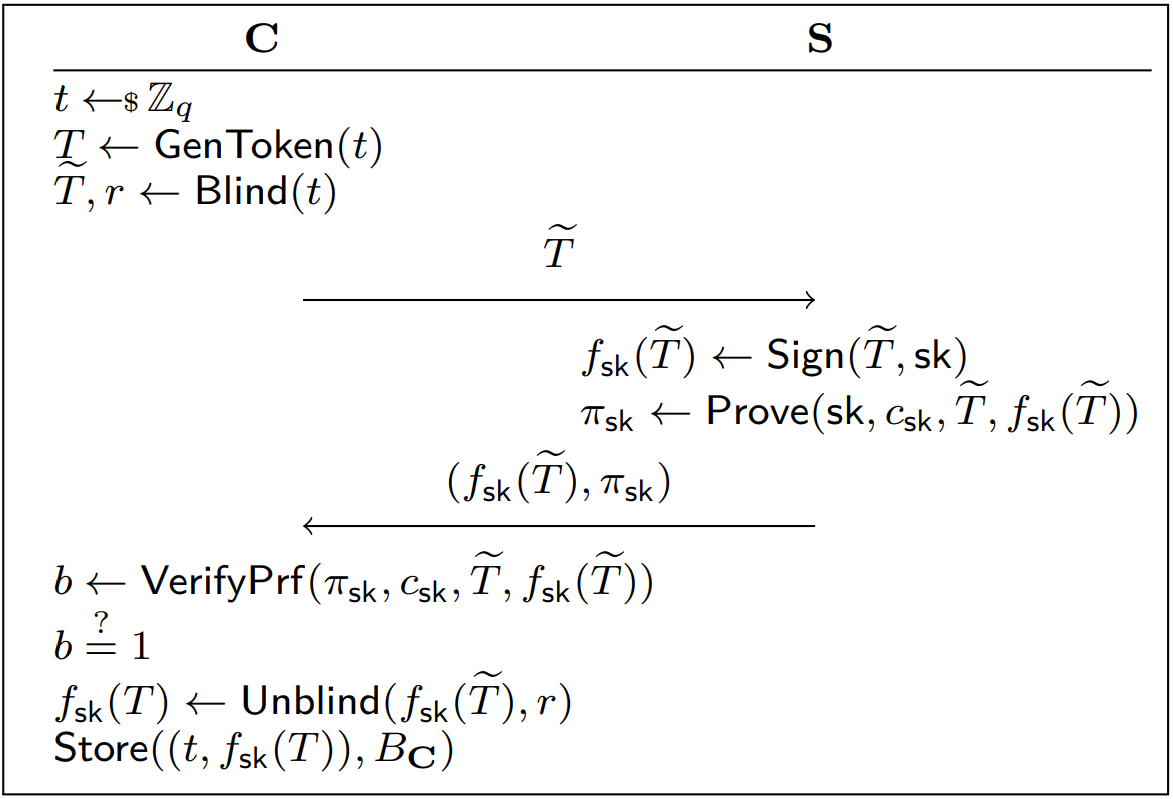
\includegraphics[width=\textwidth]{pp_signphase.png}
        \caption{Signierphase von Privacy Pass \cite{pp-davidson2018privacy}}
        \label{fig:pp-signingphase}
    \end{subfigure}
    \hfill
    \begin{subfigure}[b]{0.45\textwidth}
        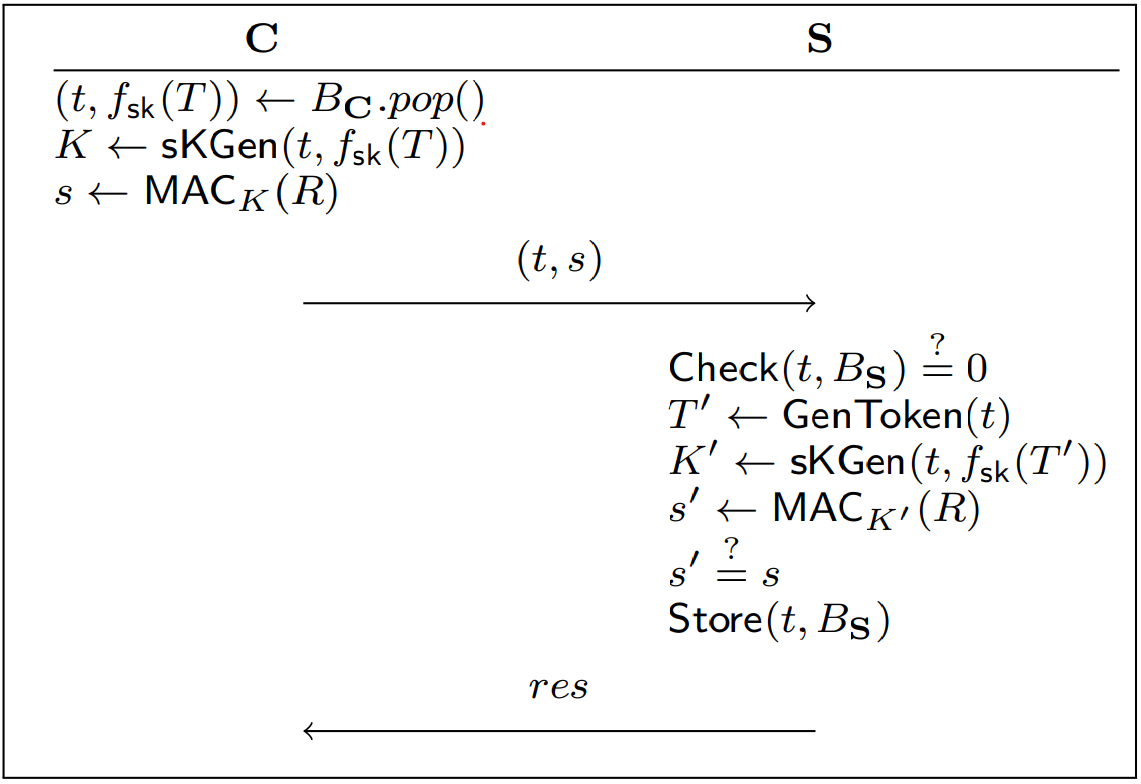
\includegraphics[width=\textwidth]{pp-redemptionphase.png} 
        \caption{Einlösephase von Privacy Pass \cite{pp-davidson2018privacy}}
        \label{fig:pp-redemptoinphase}    
    \end{subfigure}
\end{figure}
\paragraph{Signierphase.}
Die Abbildung \ref{fig:pp-signingphase} zeigt die Berechnung beim Durchlaufen einer Signierphase. Zuerst erstellt der Nutzer einen zufälligen Token $T$. Dieser Token wird geblendet und an den Server gesendet. Die Funktionalität des Blendens wird in Abschnitt \ref{sec:partBlindSig} genauer beschrieben. Beim Server angekommen beginnt dieser damit, den Token mit seinem $sk$ zu signieren. Anschließend erstellt er einen sogenannten Batch Discrete Log Equivalence Proof (BDLEQ), um zu beweisen, dass er für jeden Nutzer einen gleichen $sk$ verwendet. Der signierte Token und der BDLEQ werden wieder an den Nutzer gesendet. Dieser prüft die Korrektheit des BDLEQ Beweises, entblendet den signierten Token und speichert ihn für eine spätere Verwendung. 

\paragraph{Einlösephase.}
Abbildung \ref{fig:pp-redemptoinphase} zeigt den Ablauf der Einlösephase, in der der Nutzer damit beginnt, einen gespeicherten, signierten Token aus seinem Speicher auszulesen. Anschließend verwendet er einen anfragenabhängigen Wert wie beispielsweise die Domain der angefragten Seite und bildet einen MAC um mit dem signierten Token als Schlüssel. Dadurch wird sichergestellt, dass ein Token mit einer Anfrage verknüpft ist und die Integrität geschützt wird. Daraufhin sendet er das Tupel aus Tokengrundform $t$ und Anfragenparameter $s$ an den Server. Der Server kann nun prüfen, ob $t$ bereits für eine vorherige Anfrage verwendet wurde und kann anschließend alle Schritte des Nutzers berechnen. Erhält er dabei $s'=s$, dann ist der Token valide, das CAPTCHA kann übersprungen werden und der Nutzer erhält Zugriff auf die angefragte Webressource.

\paragraph{Batch Discrete Log Equivalence Proof.}
Beim dem BDLEQ handelt es sich um einen Zero Knowledge Proof (ZKP). ZKPs sind ein in der Kryptographie auftretendes Beweismuster, dass das Wissen über einen Wert belegen kann, ohne den Wert tatsächlich zu nennen. Der hier verwendete Discrete Log Equivalence Proof kann dazu verwendet werden, die Gleichheit von zwei diskreten Logarithmen zu zeigen. Für die genaue Anwendung wird hier auf die Arbeit von Davidson et al. \cite{pp-davidson2018privacy} verwiesen. Dieser Beweis wird aus dem Grund erstellt, dass ein CDN ansonsten für das Signieren von jedem Token ein unterschiedliches Schlüsselpaar verwenden kann. Die Folgen davon sind eine mögliche Deanonymisierung, da der CDN beim Einlösen des Tokens anhand des verwendeten Signierschlüssels -- der einmalig ist -- den Signierzeitpunkt und zugehörigen Nutzer bestimmen kann. Der DLEQ liefert dem Nutzer die Sicherheit, dass der diskrete Logarithmus des zum signieren verwendeten SK der gleiche ist, wie ein von CDN öffentlich bekannt gegebener diskreter Logarithmus. Davidson et al. beschreiben zudem einen Weg den DLEQ in einer Sammelform zu formulieren, sodass ein Beweis für eine Liste an Token gilt \cite{pp-davidson2018privacy}, was Rechenaufwand spart.

Im Grunde lässt sich Privacy Pass gut im DT-Modell anwenden. Unter der Annahme, dass ein DN hier ein Nutzer ist, kann er Token bei dem DT erwerben, speichern und zu einem späteren Zeitpunkt wieder ausgeben. Da die Token blind signiert werden, wird vermieden, dass der DT die in den unterschiedlichen Phasen verwendeten Token zueinander verlinken kann und Zusammenhänge zwischen Einlösen und Ausgeben herstellen kann. Der DT kann eine weitere überprüfende Instanz verwenden, wie in \cite{pp-davidson2018privacy} beschrieben wird, um den Aufwand der Überprüfung auszulagern. Einige Punkte sprechen jedoch gegen die direkte Verwendung von Privacy Pass. 
\begin{enumerate}
    \item Die Token haben keinen Wert. Bei Bezahlungsmitteln ist es essenziell einen bestimmten Preis bezahlen zu können. Dafür wären entweder mehrere unterschiedliche Tokens von Nöten, oder Token, die einen monetären Wert gespeichert haben. Bei der Speicherung eines monetären Wertes gibt sich das Problem der Beweisbarkeit. Wenn ein Token geblendet und für den DT nicht lesbar ist, stellt sich die Frage, wie sichergestellt werden  kann, dass der richtige Wert eingehalten wurde und der DN sich nicht mehr Geld aufschreibt als ihm zusteht. Andernfalls kann nur ein Vielfaches von einem Token gezahlt werden was dazu führt, dass es keine präzise Preisvergabe gibt, oder bei jeder Transaktion eine große Menge an Token validiert werden muss.
    \item Ein Nutzer interagiert sowohl zum Einlösen als auch zum Ausgeben nur mit dem Server und nicht mit einem Verkäufer, dem er seine Token im Tausch anbietet. Es existiert hier also kein dritter Akteur wie bei GNU Taler, der erhaltene Token einlöst.
    \item Die Token können ähnlich wie bei GNU Taler nicht direkt an den Verkäufer weitergegeben werden, da dadurch eine direkte Verbindung zwischen DN und DG entsteht, welche schützenswerte Informationen offen legt.
\end{enumerate}

\section{Privacy-Preserving Reputation Management}
\label{subsec:rep}
In ihrem Paper beschreiben R Petrlic et al. ein Reputationssystem um Nutzern den Dienst eines Dienstleisters anonym bewerten zu lassen und so anderen Nutzern eine Einschätzung über die Qualität der Dienstleistung zu geben \cite{petrlic2014privacy}. Es werden drei Rollen charakterisiert. Ein Reputation Provider $RP$, der sich um das Verwalten der verschiedenen Reputationswerte kümmert. Eine Menge an Service Providern $SP$, die einen Dienst anbieten der durch Nutzer bewertet werden soll. Und zuletzt eine Menge an Nutzern $U$, die die Dienstleistung der Service Provider bewerten. Dabei kann keiner der Nutzer gleichzeitig ein Service Provider $SP$ sein und es gilt $U \cap SP = \varnothing$. 

Der im Paper beschriebene Ablauf des Bewertens eines $sp \in SP$ durch einen Nutzer $u \in U$, umfasst grob die Erstellung eines Schemas für einen Bewertungsvektors durch $sp$, welcher von $u$ später verwendet wird, um den $sp$ zu bewerten. Nach dem $sp$ diesen Vektor mit dem $RP$ kommuniziert hat, kann $u$ eine Dienstleistung von $sp$ in Anspruch nehmen. Dieser antwortet, zusätzlich zur Erbringung der Dienstleistung, mit einer Beschreibung des Bewertungsvektors, einem Schlüsselpaar und einem Token. Dank der Beschreibung kann der Nutzer selbst einen Bewertungsvektor erstellen, in welchen er seine Bewertung der Dienstleistung einbaut. Im Anschluss wird dieser mit dem Schlüsselpaar verschlüsselt, signiert und zusammen mit dem signierten Token an den $RP$ gesendet. Der Token dient hier zur Erkennung von doppelten Bewertungen. 

Die Berechnung der Reputation ist in Zeitslots eingeteilt, damit ein $sp$ nicht in der Lage ist einen alten Reputationswert anzugeben. Wenn nun ein Nutzer $u$ den Reputationswert eines $sp$'s einsehen möchte und der Wert für den gewünschten Zeitraum noch nicht bestimmt wurde, so muss dieser zwischen $RP$ und $sp$ berechnet werden. Hierfür bestimmt $RP$ die Summe aller verschlüsselten Bewertungsvektoren für den Zeitraum und sendet diese zusammen mit weiteren Prüfwerten an $sp$. Dieser kann die übermittelten Werte prüfen und auf eine Blacklist hinzufügen, um Replay Attacken von $RP$ auszuschließen. Wenn die Überprüfung gelingt, signiert $sp$ die Summe der Vektoren zusammen mit einer ID und verifiziert somit den neuen Reputationswert an $RP$. 

Bei einer Anfrage des Reputationswertes von $sp$ durch $u$ schickt der $sp$ eine Reihe an Werten zu $u$. Diese erlauben es $u$, den Bewertungsvektor zu interpretieren und zu prüfen, ob der übermittelte Werte sowohl aktuell ist, als auch nicht beeinflusst wurde. 
Das Konzept von Petrlic et al. bietet unter anderem Schutz vor: 
\begin{enumerate}
    \item \textbf{Whitewashing}, bei dem sich ein $sp$ mit schlechter Reputation als neuer $sp$ ausgeben kann, um somit den Wert zurückzusetzen.
    \item \textbf{Transaction-independent Ratings}, bei denen ein Nutzer die Dienstleistung bewerten kann, obwohl er besagte Dienstleistung nicht in Anspruch genommen hat.
    \item \textbf{Sybil Attacks.} Ein Nutzer bewertet eine Dienstleistung unter mehreren Identitäten und täuscht so seine Meinung als Gruppenmeinung vor.
    \item \textbf{Delta Analysis.} Eine teilweise Deanonymisierung des Nutzers durch Vergleichen von gesammelten Bewertungen in unterschiedlichen Zeitabständen.
\end{enumerate} 
Für die Verwendung im DT-Modell ist dieses Reputationssystem nicht geeignet. Zum einen ist das Konzept darauf ausgelegt, dass zu Beginn eine Kommunikation zwischen dem $sp$ und $u$ besteht, so dass der Reputationswert direkt durch den $u$ abgefragt werden kann. Dadurch würde in den angewendeten Rollen eine direkte Verbindung zwischen DG und DN bestehen, was hier vermiden werden soll. Zum anderen ist der zur Bewertung übertragene Schlüssel ein homomorpher Schlüssel, sodass der $RP$ alle gesammelten Bewertungen aufaddieren kann, ohne diese vorher zu entschlüsseln. Das zwingt den $sp$ für jede Bewertung den gleichen Schlüssel anzugeben, da sonst die Berechnung fehlerhaft wird. Durch das Angeben des selben Schlüssels könnte ein DN den DG -- den er bewertet -- wiedererkennen und unter einem Pseudoym alle Handel mit ihm verlinken.

In der Literatur sind weitere Beispiele für (anonyme) Reputationssysteme zu finden. In \cite{rep-muller2008sybil} wird ein System vorgestellt, das anonymes bewerten mithilfe einer Anonymitätsschicht ermöglicht. Diese Schicht stellt sicher, dass weder der Bewertende noch der Bewertete weiß, wer der andere ist. Allerdings kennt diese Anonymitätsschicht die IDs beider Teilnehmer, was im DT Kontext bedeuten würde, dass der DT die Handlungsbeziehung zwischen DG und DN nachvollziehen kann. Zusätzlich erlaubt das System mehrfaches Bewerten was gegen die gesetzen Anforderungen verstößt.

Das in \cite{rep-androulaki2008reputation} vorgestellte System bietet eine Reputationsvergabe über das von Chaum entworfene ecash System. Es ist ebenfalls für Peer to Peer Netzwerke entworfen und erlaubt es Nutzern ein Pseudoym zu erstellen mit welchem sie ecash Coins versenden und empfangen können. Die Coins können bei einer zentralen Bank eingetauscht werden, die zusätzlich die Reputation der Pseudonyme verwaltet. In dem Paper wird jedoch erwähnt, dass das System weder in Echtzeit noch mit hoher Performanz läuft. Aufgrund einer fehlenden Implementation liegen keine Zahlen für einen direkten Vergleich vor. Allerdings kann dadurch angenommen werden, dass das System nicht die Anforderung an die Zeitsensitivität erfüllt. Zusätzlich werden Pseudonyme innerhalb des Systems durch RSA PKs dargestellt. Damit ein DG beim handeln seine Anonymität bewahrt, muss er für jeden Handel ein neues Pseudonym -- also ein neues RSA Schlüsselpaar -- erstellen. Diese Operation alleine genügt, damit die Zeitsensitivität verletzt wird.

\section{Partiell blinde Signaturen}
\label{sec:partBlindSig}

Partiell blinde Signaturen ähneln sich vom Effekt stark zu blinden Signaturen von Chaum aus \cite{chaum1983blind}. Bei blinden Signaturen kann ein Nutzer eine Nachricht $x$ mit einer Funktion $c(\cdot)$ blenden. Das Ergebnis davon ist $c(x)$. Die Funktion $c(\cdot)$ besitzt ein Inverses $c'(\cdot)$, sodass $c'(c(x)) = x$. Das Ergebnis $c(x)$ kann an eine signierende Instanz übertragen werden. Wenn diese ihre Signatur $s(\cdot)$ hinzufügt, entsteht $s(c(x))$. Sobald der Nutzer die signierte, geblendete Nachricht zurück erhält, kann er sie entblenden und erhält $c'(s(c(x))) = s(x)$. Auf diesem Weg kann der Nutzer eine Nachricht signieren lassen, ohne dass die signierende Instanz Kenntnisse über die Nachricht erhält. Der bei partiell blinden Signaturen entscheidende Unterschied ist, dass es einen Infowert gibt, der sowohl dem Nutzer, als auch dem Signierenden bekannt ist. Der Infowert kann genutzt werden, damit der Signierende möglicherweise Prüfungen durchführen und entscheiden kann, ob er die Nachricht wirklich signieren möchte. Diese Eigenschaft wird im späteren Verlauf beispielsweise dazu verwendet, einen Coin partiell blind zu signieren. Hierbei ist es essenziell, dass der Signierende den monetären Wert des Coins prüfen kann, da ein Nutzer sonst freie Kontrolle über den Wert seines eigenen Coins hat. Mit partiell blinden Signaturen kann genau dies gewährleistet werden. Dabei ist der monetäre Wert des Coins die Info und der kryptographische Wert des Coins die Nachricht. Nun kann der Signierende prüfen, ob der monetäre Wert wie vereinbart ist und kann den kryptographischen Wert des Coins blind signieren. Der entscheidende Aspekt ist der Zusammenhang zwischen Info und Nachricht, da sonst der monetäre Wert des Coins nach dem Signieren durch den Nutzer verändert werden könnte. Um dies zu verhindern, verwendet das Verfahren den Hashwert der Info als Teil der Signatur, so dass diese nur gültig ist, solange die Info unverändert bleibt.

\subsection{Funktionsweise}
\begin{figure}[h]
    \centering
    \includegraphics*[width=0.6\textwidth]{partBlindSig.png}
    \caption{Ablauf einer partiell blinden Signatur \cite{abe2000provably}}
    \label{fig:partBlindSig}
\end{figure}
Die Durchführung einer partiell blinden Signatur besteht aus vier Schritten. Diese vier Schritte sind notwendig, um die Abhängigkeit von der Nachricht $msg$ und der Info herzustellen. Der gesamte Ablauf ist in Abbildung \ref{fig:partBlindSig} dargestellt. Es wird davon ausgegangen, dass vor dem ersten Schritt beide Parteien über den Infowert verfügen. Der Signierende bildet zuerst den Hashwert der Info, signiert diesen und schickt ihn an den Nutzer. Dieser bildet den gleichen Hashwert der Info und verwendet die erhaltenen Werte zusammen mit einer Reihe an Zufallszahlen, um $\alpha$ und $\beta$ zu berechnen. $\epsilon$ ist der darauffolgende Hashwert von $\alpha,\beta,z$ und $msg$. Hier fließt die bereits signierte Info über $\alpha$ und $\beta$ mit ein. Kurz darauf empfängt der Signierende $e$, welches nun sowohl Info als auch msg beinhaltet. Dieses $e$ kann er nun verwenden, um Info und $msg$ zu signieren und die aus den Berechnungen resultierenden Werte an den Nutzer zu senden. Der Nutzer kann dadurch $\rho,\omega,\sigma,\delta$ bestimmen und speichern. Möchte der Nutzer zu einem beliebigen Zeitpunkt die Signatur auf ihre Gültigkeit prüfen, so kann er $\omega + \delta$ mit  $H (g^\rho y^\omega || g^\sigma z^\delta || z || msg)$ vergleichen. Wenn die Werte übereinstimmen, ist die Signatur valide.

Durch die Verwendung der Info als Teil der Signatur ist gewährleistet, dass die Signatur nur bei einer unveränderten Info und $msg$ valide bleibt. Denn sollte sich die Info oder $msg$ ändern, dann würde die Rechnung zur Überprüfung einen anderen Hash erzeugen, welcher nicht mehr mit $\omega+\delta$ übereinstimmt. Insgesamt ist das partiell blinde Signaturen Schema etwas umständlicher als Chaums blinde Signaturen. Dennoch bietet es die Möglichkeit, einen öffentlichen Wert zu kommunizieren und dessen nachträgliche Änderung zu verhindern.


\section{Elliptische Kurven Kryptographie}
\label{sec:ecc}
Die Kryptographie über elliptische Kurven (ECC - elliptic curve cryptography) ist ein Zweig der Kryptographie, der bereits seit 1985 besteht \cite{ecc-miller1985use}. Hierbei geht es um das Ver- und Entschlüsseln von Nachrichten anhand von Punkten auf einem elliptischen Graph, was verglichen mit RSA, das auf der Faktorisierung großer Primzahlen basiert, erhebliche Performanzsteigerung liefert.

\subsection{Trapdoor functions}
Das asymmetrische RSA Verschlüsselungsverfahren ist heute weltbekannt und wird in über 90\% der Onlinekommunikation verwendet \cite{ecc-rsa_amount}. Dessen Sicherheit basiert genauso wie die von ECC auf sog.  \textit{Trapdoor functions}. Eine Trapdoor function ist ein mathematisches Problem, welches in eine Richtung leicht zu berechnen, das Inverse jedoch erheblich schwerer zu bestimmen ist. Im Falle von RSA ist die Trapdoor function das Faktorisierungsproblem. Es ist leicht zwei sehr große Zahlen miteinander zu multiplizieren. Allerdings ist es deutlich schwerer, bei einem gegebenen Produkt dessen Faktoren zu bestimmen, insbesondere wenn die Faktoren jeweils Primzahlen sind. Dies ist der Grund, weshalb RSA sicher ist und zuverlässig die Kommunikation schützt. Bei ECC ist die Trapdoor function, die die Sicherheit der Verschlüsselung ausmacht, eine andere. Jedoch kann anhand dieser genauso ein PK und SK generiert werden.
\subsection{Funktionsweise}
Um die Trapdoor function hinter ECC zu verstehen, müssen wir uns zuerst elliptische Kurven anschauen. Die algebraische Struktur von elliptischen Kurven ist eine Gruppe, welche aus einer Menge von Punkten $M$ und einer binären Operationen $\circ$ auf zwei Punkten der Menge besteht. Die Definition einer Gruppe fordert, dass die Elemente die Eigenschaften der Assoziativität, Identität, Existenz eines inversen Elements und je nach Quelle auch Abgeschlossenheit erfüllen \cite{ecc-aradi2016einfuhrung, ecc-bogopolskij2008introduction}. Zudem müssen die Koordinaten aller Punkte $(x,y) \in M$ die in der Menge liegen, aus dem endlichen Feld stammen, sowie die Gleichung    $y^2 = x^3+ax+b$ erfüllen. Zusammen bildet die Menge an Punkten $M$ einen Graph, der je nach Wahl der Parameter $a,b$ einer Form aus Abbildung \ref{fig:ecc_2} ähnelt. Aufgrund der Gleichung entsteht der Zusammenhang, dass eine Gerade durch zwei zufällig gewählte Punkte $P,Q \in M$, den Graph immer an genau einer dritten Stelle schneidet. Zusätzlich ist der Graph an der X-Achse durch das $y^2$ gespiegelt. Mit diesen Eigenschaften kann nun die Operation $\circ$ definiert werden.\\
Diese arbeitet wie folgt: Bei Eingabe von $A,B \in M$ finde den invertierten dritten Schnittpunkt mit dem Graph \cite{ecc-Goyal2021Empirical}. Dieser sei hier mit $C$ beschrieben. Eine Ausführung von $A \circ B = C$ ist in Abbildung \ref{fig:ecc_2} verdeutlicht.

\begin{figure}[h]
    \centering
    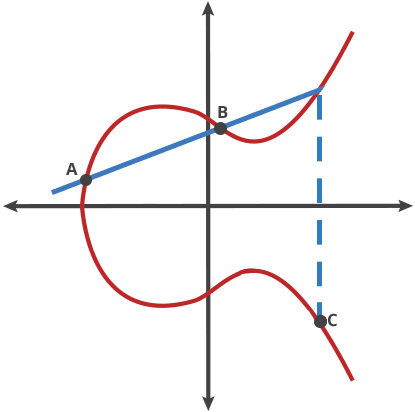
\includegraphics[width=0.35\textwidth]{ecc_2.png}
    \caption{Operation $\circ$ auf Punkten $A,B \in M$ \cite{ecc-cloud2013elliptic}}
    \label{fig:ecc_2}
\end{figure}

Die Operation $\circ$ kann beliebig oft hintereinander mit dem jeweils neu entstehenden Punkt ausgeführt werden. Genau hier liegt die Trapdoor function von ECC. Mit Kenntnissen über den Startpunkt $A$ und die Anzahl der Ausführungen $n$, ist es einfach den Endpunkt $E$ zu berechnen. Wenn allerdings nur der Endpunkt $E$ und der Startpunkt $A$ gegeben sind, ist es sehr rechenaufwändig die Anzahl an Ausführungen zu bestimmen.

\subsection{Vor- und Nachteile}
Allgemein liefert ECC eine schnellere Berechnungszeit als RSA \cite{ecc-mahto2018performance}. Da sich die Laufzeiten von Verschlüsselung und Entschlüsselung durch RSA und ECC asymptotisch nicht gleich verhalten, ist es schwer eine endgültige Antwort zu nennen. Allerdings schlägt ECC RSA bei der Gesamtzeit für Ver- und Entschlüsselung je nach Nachrichtengröße um einen Faktor von $\mathtt{\sim}3-20$ \cite{ecc-mahto2018performance, ecc-bao2022research}. Zudem eignet sich ECC vor allem als Ver- und Entschlüsselungsmethode auf rechenschwachen Geräten wie Mobiltelefonen aufgrund von kleineren Schlüsselgrößen\footnote{Um eine Bit Security Level von 256 Bits mit RSA zu erreichen, ist eine Schlüssellänge von 15360 Bits nötig, während es bei ECC lediglich 512 Bits sind.\cite{ecc-mahto2018performance}}. So können Rechenaufwand, Energieverbrauch und RAM-Auslastung gesenkt werden \cite{ecc-gupta2011ecc}.

Allerdings wurde 2007 bekannt, dass der Pseudozufallszahlengenerator ``Dual\_EC\_DRBG'' eine potenzielle Backdoor hat, die es Nutzern mit Informationen über einen geheimen Wert ermöglichte die Zufälligkeit problemlos zu knacken \cite{ecc-green2013backdoor}. Dual\_EC\_DRBG wurde 2005-2006 zusammen von NIST (National Institute of Standarts and Technology) und der NSA veröffentlicht und basiert die Auswahl der zurück gegebenen pseudozufälligen Zahlen auf Berechnungen über elliptischen Kurven. Dieser Vorfall schwächt bis heute das generelle Vertrauen in ECC. \cite{ecc-cloud2013elliptic}

\section{AES - Advanced Encryption Standard}
\label{sec:aes}
Der Advanced Encryption Standard ist einer der weltweit am häufigsten verwendeten symmetrischen Verschlüsselungsalgorithmen. AES wurde 2001 vom NIST als offizieller Standard für die Verschlüsselung von Daten festgelegt und hat den früher verwendeten Data Encryption Standard (DES) ersetzt, da dieser als unsicher galt. AES basiert auf dem Rijndael-Algorithmus, der von den Kryptographen Joan Daemen und Vincent Rijmen entwickelt wurde \cite{aes-jamil2004rijndael}. Die hohe Sicherheit, Effizienz und Flexibilität von AES haben dazu beigetragen, dass er heute in einer Vielzahl von Anwendungen, von vertraulichen Regierungsdokumenten, bis hin zur Verschlüsselung von Festplatten und Netzwerkverkehr zum Einsatz kommt.

AES ist ein blockbasierter Verschlüsselungsalgorithmus, der Daten in Blöcken von 128 Bit verarbeitet. Dabei verwendet AES symmetrische Schlüssel, was bedeutet, dass derselbe Schlüssel sowohl für die Verschlüsselung als auch für die Entschlüsselung der Daten verwendet wird. Der Algorithmus unterstützt Schlüsselgrößen von 128, 192 und 256 Bit, wobei größere Schlüssel im Allgemeinen eine höhere Sicherheit bieten, jedoch auch höhere Rechenressourcen erfordern. AES durchläuft mehrere Runden von Transformationen, die die Klartextdaten in scheinbar zufälligen Geheimtext umwandeln. Bei der 128-Bit-Schlüsselgröße umfasst der Algorithmus 10 Runden, bei 192-Bit sind es 12 Runden und bei 256-Bit werden 14 Runden verwendet. Jede dieser Runden besteht aus mehreren Schritten auf Bitmatrizen. Unter den in einer Runde angewandten Operationen sind Substitution (Byte Substitution mittels S-Box), Zeilenverschiebung, Spaltenmischung und das Hinzufügen eines Rundenschlüssels \cite{aes-abdullah2017advanced}.

Das zentrale Sicherheitsmerkmal von AES ist seine Widerstandsfähigkeit gegen bekannte Kryptoangriffe wie Differenzial- und Linearkryptoanalyse \cite{aes-de2019linear,aes-hameed2018review}. Dies wird durch eine starke Schlüsselabhängigkeit und die Nutzung mehrerer kryptographischer Prinzipien, wie der Substitutions-Permutations-Netzwerkstruktur (SPN), erreicht. Darüber hinaus spielt die sogenannte Avalanche-Eigenschaft eine entscheidende Rolle: Eine kleine Änderung im Klartext oder im Schlüssel führt zu drastischen Änderungen im Geheimtext, wodurch es Angreifern erschwert wird, Rückschlüsse auf den ursprünglichen Klartext oder den verwendeten Schlüssel zu ziehen \cite{aes-bhoge2014avalanche}.

Verglichen mit asymmetrischen Verschlüsselungsverfahren fehlen AES jedoch gewisse Schutzziele, die über die letzten Jahre zunehmend an Wichtigkeit gewonnen haben. Die Verwendung von einem einzelnen Schlüssel führt dazu, dass die Integrität einer Nachricht nicht sichergestellt werden kann, was bedeutet, dass Veränderungen an der Nachricht, die nicht vom ursprünglichen Sender, stammen nicht festgestellt werden können. Aus diesem Grund haben Sadi Arman, Shamim Al Mamun und Nuray Jannat einen modified AES Algorithmus (MAES) veröffentlicht, der durch die Verwendung weiterer Bit Verschiebeoperationen eine Senderauthentifizierung, Empfängerauthentifizierung und Nachrichtenintegrität gewährleisten kann \cite{aes-arman2024modified}. Der Algorithmus beschränkt die für AES üblichen Schlüssellängenauswahl von 128, 192 und 256-bit Schlüsseln auf ausschließlich 128-bit Schlüssel, erhöht dafür aber gleichzeitig die Datenübertragungsrate um bis zu 20\% \cite{aes-arman2024modified}.

\section{Abschluss}
%pro und contra von allen
Aus dieser Liste an verwandten Arbeiten geht hervor, dass es noch kein Bezahlsystem gibt, das den in Kapitel \ref{chap:req} aufgestellten Anforderungen gerecht wird. Die Tabelle \ref{tab:nichtfunktionale_Anforderungen} gibt dabei einen Überblick über die vorgeschlagenen Lösungsansätze und welche der Anforderungen durch sie nicht erreicht werden.
\begin{table}[H]
    \centering
    \begin{tabular}{|c|c|c|c|c|}
        \hline
        & GNU Taler & Bitcoin & Ethereum & Privacy Pass \\
        \hline
        Anonymität & $\times$  & $\mathtt{\sim}$ & $\mathtt{\sim}$ & $\checkmark$ \\
        \hline
        Unverkettbarkeit & $\checkmark$  & $\mathtt{\sim}$ & $\mathtt{\sim}$ & $\checkmark$ \\
        \hline
        Zeitsensitivität & $\checkmark$ & $\times$ & $\times$ & $\checkmark$ \\
        \hline
        Skalierbarkeit & $\checkmark$ & $\mathtt{\sim}$ & $\checkmark$  & $\checkmark$\\
        \hline
        Vertraulichkeit & $\checkmark$ & $\checkmark$ & $\checkmark$ & $\mathtt{\sim}$ \\
        \hline
        Integrität & $\checkmark$ & $\checkmark$ & $\checkmark$ & $\mathtt{\sim}$ \\
        \hline
    \end{tabular}\\
    \vspace{5pt}
    $\checkmark$: ist erfüllt; $\mathtt{\sim}$ ist teilweise erfüllt; $\times$ ist nicht erfüllt
    \caption{Erfüllung nichtfunktionaler Anforderungen}
    \label{tab:nichtfunktionale_Anforderungen}
\end{table}
GNU Taler erfüllt jede der Anforderungen -- abgesehen von der Anonymität. Zwar schützt GNU Taler die Anonymität des Käufers und hält dessen Privatsphäre aufrecht, allerdings sollte ein im DT-Modell verwendetes Bezahlsystem hauptsächlich die Privatsphäre des Verkäufers schützen, die von GNU Taler gezielt öffentlich gemacht wird.

Bitcoin und Ethereum teilen sich aufgrund der Verwendung einer Blockchain das Problem von nicht zeitsensitiven Transaktionsdauern. Mit einer geschätzten Wartezeit von einer Stunde bzw. sechs Minuten, bis eine Transaktion mit ausreichend Sicherheit bestätigt werden kann, ist die Verwendung der beiden Technologien unter Einhaltung der Anforderungen nicht möglich. Des Weiteren kann argumentiert werden, dass durch den Public Ledger, der alle Transaktionen pseudonymisiert veröffentlicht, die Anonymität und Unverkettbarkeit nur in Teilen gewahrt werden kann. 

Vertraulichkeit und Integrität werden durch Privacy Pass nicht nativ unterstützt. Da das Protokoll ausschließlich für das Umgehen von CAPTCHAs bei CDNs entwickelt wurde, ist von einer https-Verbindung auszugehen, die diese Schutzziele gewährleistet. Jedoch sieht Privacy Pass selbst keine Maßnahmen zum Schutz der Kommunikation vor.\\

Aufgrund dessen, dass keines der zuvor genannten Bezahlsysteme sämtliche Anforderungen erfüllt, muss für den Anwendungsfall im DT-Modell ein neues Bezahlsystem entworfen werden. Dieses Bezahlsystem wird in dem folgenden Kapitel genauer beschrieben und spezifiziert. 



%==================================================================================================



\chapter{Systementwurf}
\label{chap:systems}
In dem folgenden Kapitel werden die neu erarbeiteten Systeme genau beschrieben. Dafür werden zu Beginn einige Designentscheidungen und Ziele des Systems genannt. Anschließend wird für jedes der drei Systeme ein detailierter Ablauf beschrieben und weitere wichtige Informationen für die Funktionsweise der Systeme genannt.

\section{Ziel}
\label{sec:mainPart_ziel}
Um einen privatsphäreschützenden Anreiz für die Benutzung eines DTs zu schaffen wird im Folgenden ein Bezahlsystem vorgestellt. Dieses Bezahlsystem erlaubt es dem DG für den Handel mit seine Daten im Gegenzug einen finanziellen Ausgleich zu verlangen, ohne dabei persönliche Informationen -- ausgenommen der in den Daten enthaltenen Informationen -- preisgeben zu müssen. Weder der DN noch der DT kann bei einer regulären Transaktion bestimmen, welcher DG eine Bezahlung erhält. Der hierfür verwendete Ablauf sieht vor, dass ein DG zuerst seine Daten an den DN überträgt und ihm etwas Zeit zur Verwertung der Daten lässt. Sollte nach Ablauf der Zeit keine Bezahlung für den DG vorliegen, so kann der DT den DN von der weiteren Verwendung der Plattform ausschließen. 

Damit der DG seine Anonymität nicht ausnutzen kann, gibt es zwei Mechanismen zur Betrugserkennung. Der erste ist eine Offenlegung der Kommunikation im Streitfall. Sollte sich eine der beiden Parteien betrogen fühlen, so kann sie vom DT eine Schlichtung verlangen. Dafür wird für die Kommunikation ein Einmalschlüssel verwendet, der dem DT mitgeteilt werden kann, sodass dieser alle Schritte nachvollziehen kann. Anhand der übertragenen Nachrichten kann der DT entscheiden, ob ein Betrug vorliegt oder nicht. 
Der zweite Mechanismus ist ein Reputationssystem. Wenn ein DG qualitativ gute Daten liefert, kann ein DN eine gute Bewertung für ihn ausstellen, was seine Reputation verbessert. Wenn er hingegen schlechte Daten liefert, so kann ein DN eine schlechte Bewertung abgeben. Die -- durch die Bewertungen beeinflusste -- Reputation eines DG liefert dem DN vor Erwerb der Daten eine Einschätzung über die Qualität der Daten. Dafür kann bei jedem Aufruf nach Daten von einem DN ein Reputationsschwellwert festgelegt werden, um die Daten von DG mit zu schlechter Reputation von der Auswahl auszuschließen.

\section{Geld als Anreiz}
\label{sec:incentiveExplaination}
Zuerst wird geklärt warum Geld als Anreiz für den DG -- zum Teilen seiner Daten -- verwendet wurde. Da im Datentreuhandmodell ein DN meist durch ein Unternehmen oder eine Forschungseinrichtung repräsentiert wird, ist es vorstellbar, dass der DN selbst eine Dienstleistung anbieten oder in Aussicht stellen kann. Als Anreiz wurde hier jedoch Geld gewählt, da die Verwendung von -- durch den DN angebotenen -- Dienstleistungen als Anreiz einige Nachteile mit sich ziehen kann.

\begin{enumerate}
    \item \textbf{Universal.} Kein Handelsgut und keine Dienstleistung ist so universell begehrt wie Geld. Es ist möglich, das ein Business, welches hier als DN auftritt, für die Preisgabe der Daten eine Dienstleistung anbietet. Beispielsweise können Social Media Plattformen wie X kostenlose zeitlich bedingte Premiumabonnenments oder vergleichbare Angebote in Aussicht stellen. Jedoch ist das Interesse an solchen Angeboten subjektiv, was sie als mögliche Anreize zwar denkbar aber eher suboptimal macht.
    \item \textbf{Einheitlich.} Wenn der Anreiz zum Teilen von Daten durch den DN gestellt wird, wird das Angebot von jedem einzelnen DN unterschiedlich sein. Aus der Kommunikationsstruktur folgt, dass alle unterschiedlichen Kompensationen auf irgendeinem Weg über den DT laufen müssen. Daraus ergibt sich ein großer zusätzlicher Aufwand an Entwicklung und Implementation für jeden DN.
    \item \textbf{Verfügbarkeit.} Manche DN, wie beispielsweise Forschungsinstitutionen, haben nur eine eingeschränkte Auswahl an Dienstleistungen oder Produkten die sie DG anbieten können. Da sie hauptsächlich an der Forschung interessiert sind, verfügen sie über erheblich weniger Konsum- oder Unterhaltungsprodukte verglichen mit anderen Firmen. Geld ist hingegen deutlich leichter zugänglich.
    \item \textbf{Wahrung der Anonymität.} Viele C2B Treuhänder legen Wert auf die Anonymität oder Pseudonymität der DG. Diese kann jedoch dadurch, dass ein DN die versprochene Dienstleistung kontrolliert, verloren gehen. Es ist beispielsweise denkbar, dass ein DN einen vielversprechenden Anreiz verspricht, diesen aber hinter einer Registrierung und Angaben von persönlichen Daten verbirgt, so dass die durch den Treuhänder etablierte Anonymität umgangen wird.
    \item \textbf{Einhalt der Leistung.} Der DT kann bei der Auslagerung von Anreizen an den DN nicht zuverlässig kontrollieren, dass der DN die versprochene Dienstleistung wirklich einhält.
\end{enumerate}
Durch die Verwendung von Geld als Anreiz können diese Punkte leichter eingehalten werden. Die Wahl der DG ist nun ausschließlich abhängig von dem Ruf und dem persönlichen Interesse an dem DN und nicht von dessen Anreizangebot. Der Anspruch auf den versprochenen Anreiz ist für jeden DN gleich implementiert und hängt nur von unterschiedlichen Preisen ab. Es kann davon ausgegangen werden, dass alle DN über Geld verfügen und dieses als Kompensation verwenden können. Aufgrund des Stellenwertes von Geld in der Gesellschaft sind bereits viele Wegen entwickelt worden, wie dessen Wert anonym oder pseudonym an andere übertragen werden kann. Einige davon wurden bereits in den Abschnitten \ref{subsec:gnu}, \ref{sec:bitcoin} und \ref{sec:ethereum} genannt. Abschließend behält der DT die volle Kontrolle darüber, dass ein zu zahlender Geldbetrag vom DN abgegeben wird und auch bei dem richtigen DG ankommt.

\section{Annahmen über das Datentreuhandmodell}
\label{sec:systemAssumptions}
Ein DT kann in verschiedenen Variationen eingesetzt werden. Abschnitt \ref{sec:dt} gibt darüber bereits einen Überblick. Im Folgenden werden Annahmen getroffen, die das DT-Modell betrefen, für welches das Anreizsystem entworfen wird. Dadurch soll verdeutlicht werden, in welchem DT-Modell das System am besten eingesetzt werden kann.

Zuerst sei anzunehmen, dass es sich bei dem DT um einen freiwilligen C2B Treuhänder handelt. Dies ist dadurch begründet, dass bei verpflichtenden DTs die Benutzung vorgeschrieben ist und daher ein Anreiz zur Benutzung des Systems irrelevant für die Nutzerzahlen ist. Weiter haben bei Business to Business Treuhändern beide Parteien einen Profit aus dem Tausch der Daten. Beide sind gleichzeitig am Daten empfangen und am Daten versenden. Hier fällt daher eine deutliche Einteilung in DG, die Anreize erhalten und DN, die Anreize bieten, schwer. 

Die beim DT abgelegten Daten sind verschlüsselt. Der DT speichert lediglich eine lange Liste an Bytes, kann aber anhand der verschlüsselten Bytes nicht feststellen, was die Daten beinhalten, welche Daten von welchem DG stammen oder wo ein Datensatz aufhört und der nächste beginnt. Er weiß also nichts über die bei ihm abgelegten Daten. Damit ein DG trotzdem den Zugang zu seinen Daten behält, werden ihm beim Hochladen seiner Daten Werte für den konkreten Ablageort seiner Daten, sowie einen passenden Schlüssel zur Entschlüsselung mitgeteilt. Wenn er seine abgelegten Daten nun einsehen möchte, kann er den Satz an Bytes von dem Speicherort anfragen und den erhaltenen Geheimtext mit Hilfe des Schlüssels entschlüsseln, was seine ursprünglich hochgeladenen Daten zum Vorschein bringt.

Es gibt zwei Paradigmen wie DN die passenden DG auswählen und von ihnen Daten beziehen. In dem ersten Paradigma bietet ein DG seine Daten zum Verkauf beim DT an. Daraufhin kann ein DN diese Daten anfordern, auswerten und anschließend bezahlen. Im zweite Paradigma erstellt der DN einen Aufruf zum Teilen von Daten. Dieser Aufruf hat einen bestimmen Datentyp und Informationen über den DN. Nun kann sich ein DG einen passenden Aufruf heraussuchen und seine Daten an den DN weiterleiten. \\
Im Folgenden wird vom zweiten Paradigma ausgegangen, da es sowohl Rechenaufwand- als auch Privatsphärenvorteile liefert. Das Erstellen eines Aufrufs sowie das Weiterleiten zum DT sollte beides in $O(1)$ geschehen. Das Erstellen eines Aufrufs beinhaltet nur die Zusammensammlung von Informationen wie Datentypen, Namen oder Beschreibung. Es sind in der Regel keine iterativen Vorgänge aktiv, die die Laufzeit in $O(n)$ bringen könnte. Im Anschluss sind keine weiteren Berechnungen von Nöten, um Daten zu empfangen. Bei der individuellen Auswahl von DG und der Nachfrage nach deren Daten entsteht hingegen ein Zusammenhang zwischen der Anzahl an Datensätzen und des Rechenaufwands des DN. Da der DN für jeden DG eine Bewertung erzeugen muss, die darüber entscheidet, ob die Daten erworben werden oder nicht, ergibt sich für den Erhalt von $n$ Datensätzen ein Rechenaufwand von $O(n)$. Die Minimierung des Rechenaufwands für den DN ist vor allem interessant, da DN durch Unternehmen repräsentiert werden, die in Extremfällen mehrere tausend Anfragen pro Sekunde bearbeiten müssen, während DG an ihren Endgeräten einen deutlich überschaubareren Rechenaufwand leisten müssen. \\
Privatsphärenvorteile werden durch das zweite Paradigma ebenfalls erbracht, da die Einreichung von Daten so vollständig anonym ablaufen kann. Solange durch die Kommunikation zur Mitteilung des Speicherorts und Datenschlüssels keine Informationen preisgegeben werden, kann der DN den DG unmöglich deanonymisieren. Die von ihm erhaltenen Datenparameter können dazu benutzt werden, Daten beim DT zu erfragen. Dieser weiß genauso wenig, wessen Daten angefragt wurden. Im ersten Paradigma hingegen müssen mindestens die Informationen, die ein DN braucht, um eine aussagekräftige Einschätzung über die Daten trefen zu können, bereitgestellt werden. Je nach dem welche Informationen davon betroffen sind, besteht eine Möglichkeit, die Angebote eines DG miteinander zu verlinken und so Informationen über ihn zu gewinnen.

 

\section{Geheimhaltung der Identitäten}
%PKI für schlüssel assumen
Im Gegensatz zu GNU Taler soll das Bezahlsystem hauptsächlich den DG und dessen Informationen schützen. Die Privatsphäre des DN ist zwar ebenfalls schützenswert, aber eher von geringerer Bedeutung, da im DT-Modell der DN meist durch ein Unternehmen oder eine Forschungseinrichtung dargestellt wird. Hinzu kommt die Struktur eines DTs, die den DN dazu veranlasst, eine Menge an Informationen anzugeben, um vom DT zugelassen zu werden. Der DG hingegen ist eine einzelne Privatperson, die ihre gesammelten Daten bewusst an Unternehmen oder Forschungseinrichtungen verkaufen möchte. Der Schutz der Privatperson ist hier daher von größerem Interesse. 

Unter diesen Umständen ist eine herkömmliche Überweisung per Bank deutlich zu unsicher. Sie benötigt Informationen wie die IBAN des belasteten Kontos und die IBAN des empfangenden Kontos, um zu wissen, von wo nach wo eine Geldsumme fließen soll. Dadurch werden bereits zu viele Informationen über den DG bekannt, da der DN nun genau herausfinden kann, von wem die erworbenen Daten stammen und ob er bereits vorher schon von demselben DG Daten gekauft hat. Dies entspricht einem Ziel der in Kapitel \ref{chap:req} definierten Angreifermodelle. Zusätzlich kann die Bank -- als ``außenstehender Angreifer`` -- nachvollziehen, dass eine Privatperson sich als DG angemeldet und welchem DN sie ihre Daten bereits verkauft hat.\\
Um dieses Problem zu lösen, wird hier eine der gängigsten anonymen Onlinezahlmethoden verwendet: Kryptowährungen. Die Abschnitte \ref{subsec:gnu}, \ref{sec:bitcoin} und \ref{sec:ethereum} führen bereits einige davon auf und beschreiben, warum diese unter Anwendung der Anforderungen nicht im DT-Modell benutzbar sind. Aufgrund dessen wird hier ein neues System eingeführt. Jedoch sind dessen Coins weder Blockchain basiert, noch für Spekulationszwecke brauchbar. Ein Coin kann -- so wie bei vielen Kryptowährungen üblich -- ausschließlich bei einem Exchange (EX) gegen Geld getauscht werden. Bei dem initialen Tauschen mehrerer Coins ist der monetäre Wert in Euro fest im Coin gespeichert und kann nicht verändert werden. 

Es gibt keine Regulierung oder Identifizierungspflicht zum Erwerb von Coins, doch nur DN können sicher Coins ausgeben, da das Bezahlsystem nur Transfers von DN zu DG erlaubt. DG können Coins zwar erwerben, jedoch können diese nur außerhalb des Systems -- wo kein Betrugsschutz greift -- getauscht werden. Da Coins vor dem Tausch nicht auf Echtheit geprüft werden können ist anzunehmen, dass nur DN Coins erwerben werden, da der Tausch unter DG deutlich zu unsicher ist.

\section{Verschlüsselung}
Da in der Kommunikation indirekt Geld transferiert wird, ist es von höchster Priorität, die gesendeten Nachrichten vor dem Mithören oder Verändern durch unbefugte Dritte zu schützen. Dies wird zusätzlich sowohl durch die in Kapitel \ref{chap:req} definierten Angreifermodelle, als auch durch die Anforderungen vorrausgesetzt. Für diesen Schutz wird eine Mischung aus der in Abschnitt \ref{sec:ecc} erklärten elliptischen Kurven Kryptographie und dem in Abschnitt \ref{sec:aes} angeführten MAES-Algorithmus verwendet. 

Mit der Benutzung eines PKs bei ECC wird sichergestellt, dass nur Personen mit Wissen über den zugehörigen SK die Nachricht lesen können. Anschließend wird ein Hashwert der verschlüsselten Nachricht gebildet und mit dem SK des Senders signiert. Auf diesem Weg kann der Empfänger der Nachricht selbst den Hash bilden und prüfen, ob der signierte Hash mit dem selbst gebildeten übereinstimmt. Dadurch kann sowohl die Vertraulichkeit als auch die Integrität der Nachricht sichergestellt werden.

AES hingegen verwendet nur einen Schlüssel, der gleichzeitig zum Verschlüsseln und Entschlüsseln einer Nachricht gebraucht wird. Es erreicht erheblich schnellere Berechnungszeiten als ECC, da AES auf Operationen basiert, die lediglich Bits verschieben, aber keine komplexen mathematischen Berechnungen durchführen. Da AES aber keine Integrität gewährleisten kann, wird hier für die symmetrische Kommunikationsverschlüsselung der MAES-Algorithmus verwendet. Durch ihn kann -- wie bei ECC -- eine unbemerkte Veränderung der Nachricht ausgeschlossen werden.

Damit der andere Gesprächspartner an den PK zum Überprüfen der Signatur gelangt, wird angenommen, dass es eine Public Key Infrastructre (PKI) gibt, die zuverlässig den jeweiligen PK auf Anfrage herausgibt. An einigen Stellen der folgenden Protokolle ist es jedoch essentiell, einen neuen unbekannten PK zu verwenden, damit die kommunizierende Person nicht wiedererkannt werden kann. An diesen Stellen wird sowohl TLS als auch ein Proxy verwendet, um die Kommunikation sowohl anonym, als auch vertraulich und sicher vor Veränderungen zu gestalten. Alle folgenden Nachrichtentupel, für die keine Verschlüsselung spezifiert ist, sind ECC für Vertraulichkeit und Integrität geschützt.

\section{Coin Generierungsphase}
\label{system:coingeneration}
Hier werden die Coins, die im späteren Verlauf beider Systeme verwendet werden, vom DN erstellt und vom DT signiert. Die einzelnen Schritte sind in Abbildung \ref{fig:coin-generationphase} verdeutlicht und werden im Folgenden beschrieben. Dafür werden alle einzelnen Schritte des Protokolls jeweils ein kurzer Absatz formuliert, der die Operationen des Nachrichtenempfängers beschreibt. Zusätzlich steht neben der Nummerierung der Protokollschritt ein Tupel aus den -- in dieser Nachricht übertragenen -- Informationen.
\subsection{Ablauf}

\paragraph*{Gestrichelte Pfeile} $([a,b]), ([e])$\\
Die Pfeile zwischen 4. und 5. sind hier gestrichelt eingetragen, da sie notwendige Kommunikationsschritte von partiell blinden Signaturen abbilden. Sie sind essenziell für deren Funktionsweise und wurden bereits in \ref{sec:partBlindSig} erklärt, weshalb sie hier nur zur Vollständigkeit aufgelistet werden.

\begin{figure}[H]
    \centering
    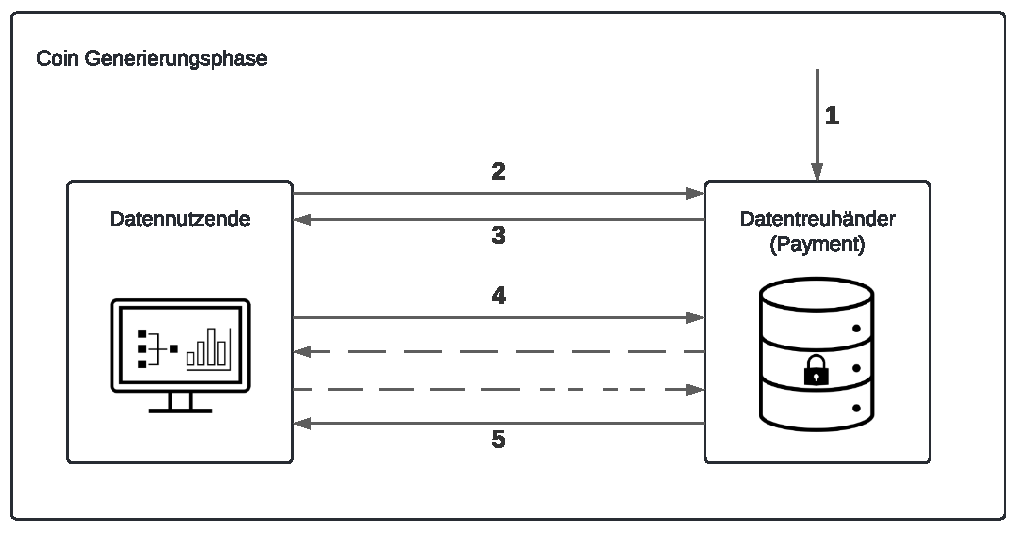
\includegraphics[width=0.7\linewidth]{CoinGenerationPhaseDiagramm.pdf}
    \caption{Coin Generierungsphase Ablauf}
    \label{fig:coin-generationphase}
\end{figure}

\paragraph{1. Zahlungseingang} $(APK, ES)$\\
Der EX erhält über einen beliebigen Weg eine $ErhaltenenSumme$ $(ES)$ und einen $AccountPublicKey$ $(APK)$. Die genaue Umsetzung des Zahlungseingangs liegt bei dem EX. Er kann alles zwischen einer Banküberweisung mit dem $APK$ als Verwendungszweck, bis hin zu einem Briefumschlag mit Bargeld und einem leserlich aufgeschriebenen $APK$ sein. Nach Eingang einer Zahlung erstellt der EX einen sogenannten $CoinGenerationToken$, bestehend aus $(nonce, APK, ES, spent \leftarrow false)$, verschlüsselt ihn mit dem $APK$ und speichert diesen intern. Der $nonce$ ist dabei eine zufällig gewählte große Zahl, die den Token einmalig macht. Der $CoinGenerationToken$ wird verschlüsselt, da sonst jede andere Person, die den $APK$ mitgeschnitten hat, selbst den Token verwenden kann, um Coins für sich zu generieren.

\paragraph{2. CoinGenerationToken abrufen} $(APK)$\\
Da der EX nur den $APK$ erhält, hat er keine Möglichkeit den $CoinGenerationToken$ einem DN zuzuweisen. Jetzt kann jeder beliebige Nutzer alle Einträge für einen $APK$ abfragen. Allerdings ist nur der DN in der Lage den $CoinGenerationToken$ zu entschlüsseln, der den passenden SK zum $APK$ hat. Dies ist im Idealfall nur der DN, der die Transaktion getätigt hat. Dafür überträgt der DN den $APK$ und fragt nach allen gespeicherten Token, die diesen $APK$ beinhalten. Da der $APK$ ein öffentlicher Schlüssel ist, kann der DN ihn für die Signatur und fortfolgende Kommunikation nutzen.

\paragraph{3. CoinGenerationToken übertragen} $([\{nonce, APK, ES\}_{APK}])$\\
Auf eine $CoinGenerationToken$ Anfrage des DN antwortet der EX mit allen noch nicht eingelösten Token für den $APK$. Nachdem der DN die Token erhalten hat, kann er diesen zuerst mit dem passenden SK entschlüsseln. Im Anschluss kann er selbst Coins erstellen. Ein Coin besteht aus $(nonce, value)$. Der $nonce$ ist hier wieder eine zufällig gewählte große Zahl. Bei der Erstellung sind zwei Sachen zu beachten: Zuerst muss die Summe über alle $value$ gleichgroß sein wie die $ES$ des Tokens. Des Weiteren gibt es eine Menge an möglichen Werten $MW$, sodass $\forall value\in MW$ gilt. Dies ist vor allem wichtig, da $value$ beim Signieren und Einlösen des Coins für den EX sichtbar ist und dieser bei einer Wahl eines selten vorkommenden $value$ eine Verbindung zwischen den Phasen herstellen kann.

\paragraph{4. Signierung Anfragen} $((nonce, APK, ES), [value])$\\
Eine Signieranfrage ist der Start eines Durchlaufs von partiell blinden Signaturen, bestehend aus einem $CoinGenerationToken$ und einer Menge an $values$. Zuerst kann der EX prüfen, ob der gesendete Token noch nicht eingelöst wurde. Anschließend summiert er alle $value$ auf und prüft, ob die Summe gleich dem $ES$ des Tokens ist. Wenn beide dieser Überprüfungen akzeptieren, kann der EX mit dem partiell blind signieren anfangen und bei seinem gespeichert Token $spent \leftarrow true$ setzen um eine doppelte Einlösung zu verhindern.

\paragraph{5. Signieranfrage Antwort} $([r,c,s,d], \pi_{sk})$ \\
Vorausgesetzt, alle Überprüfungen aus Schritt 4 werden akzeptieren, so erhält der DN nun eine Menge an partiell blind signierten Coins und kann diese für die spätere Verwendung lokal speichern. Zusätzlich berechnet der EX einen BDLEQ, wie er in \ref{sec:privacy-pass} beschrieben ist. Nachdem der DN diesen verfiziert hat, kann er sicher sein, dass der EX zum signieren seiner Coins den selben SK, verwendet hat wie für die Signatur aller Coin Generierungsphasen mit anderen Nutzern. Sollten die Überprüfungen nicht akzeptieren, so kann der DN entweder bei Schritt 4 mit anderen Coins, oder bei Schritt 2 wieder ansetzen.\\

Auf diese Weise kann ein DN Geld bei einem EX einzahlen und eine dem Geldbetrag entsprechende Menge an Coins erhalten, ohne dass der EX die von ihm ausgehändigten Coins oder den DN nachverfolgen kann. Gleichzeitig ist es für einen DN nicht möglich, Coins zu erhalten, für die er keinen monetären Gegenwert bereitgestellt hat.

\subsection{Finanzierung des Exchange}
Zusätzlich ist zu erwähnen, dass EX finanziell motiviert sein können und eine Gebühr verlangen möchten, um beispielsweise laufende Serverkosten zu decken. Sollte dies der Fall sein, kann vor dem Beginn der Coin Generationsphase vom EX eine feste Gebühr kommuniziert werden. Wenn sich ein DN trotz der Gebühr dazu entscheidet diesen EX zu verwenden, so kann der EX nach dem Eingang einer Zahlung in Schritt 1 einen $CoinGenerationToken$ erstellen, welcher die Gebühr bereits abzieht. Wenn also ein DN eine Transaktion von $100$\texteuro\ bei EX mit $10\%$ Gebühr tätigt, so erstellt der EX einen $CoinGenerationToken$ für den angegebenen $APK$ mit $ES \leftarrow 90$\texteuro. Auf diese Weise kann ein EX seine finanziellen Interessen geltend machen. 

\section{Bezahlvorgang}
\label{system:payment}
Nachdem die Coins erstellt und signiert sind, kann das Ausgeben dieser Coins behandelt werden. Dafür gibt es das Bezahlsystem, welches dem DN erlaubt die Daten von DGs anzufragen. Diese können der Anfrage nachkommen, wofür sie der DN im Gegenzug mit den Coins entlohnt. Damit bei dem Vorgang die Privatsphäre des DG so gut wie möglich geschützt wird, findet der Austausch der Daten und Coins über Postfächer beim DT statt. Dadurch entsteht keine direkte Kommunikation zwischen DG und DN, die potenziell schützenswerte Informationen wie IP-Adresse oder dergleichen preisgibt. Wie der Ablauf genau funktioniert, wird im Folgenden erklärt. Hier werden wieder die einzelnen Protokollschritte beschrieben und deren übertragene Daten mit Tupeln verdeutlicht.

\subsection{Ablauf}
\begin{figure}[H]
    \centering
    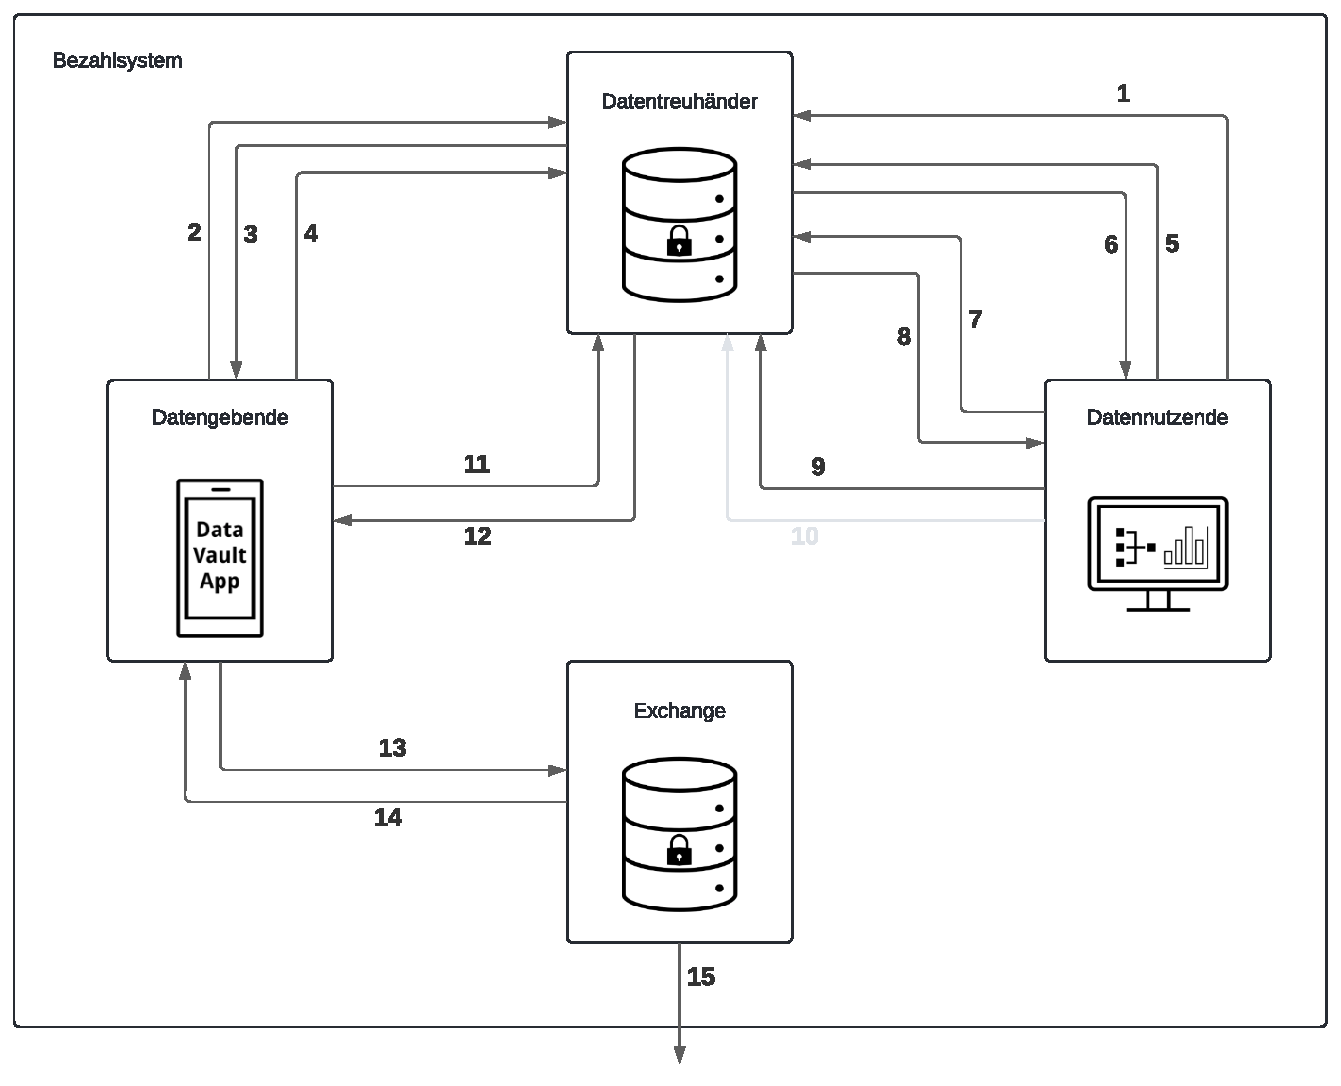
\includegraphics[width=0.9\linewidth]{PaymentDiagramm.pdf}
    \caption{Bezahlsystem Ablauf}
    \label{fig:payment}
\end{figure} 

In der Abbildung \ref{fig:payment} sind die Pfeile mit den Nummern 7,8 und 11 grau markiert. Dies hat den Grund, dass das Diagramm den gesammten Kommunikationsfluss zeigt und diese drei Schritte nur für das Bewertungssystem relevant sind, welches in Abschnitt \ref{system:reputation} beschrieben wird. Deswegen folgt die Auflistung und Erklärung der übertragenen Informationen erst in Abschnitt \ref{system:reputation}.

\paragraph{1. Aufruf starten} $(CallDetails, DataType, Price, Call$-$PK)$\\
Der DN erstellt beim DT einen Aufruf zur Datenteilung. Damit verkündet er an alle DG, dass er Daten von einem bestimmten Typ sucht und benennt direkt, wieviel er bereit ist für diese Daten zu bezahlen. Der $Call$-$PK$ kann von einem DN für jeden Aufruf vergeben werden. Er hilft bei der Organisation und Zuordnung von später folgenden Datenpostfacheinträgen zu Aufrufen. Die genauen Inhalte der $CallDetails$ sind Treuhänderabhängig, da je nach Gebiet des Treuhänders verschiedene Details über den DN für die Entscheidung des DG wichtig sein können. In den meisten Fällen umfassen die $CallDetails$ Daten wie einen Titel, den Namen des DN, eine Beschreibung oder den Verwendungszweck der gesammelten Daten. Auch Informationen darüber, ob es sich bei dem DN um eine Forschungseinrichtung handelt, können hier kommuniziert.

\paragraph{2. Aufrufliste anfragen} $()$\\
Damit ein DG über die Liste an allen aktuell laufenden Aufrufen bescheid weiß, muss er diese Liste beim DT anfragen. Es werden hier vorerst keine Informationen benötigt, da solange das Reputationssystem nicht in Kraft ist, jeder DG gleich gestellt ist und Einsicht auf die vollständige Liste an Aufrufen erhält.

\paragraph{3. Aufrufliste Antwort} $([CallDetails, DataType, Price, Call$-$PK])$\\
Nachdem der DG die Aufrufliste angefragt hat, kann der DT seine lokale Datenbank mit Aufrufen sammeln und alle Aufrufe in eine Liste aufnehmen. Damit enthält jeder Eintrag der Liste einen Aufruf der wie in Schritt 1 beschrieben aus $CallDetails$, dem gesuchten $DataType$, dem dafür ausgeschriebenen $Price$ und dem vom DN verwendeten $Call$-$PK$ besteht. Diese Liste an Aufrufen wird an den DG zurück gesendet werden.

\paragraph{4. Daten teilen} $(Call$-$PK, \{SHK\}_{Call-PK}, \{ReferenceCode, DataLocation, DataKey\}_{SHK})$\\
Der DG hat die genannten Aufrufdetails erhalten und sich dazu entschieden, seine Daten für einen Aufruf mit einem DN zu teilen. Generell gilt wie in Abschnitt \ref{sec:systemAssumptions} erklärt, dass ein DG seine Daten nicht selbst speichert, sondern sie verschlüsselt beim DT lagert. Er behält nur den Speicherort und Schlüssel der Daten, um jederzeit Zugriff auf diese zu haben. Um seine Daten mit einem DN zu teilen, genügt es daher den Speicherort und Schlüssel zu übertragen.

Für die Übertragung des Speicherorts und Schlüssels wird ein Postfach beim DT verwendet. So kann ein direkter Austausch zwischen DG und DN verhindert werden. Ein DG kann Ort und Schlüssel verschlüsselt in das Postfach legen und nur der DN, der das Wissen über den passenden privaten Schlüssel besitzt, kann Ort und Schlüssel wieder entschlüsseln.

Einer der Betrugserkennungsmechanismen ist die Offenlegung der Kommunikation im Streitfall, so dass der DT die Nachrichten einsehen und entscheiden kann, welche der Parteien recht behält. Damit bei dieser Offenlegung nur genau die Nachrichten entschlüsselt werden, die Teil einer spezifischen Kommunikation zwischen DG und DN sind, wird für jede Abwicklung eines Tausches ein neuer symmetrischer Schlüssel $SHK$ erstellt.

Damit ein DG einen Eintrag in das Postfach zum Teilen von Daten senden kann, muss er zuerst die folgenden Informationen bestimmen. Zuerst wird der $Call$-$PK$ des DN im Klartext angegeben. So kann ein DN beim Abfragen des Postfaches bestimmen, welche Einträge für ihn verschlüsselt sind. Anschließend wird ein neuer symmetrischer Schlüssel $SHK$ erstellt. Dieser wird mit dem $Call$-$PK$ verschlüsselt, damit nur der DN den $SHK$ kennt. Nun kann der DG den $SHK$ verwenden um das Tupel aus $DataLocation$, $DataKey$ und $ReferenceCode$ zu verschlüsseln. Die $DataLocation$ und $DataKey$ sind der eben beschriebene Speicherort und Schlüssel. Dabei sei angemerkt, dass sowohl $DataLocation$, als auch $DataKey$ mehr als nur eine Variable sein können und von dem vom DT verwendeten Speicher- und Verschlüsselungsverfahren abhängen. Der $ReferenceCode$ ist eine zufällige Zahl, die später bei Schritt 13 verwendet wird, um die Coins für diesen Postfacheintrag abzufragen.

\paragraph{5. Datenpostfach abfragen} $(Call$-$pk)$\\
Der DN kann sich zu einem beliebigen Zeitpunkt dazu entscheiden, alle Nachrichten, die den angegebenen $Call$-$PK$ enthalten, anzufragen. Dafür muss er den gewünschten $Call$-$PK$ mitübertragen, um dem DT zu signalisieren, an welchen Nachrichten er Interesse hat. Der $Call$-$PK$ muss hier bei jeder Anfrage spezifiziert werden, da ein DT keine Liste über die von einem DN erstellten Aufrufe führt und daher nicht alle Nachrichten für alle $Call$-$PK$ eines DN zusammenfassen kann.

\paragraph{6. Datenpostfach Antwort} $([\{SHK\}_{Call-pk}, \{ReferenceCode, DataLocation, DataKey\}_{SHK}])$\\
Nachdem der DT die Anfrage an das Datenpostfach erhalten hat, erstellt er eine Liste mit Postfacheinträgen, die den $Call$-$PK$ der Anfrage im Klartext angegeben haben. Die einzelnen übertragenen Postfacheinträge können dabei auf den $Call$-$PK$ verzichten, da dieser nur zur Identifizierung genutzt wird. Der DN kennt den $Call$-$PK$ ohnehin, da er ihn in der Anfrage definiert. Die vollständige Liste aller Postfacheinträge kann zurück an den DN gesendet werden.

\paragraph{9. Daten anfragen} $(DataLocation)$\\
Der DN kann nun für jeden empfangenen Postfacheintrag den passenden SK verwenden, um den $SHK$ des Eintrags zu entschlüsseln. Solange der DG sich an das Protokoll gehalten und den Schlüssel, den er zum Verschlüsseln des $SHK$ verwendet hat auch als Klartextschlüssel angegeben hat, funktioniert dieser Schritt einwandfrei und der DN erhält Zugang zu $SHK$. Mit diesem kann er das Datentupel aus $DataLocation$, $DataKey$ und $ReferenceCode$ entschlüsseln. Jetzt kann er den DT nach den Daten an der angegebenen $DataLocation$ fragen, welche mit dem $DataKey$ verschlüsselt sind.

\paragraph{10. Daten Antwort} $(\{data\}_{DataKey})$\\
Die durch die $DataLocation$ beschriebenen Daten werden durch den DT ausgelesen. Da auch hier wieder keine Authentifizierung stattfindet, kann jeder einen beliebigen Datensatz beim DT anfragen und erhält die an der Stelle gespeicherten Daten. Da allerdings nur der DN, der die $DataLocation$ und den $DataKey$ vorher erhalten hat, die Daten lesen kann, ist das wahllose Anfragen von Daten beim Treuhänder sinnlos. Ohne Wissen über die $DataLocation$, kann es zu Anfragen von teilhaften Datensätzen oder Überlappungen in andere Datensätze kommen. Der DT kann zwar bei einer Anfrage nachvollziehen, von welchem DN diese kommt, aber kann nicht bestimmen welchem DG die Daten gehören und kann daher auch keinen Handel zwischen DG und DN feststellen.

Nach Erhalt der verschlüsselten Daten kann der DN den zu den Daten gehörenden $DataKey$ verwenden, um die Daten zu entschlüsseln und an den Klartext zu gelangen. Jetzt kann der DN die Daten für seine Zwecke verwerten.

\paragraph{12. Coins in Postfach legen} $(ReferenceCode, \{[nonce,value]\}_{SHK})$\\
\label{para:payment_9}
Mit der abgeschlossenen Verwertung kann der DN nun den DG bezahlen. Dafür lädt er eine Liste an Coins aus seinem Speicher, die in der Summe gleich dem im Aufruf ausgeschriebenen Preis sind. Er verwendet den in Schritt 6 erhaltenen $SHK$ um die Liste an Coins zu verschlüsseln. Anschließend verwendet er den ebenfalls in Schritt 6 erhaltenen $ReferenceCode$, um einen Eintrag an das Coinpostfach zu senden.

Da der $ReferenceCode$ von dem DG mit dem $SHK$ verschlüsselt wurde, ist davon auszugehen, dass ein Eintrag mit dem gleichen $ReferenceCode$ nur von dem DN stammen kann, der den Aufruf gestartet und die Daten erhalten, entschlüsselt und verwertet hat.

\paragraph{13. Coinpostfach abfragen} $(ReferenceCode)$\\
Da ein DG nach dem Erstellen eines Datenpostfacheintrags den dort genutzten $ReferenceCode$ lokal als ``noch nicht bezahlt'' abspeichert, kann er bei Bedarf den DT fragen, ob es bereits einen Eintrag in dem Coinpostfach mit diesem $ReferenceCode$ gibt. Er kann somit den DT fragen, ob er für das Teilen seiner Daten bereits bezahlt wurde.

\paragraph{14. Coinpostfach Antwort} $(\{[nonce,value]\}_{SHK})$\\
Wenn der DN bereits einen Eintrag mit den verschlüsselten Coins eingesendet hat, so werden die unter dem $ReferenceCode$ angegebenen verschlüsselten Coins an den DG zurückgegeben. Der DG kann daraufhin den $SHK$, welcher in Kombination mit dem $ReferenceCode$ gespeichert wurde, verwenden, um die erhaltenen Coins wieder zu entschlüsseln. Wenn er anschließend die Liste an Coins erhält, kann er überprüfen, ob die Summe der Coins den Preis des Aufrufs ergibt und die partiell blinde Signatur, die in der Coin Generierungsphase Schritt 4. und 5. ausgestellt wurde, tatsächlich valide ist. Sollten diese Tests beide akzeptieren, so kann der DG die Coins lokal speichern, bis er sie einlösen möchte.

\paragraph{15. Coins einlösen} $([nonce,value], Addresse, DG-ID, \{DG-ID\}_{DT-sk})$\\
Ein DG kann seine angesammelten Coins jederzeit einem EX senden. Dafür kann er die in Schritt 14 gespeicherten Coins aus dem Speicher lesen und gesammelt oder einzeln an einen EX übertragen. Um bösartiges Verhalten des DN vorzubeugen, wird die ID des DG zusammen mit einer Signatur dieser vom DT zum Einlösen der Coins benötigt. Durch diese Signatur wird sichergestellt, dass ein DG tatsächlich seine eigene ID angibt und diese nicht beliebig durchtauschen kann. Ohne die $DG-ID$ kann ein DN eine Menge an Coins übertragen und selbst wieder einlösen, bevor der DG die Chance dazu erhält. Zusätzlich wird eine Form einer Zahlungsadresse -- oben $Addresse$ -- zum EX gesendet. Bei der Implementation wird das Übertragen einer IBAN verwendet, allerdings ist es genauso gut möglich stattdessen eine Bitcoin Walletadresse oder eine beliebige andere Zahlungsmöglichkeit zu verwenden. Ein EX kann auch mehrere Zahlungsoptionen gleichzeitig anbieten. In dem Fall muss die Zahlungsoption als zusätzlicher Parameter mit übertragen werden.

\paragraph{16. Bestätigung} $([nonce, message])$\\
Nachdem die Coins beim EX eingetroffen sind, überprüft dieser, ob die Coins bereits vorher schon eingelöst wurden und ob die partiell blinde Signatur gültig ist. Nachdem alle Tests durchgelaufen sind, generiert er eine Liste, die für jeden $nonce$ eine $message$ speichert. Für diese $message$ gibt es vier Möglichkeiten. Wenn die Tests der Doppelausgabe und partiell blinde Signaturen akzeptieren, so wird $\{``ok``\}$ in die $message$ geschrieben. Wenn die Validierung der partiell blinden Signatur fehlschlägt, so wird $\{``blindSig\_validation\_failed``, nonce, \{``blindSig\_validation\_failed``, nonce\}_{EX-sk}\}$ in die $message$ geschrieben. Fällt beim überprüfen auf, dass der Coin bereits von einem anderen DG eingelöst wurde, so wird $\{``already\_spent``, nonce, \{``already\_spent``, nonce\}_{EX-sk}\}$ in die $message$ geschrieben. Falls der Coin von dem selben DG vorher eingelöst wurde, ist die $message$ nur $\{``error\_with\_spending``\}$. Anschließend wird die Liste mit allen $nonce$ und deren $messages$ zurück an den DG gesendet.

\paragraph{17. Geld austeilen} $(address)$\\
Hier wird abschließend eine ausgehende Zahlung vom EX zu der angegebenen Zahlungsadresse in Höhe aller vollständig eingelösten Coins getätigt. Die genau kommunizierten Daten sind hier von der Zahlungsoption abhängig. Allerdings muss hier sichergestellt werden, dass der ausgehende Betrag genau dem Wert der eingelösten Coins gleicht.

\subsection{Verwendung von Proxys und TLS}
Damit eine Unverkettbarkeit der Anfragen gewährleistet werden kann, müssen die Anfragen der Protokollschritte 4,7,12 und 13 vollständige anonym gesendet werden. Dafür kann ein Proxy genutz werden. Die Aufgabe des Proxys ist hier die Verschleierung der IP-Adresse. Durch das Weiterleiten durch einen Proxy bleibt die wahre IP-Adresse des DG bzw. DN geheim. Ohne diesen Proxy kann der DT über die IP-Adresse mehrere Nachrichten miteinander verbinden und über längere Zeit mitschneiden, welcher DG oder DN an wie vielen Handeln beteiligt war. Tatsächlich ist eine dauerhaft gleichbleibende IP-Adresse eine Seltenheit. Der IPv4 Adressraum ist bereits seit mehreren Jahren erschöpft \cite{tls-huston2008changing}, weshalb IPv4 Adressen in regelmäßigen Abständen neu an aktuell sendende Geräte verteilt werden \cite{tls-jin2007identifying}. Trotzdem bleibt die IP-Adresse für mindestens eine Sitzung mit dem DT gleich, was diesem ermöglicht, alle in dieser Sitzung gesendeten Nachrichten zu der selben Person zurückzuverfolgen. 

Die Art oder der Anbieter des Proxys ist in diesem Kontext nicht von Bedeutung. Solange er zuverlässig eingehende Nachrichten an die angegebene Ziel-IP-Adresse weiterleitet, bleibt die wahre IP-Adresse geschützt, was dem DT keine Möglichkeit zur Verlinkung mehrerer Nachrichten lässt.\\

Durch den Proxy wird die Identität des Sendenden versteckt. Deshalb muss eine alternative Herangehensweise für die Gewährleistung von Integrität eingesetzt werden, da der DT nun nicht mehr den PK des Sendenden einsehen kann. Dafür kann die Kommunikation in den Schritte in denen ein Proxy verwendet, über TLS ablaufen. Das Transport Layer Security Protokoll (kurz TLS) ermöglicht es einem Nutzer, mit einem Server zu kommunizieren und die dabei übertragenen Nachrichen gegen das Lesen und Veränderung durch Dritte zu schützen \cite{tls-brumbaughssl}. Dafür benötigt TLS keinen PK des Senders, sondern handelt bei jeder Verbindung einen neuen Schüssel aus \cite{tls-Arfaoui2019The}. So kann die Integrität aller Nachrichten eingehalten werden, während der Server die Identität des Sendenden nicht verlinken kann. TLS verwendet standartmäßig RSA zur Verschlüsselung. Es kann jedoch alternativ durch ECC ersetzt werden wie in \cite{tls-ecc-blake2006elliptic} beschrieben wird. Dadurch können erhebliche Performanzsteigerungen erzielt werden \cite{tls-ecc-koschuch2012price}.

\subsection{Bezahlungszeitraum}
\label{subsec:paymentTimespan}
Ein häufiger Betrugsversuch im Onlinehandel ist das Vortäuschen einer Zahlungsintention durch den Käufer, die nicht eingehalten wird. Hier trifft dies den Fall, in dem ein DN einen Aufruf startet; DG in dem Vertrauen bezahlt zu werden ihre Daten weitergeben und der DN mit den gesammelten Daten verschwindet. Um DG vor diesem Fall abzusichern, gibt es einen Maximalbezahlraum von 12 Stunden. Sollte also ein DG innerhalb von 12 Stunden nach dem Weiterleiten seiner Daten keine Bezahlung erhalten, so hat er die Möglichkeit beim DT eine Beschwerde einzureichen. Wenn die Schuld tatsächlich beim DN liegt und dieser keine Zahlung nachweisen kann, kann der DT den DN nach wiederholtem Vorkommen dauerhaft von der weitergehenden Benutzung der Plattform ausschließen. Da zur Registrierung als DN in der Regel eine große Menge an Informationen wie Name, Branche, Verwendungszweck der Daten, etc. anzugeben sind, kann angenommen werden, dass sich ein DN nach dem Ausschluss nicht einfach unter einem anderen Namen wieder registrieren kann. Außerdem wird in dem Paper \cite{roebert2024unlinkable} von K. Röbert, A. See, J. Schug und M. Fischer ein Verfahren präsentiert, dass es ermöglicht, Nutzer -- selbst nach Änderung ihres Namens -- eindeutig wieder zu erkennen. Dieses Verfahren kann hier eingesetzt werden um sicherzustellen, dass kein DN ,der bereits von der Verwendung ausgeschlossen wurde, sich erneut registrieren kann.\\

Die Dauer von 12 Stunden kann von Treuhänder zu Treuhänder variieren. Dieser Zeitraum wurde gewählt, um einem bösartigen DN keine zu große Menge an Daten stehlen zu lassen, bevor seine Machenschaften bemerkt werden. So steigt beispielsweise die Menge an Daten, die der DN stehlen kann, linear mit dem Bezahlungszeitraum, solange davon ausgegangen wird, dass der Andrang an DG, die ihre Daten teilen, zeitlich gleichverteilt ist. Gleichzeitig sollte der Zeitraum nicht zu klein gewählt sein, da eine Nichteinhaltung schwerwiegende Folgen hat. Bei einer Wahl von wenigen Sekunden reicht z.B. ein Serverausfall des DN, um den Bezahlzeitraum zu überschreiten, ausreichend Beschwerden zu sammeln und einen Ausschluss auszulösen.

\subsection{Mögliche Streitfälle}
\label{subsec:payStreit}
Wie schon bei \ref{sec:mainPart_ziel} erwähnt wurde, sollen im Streitfall die Kommunikationsschritte, die den Austausch von Daten und die dazugehörige Bezahlung beinhalten, offengelegt werden können. Wie genau diese Offenlegung funktioniert und in welchen Fällen sie benutzt wird, wird hier geschildert.\\

\begin{enumerate}
    \item \textbf{Fehlerhafte Verschlüsselung.}\label{case:IncorrectEncryption}
    Der erste Streitfall kann nach Schritt 6 entstehen. Zu diesem Zeitpunkt hat der DG bereits die $DataLocation$ und den $DataKey$ mit dem $SHK$ verschlüsselt, in das Postfach des DTs gesendet und der DN hat diesen Eintrag erhalten. Sollte nun der DN den erhaltenen Eintrag nicht entschlüsseln können, so liegt dies entweder an einem inkorrekt angewendeten, angegebenem oder übertragenen $Call$-$PK$ oder $SHK$. Da der Eintrag anonym in das Postfach beim DT abgelegt wurde, besteht vorerst keine Möglichkeit für den DN Maßnahmen zu ergreifen. Erst nach Ablauf der 12 Stunden, nach denen sich der DG beschwert, dass er keine Coins erhalten hat, kann eine Lösung gefunden werden. Der DG verweist auf den Eintrag, der mit Hilfe des $SHK$ verschlüsslt wurde und legt den $SHK$ offen. Der DT kann probieren den Eintrag mit Hilfe des $SHK$ zu entschlüsseln. Sollte es ihm nicht gelingen, liegt die Schuld beim DG. Wenn es ihm doch gelingt, so erhält der DN eine Chance zu zeigen, dass er den $SHK$ nicht lesen konnte. Dafür wird der $SHK$ mit dem im Eintrag gespeicherten $Call$-$PK$ verschlüsselt. Sollte dabei ein unterschiedlicher Geheimtext entstehen als in dem Eintrag unter $\{SHK\}_{Call-PK}$ abgelegt ist, so wurde falsch verschlüsselt. Stimmen die Geheimtexte überein, so ist anzunehmen, dass der DN sowohl den Schlüssel als auch die Daten lesen kann und die Bezahlung verweigert. 

    Für diese Beweisstruktur ist essenziell, dass die asymmetrische Verschlüsselung mittels ECC bei Verwendung der selben Parameter den selben Geheimtext ausgibt. Dies ist nicht selbstverständlich, da für die Verschlüsselung häufig Techniken wie das Salten (hinzufügen einer Zufallsvariable) verwendet werden, um jedes Mal einen unterschiedlichen Geheimtext zu erhalten.
    
    
    \item \textbf{Fehlerhafte Datenparameter.}\label{case:IncorrectDataParameters}
    Dieser Fall tritt nach Schritt 10 ein. Der DN hat die unter $DataLocation$ abgelegten Daten erhalten, kann jedoch nach entschlüsseln dieser mithilfe des $DataKey$ nur unleserliche Geheimtexte erhalten. Auch hier wird der $SHK$ und der Postfacheintrag dem DT mitgeteilt. Dieser kann sich durch das Entschlüsseln Zugang zur $DataLocation$ und zum $DataKey$ verschaffen. Daraufhin überprüft er selbst, ob er die unter $DataLocation$ abgelegten Daten mit dem $DataKey$ entschlüsseln kann. Erhält er dabei ebenfalls nur unleserliche Geheimtexte, so ist die angegebene Kombination aus $DataLocation$ und $DataKey$ inkorrekt und die Schuld liegt beim DG. Sollte er jedoch leserliche Daten vorfinden, wird dies als Betrugsversuch des DN gewertet.

    \item \textbf{Nutzlose Daten.}\label{case:UselessData}
    Ähnlich wie Punkt \ref{case:IncorrectDataParameters} tritt dieser Streitfall nach Schritt 10 auf. Hier kann der DN die referenzierten Daten zwar lesen, empfindet diese jedoch als nutzlos. Das Vorgehen zur Offenlegung deckt sich ebenfalls mit dem von Punkt \ref{case:IncorrectDataParameters}. Der DN gibt Postfacheintrag und $SHK$ an, der DT entschlüsselt den Eintrag, liest die Daten von der $DataLocation$ und entschlüsselt diese mit dem $DataKey$. Es gilt nun abzuwägen, ob die vorliegenden Daten tatsächlich nutzlos sind. Diese Bewertung ist in den meisten Fällen schwer zu entscheiden. Sollte es sich um einen völlig leeren Datensatz handeln, der nur aus Nullbits besteht, kann mit überwiegender Sicherheit angenommen werden, dass die Daten tatsächlich nutzlos sind. Andernfalls müsste der DT selbst die Mechanismen zur Auswertung der Daten besitzen. Wie in \ref{sec:dt} genannt wurde, besitzen eine Vielzahl an DTs die Möglichkeit eine Qualitätssicherung der Daten durchzuführen. Dadurch kann ein DT die Qualität der Daten begründet einschätzen und entscheiden, ob der DN mit seiner Behauptung recht behält. Sollte der DT keine Qualitätssicherung liefern können oder sich bei der Beurteilung unsicher sein, wird im Zweifel für den DG entschieden.

    \item \textbf{Fehlerhafte Coins.}\label{case:IncorrectCoins}
    Ein Streitfall aufgrund fehlerhafter Coins kann sowohl in Schritt 14 als auch in Schritt 16 eintreten. Im Fall von Schritt 14 hat der DG gerade seine Bezahlung aus dem Coinpostfach des DTs abgeholt. Daraufhin hat er die partiell blinde Signatur des EX überprüft und festgestellt, dass die für den Coin angegebene Signatur nicht valide ist. Um den DT darüber aufzuklären, leitet er den $SHK$, $ReferenceCode$ und $Call$-$PK$ weiter und lässt den DT die Signatur prüfen. Wenn der DT anerkennt, dass die abgelegte Signatur ungültig ist, kann er den angegebenen PK mit der Liste an Aufrufen abgleichen und den zu dem Aufruf gehörenden DN bestrafen.\\
    
    Ein Coin kann genauso erst in Schritt 16 als fehlerhaft erkannt werden. Sollte die Signaturüberprüfung durch den DG in Schritt 14 ohne Probleme ablaufen, sendet er die Coins anschließend an den EX. Dieser wiederholt das Prüfen der Signatur. Da diese Validierung bereits in Schritt 14 reibungslos ablief, ist davon auszugehen, dass auch hier keine anderen Ergebnisse entstehen. Trotzdem kann ein Coin erst beim Einlösen an dem EX auf doppelte Ausgabe überprüft werden. Sollte der EX feststellen, dass ein übermittelter Coin zu einem vorherigen Zeitpunk schon einmal eingelöst wurde, so verhält er sich wie in Schritt 16 spezifiert und sendet ein signierte Auskunft über den Coin zurück zum DG. Daraufhin kann der DG diese signierte Auskunft dem DT zusammen mit dem $SHK$ und dem $ReferenceCode$ vorzeigen. Der DT entschlüsselt den Coinpostfacheintrag und prüft, ob der $nonce$ der Auskunft in der Nachricht enthalten ist. Findet er den $nonce$ vor, so kann er unter betracht der signierten Auskunft des EX davon ausgehen, dass der DN zwei DG mit dem gleichen Coin bezahlen wollte und ihn entsprechend bestrafen.

    \item \textbf{Überschreitung des Bezahlzeitraums.} \label{case:paymentExceeded}
    Wie schon in \ref{subsec:paymentTimespan} erläutert, hat der DG nach einer Wartezeit von 12 Stunden die Möglichkeit, eine Beschwerde beim DT einzureichen. Dafür speichert er beim Absenden eines Eintrags zum Datenpostfach die Zeit und fragt in beliebigen Abständen das Coinpostfach nach dem $ReferenceCode$ ab. Sollte 12 Stunden nach absenden des Eintrags noch keine Antwort vorliegen, so leitet er den $SHK$ zusammen mit dem Datenpostfacheintrag an den DT. Dieser validiert, dass der DG tatsächlich seine Daten geteilt hat und prüft, ob bereits ein Eintrag unter dem $ReferenceCode$ eingesendet wurde. Trifft dies nicht zu, wird das Handeln des DN als Verstoß gegen die Einhaltung des Bezahlzeitraums gewertet und entsprechend bestraft.
\end{enumerate}


\section{Reputationsvergabe}
\label{system:reputation}
Nach Erhalt der Daten soll der DN in der Lage dazu sein, eine Bewertung für den DG aufgrund seiner Daten auszustellen. Erneut gilt es hier die Privatsphäre des DG weitgehend zu schützen. Dafür erhält der DN zusammen mit der $DataLocation$ und $DataKey$ einen Bewertungstoken, mit dem er eine Bewertung für die Qualität der Daten beim DT einreichen kann. Der DT kennt die Reputation jedes DG und ist für die Verwaltung, sowie regelmäßige Neuberechnung des Wertes zuständig.\\
In der Diskussion in Abschnitt \ref{sec:discussion} wird ein alternativer Ansatz besprochen. Er basiert auf einem Nachweis von bereits erhaltenen Coins durch den DG. Dort werden auch die Vor- und Nachteile dessen erklärt, sowie Gründe genannt, weshalb das aktuelle Konzept preferiert wird.

Das Bezahl- und Reputationssystem werden getrennt beschrieben obwohl deren Abläufe in einem Diagramm zu sehen sind. Dies hat den Grund, dass das Bezahlsystem auch alleinstehend -- ohne Reputationssystem -- verwendet werden kann. Da durch das Streitfallsystem bereits eine Maßnahme zum Schutz vor Betrug besteht, gibt es -- obwohl es trotzdem empfohlen wird -- keine Verpflichtung das Reputationssystem mit zu implementieren. Im Folgenden werden alle Erweiterung genannt die anfallen, wird das Reputationssystem verwendet. Dafür wird erneut der Nachrichteninhalt als Tupel hinzugefügt.
\subsection{Ablauf}
\begin{figure}[h]
    \centering
    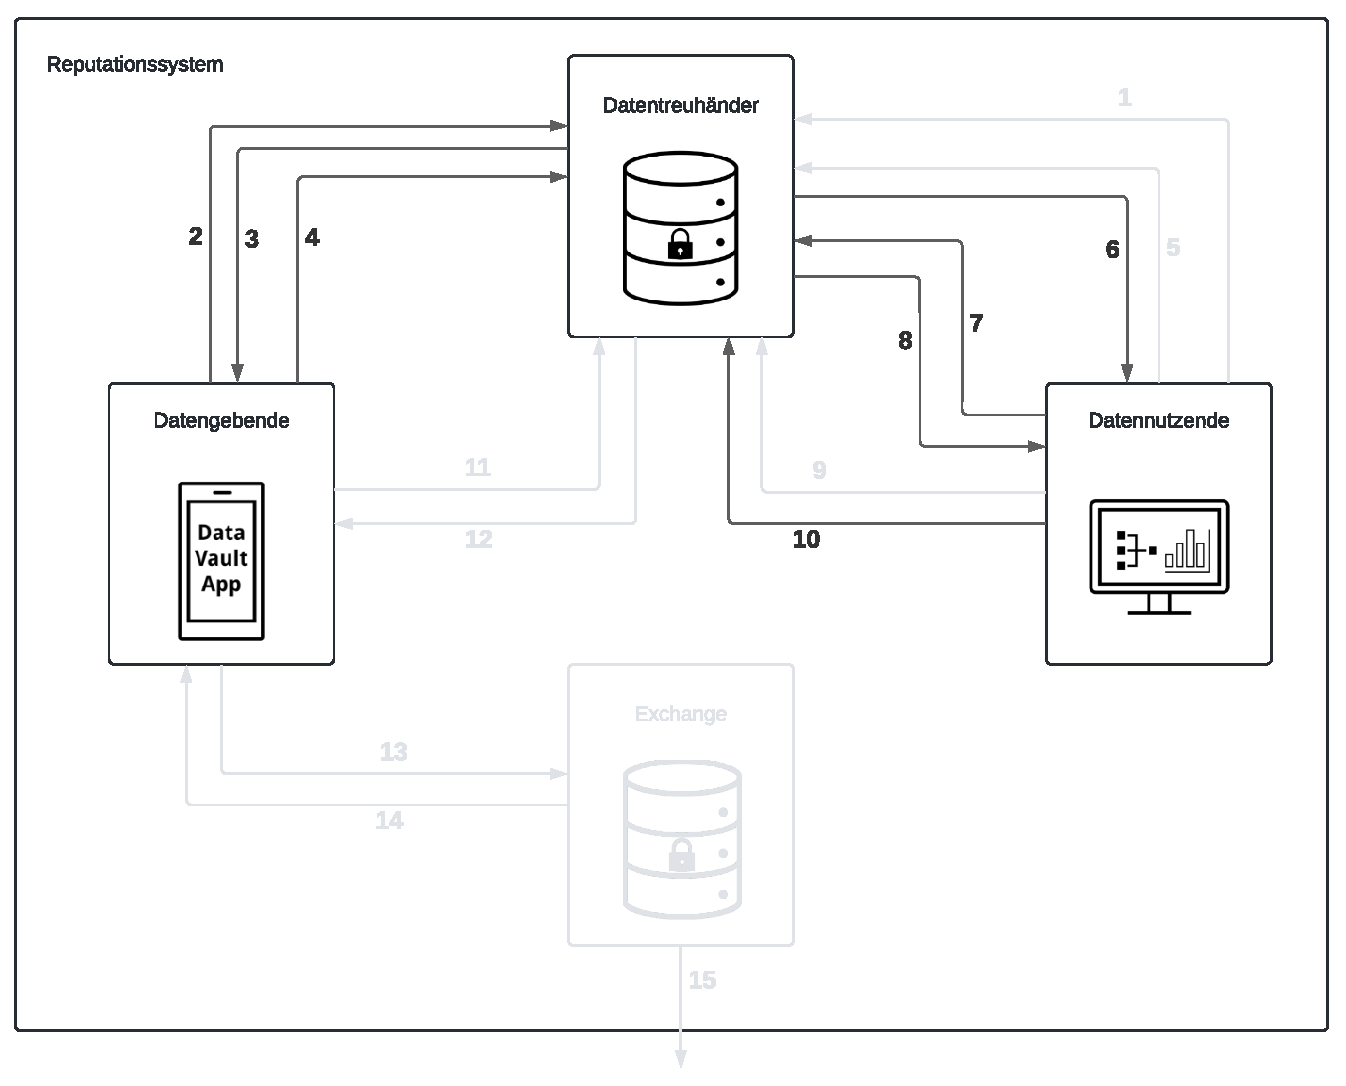
\includegraphics[width=0.9\linewidth]{ReputationDiagramm.pdf}
    \caption{Reputationssystem Ablauf}
    \label{fig:reputation}
\end{figure}

Auch in Abbildung \ref{fig:reputation} werden wieder nur die für das Bewertungssystem relevanten Kommunikationsschritte hervor gehoben. Die grauen Schritte sind Teil des Bezahlsystems und in \ref{system:payment} dokumentiert. 

\paragraph{1. Aufruf starten} $(ReputationThreshold)$\\
Das Starten eines Aufrufs wird durch die Verwendung des Reputationssystems leicht abgewandelt. Die in Abschnitt \ref{system:payment} beschriebenen $CallDetails$, $DataType$, $Price$ und $Call$-$PK$ bleiben bestehen. Hinzu kommt die Angabe eines $ReputationThreshold$. Dieser legt fest, dass nur DGs mit einer Reputation über diesem Schwellwert Zugriff auf diesen Aufruf erhalten. DGs deren Reputation unterhalb des Schwellwertes ist, bleiben von der Einsendung ihrer Daten ausgeschlossen.


\paragraph{2. Aufrufliste anfragen} $(DG-ID, {\{DG-ID\}}_{DG-SK})$\\
Beim Abfragen der Aufrufliste muss nun eine signierte $DG-ID$ mitgesendet werden. Die Signatur kann durch den DT überprüft werden. Damit wird sichergestellt, dass sich ein DG nicht unter anderer ID melden kann. Stimmt die Signatur der ID, so kann der DT die Reputation des DG aus seiner Datenbank laden und die Liste an Aufrufen damit filtern. Anschließend kann er nur die Aufrufe zurück geben, dessen $ReputationThreshold$ unterhalb der Reputation liegt. Um die Anfrage vor Replayangriffen zu schützen wird bei der Signatur ein Saltwert hinzugefügt. Dieser sorgt dafür, dass die Signatur einmalig ist.

\paragraph{4. Bewertungstoken mitsenden}$(RatingToken \leftarrow (nonce, {\{DG-ID\}}_{DT-pk},\\{\{nonce, {\{DG-ID\}}_{DT-pk}\}}_{DG-sk}))$\\
Beim Teilen von Daten kann ein DG einen Bewertungstoken erstellen. Dafür generiert er zufällig einen $nonce$ der Sicherstellt, dass Bewertungen nicht doppelt eingereicht werden können. Anschließend verwendet er den PK des DTs, um damit seine $DG-ID$ zu verschlüsseln. Dabei muss ein Saltwert hinzugefügt werden, da sonst bei jedem Verschlüsseln der ID der gleiche Geheimtext entsteht. Dadurch könnte ein DN den Ursprung von zwei Bewertungstoken verfolgen, was die Privatsphäre der DG verletzt. Abschließend berechnet der DG eine Signatur über den zufälligen $nonce$ und die verschlüsselte $DG-ID$. Sie stellt sicher, dass ein DN nicht selbst $nonce$ generiert und mehrere Bewertungen für eine $DG-ID$ einreicht oder die $DG-ID$ nach erhalt des Token ändert. Mit diesen drei Werten ist der Bewertungstoken vollständig und wird zusammen mit der $DataLocation$ und dem $DataKey$ an das Datenpostfach vom DT gesendet. Der Bewertungstoken wird dafür Teil des Textes, der mit dem $SHK$ verschlüsselt wird.

\paragraph{6. Bewertungstoken erhalten}$(RatingToken)$\\
Nach der Abfrage des Datenpostfachs in Schritt 5 erhält der DN die mit dem $SHK$ verschlüsselten Informationen über die Datenspeicherung beim DT, sowie den Bewertungstoken. Aufgrund der im Bewertungstoken übertragenen Details kann der DN kaum Überprüfungen auf dem Token durchführen. Er kann lediglich den verwendeten $nonce$ auf Wiederholungen überprüfen, um sicherzustellen, dass er nicht zwei Mal den gleichen Token erhalten hat. Die Signatur von $nonce$ und ${\{DG-ID\}}_{DT-pk}$ benötigt zwar zur Validierung nur den PK des DG, aber da die $DG-ID$ verschlüsselt ist und im Postfacheintrag der PK des DG nicht mitgesendet wird, kann der DG den nötigen PK nicht bestimmen. Daher bleibt ihm in diesem Moment nur die Möglichkeitm dem DG und dem überwiesenen Bewertungstoken zu vertrauen und auf die Bewertung des Tokens durch den DT in Schritt 11 zu warten.

\paragraph{7. Reputation abfragen}$({\{DG-ID\}}_{DT-pk})$\\
Den soeben erhaltenen Bewertungstoken kann der DN verwenden, um die darin gespeicherte verschlüsselte $DG-ID$ an den DT zu senden. Er selber kann die ID nicht lesen. Da sie mit dem PK des DTs verschlüsselt ist, muss sie an ihn weitergeleitet werden, um eine Aussage über die Reputation zu treffen. Dieser Schritt muss seperat von den Anfragen der Daten geschehen. Andernfalls weiß der DT, dass die gefragten Daten durch den gleichen DG hochgelanden wurden, dessen Reputation zurückgegeben werden soll.

Dieser Schritt ist nicht essentiell für das Protokoll und kann bei Bedarf auch weggelassen oder zu einem späteren Zeitpunkt ausgeführt werden. In dem Fall, dass ein DN keinen großen Wert auf die Korrektheit aller Reputationswerte legt und möglicherweise in seiner Rechenleistung beschränkt ist, kann dieser Schritt und damit zusammen auch Schritt 8, übersprungen werden. Dadurch kann der DN zwei Kommunikationsschritte sparen. Ein Ansatz, in dem ein DN nur bei herausstechend schlechten Daten die Reputation des DG anfragt, ist beispielsweise genauso denkbar.

\paragraph{8. Reputation Antwort}$(Reputation)$\\
Der DT kann die $DG-ID$ problemlos entschlüsseln. Anschließend kann er die Reputation des DG aus seiner Datenbank auslesen und den Wert an den DN zurücksenden. Wie der genaue Wertebereich der Reputation definiert ist, hängt von der konkreten Implementation ab. In der Implementation in Kapitel \ref{chap:impl} ist der Wertebereich für eine Reputation $r$ zwischen $0\leq r\leq 1$. Sollte ein DG das erste Mal abgefragt werden, so kann der DT -- gegebenenfalls, dass die $DG-ID$ tatsächlich existiert -- einen neutralen Wert von hier $0,5$ zurückgeben. Auf diesem Weg erfährt der DN die Reputation des DG, ohne herausfinden zu können, mit welchem DG er handelt.

\paragraph{11. Bewertung einreichen}$(RatingToken, rating, {\{DN-Certificate\}}_{DT-sk})$\\
Nachdem der DN eine Bezahlung in das Coinpostfach gesendet hat, hat er die Möglichkeit eine Bewertung für die Qualität der Daten abzugeben. Im Gegensatz zum Übertragen von Coins ist das Abgeben einer Bewertung nicht verpflichtend. Es kann genauso wie Schritt 7 bei durchschnittlicher Qualität der Daten ausgelassen werden um die Performanz zu steigern. 

Um eine Bewertung einzureichen, sendet der DN ein Tripel aus dem Bewertungstoken, der Zufriedenheit mit den Daten und einem DN-Zertifikat an den DT. An dem Bewertungstoken hat sich nichts verändert. Er beinhaltet nach wie vor einen $nonce$, die verschlüsselte $DG-ID$ und die Signatur über diese beiden Werte. Nun kann der DN einen Wert festlegen, der seine Zufriedenheit mit den Daten repräsentiert. Dafür muss ein passender Wert aus dem gewählten Wertebereich bestimmt werden. Für das DN-Zertifikat wird angenommen, dass es bei der Registrierung eines DN beim DT ausgestellt wird. Es beinhaltet keine Informationen über den jeweiligen DN, sondern dient in dieser Situation ausschließlich dazu sicherzustellen, dass ein DG sich nicht selbst bewerten kann. 

Das Zertifikat ist optimal durch alternative Beweisformen austauschbar die zeigen, dass es sich bei der bewertenden Person um einen DN handelt, ohne dabei anzugeben welcher DN es ist. Denn wenn der DT bei einer Bewertung den DN bestimmen kann, so hat er ein direktes Indiz für den Handel zwischen dem DN und dem bewerteten DG.

Sobald das Tripel beim DT eintrifft, überprüft dieser ebenfalls den $nonce$ auf wiederholtes Vorkommen und stellt mithilfe des Zertifikates sicher, dass es sich bei dem Bewerterenden um einen DN handelt. Anschließend entschlüsselt er die $DG-ID$, ruft den ihm bekannten PK des entsprechenden DG ab und nutzt ihn, um die Signatur über den $nonce$ und die verschlüsselte $DG-ID$ zu validieren. Sollten alle diese Überprüfungen ohne Fehler ablaufen, so kann der DT sicher sein, dass der Token tatsächlich durch den angegebenen DG erstellt wurde und ein DN ihn für die Bewertung von genau diesem DG benutzt. Er speichert die erhaltene Bewertung zusammen mit der $DG-ID$ lokal ab bis der Reputationswert des DG das nächste Mal neu bestimmt wird. Dies kann nach jeder Bewertung, in regelmäßigen Zeitabständen oder beim nächsten Anfragen von Aufrufen geschehen. Dafür kann der DT für jeden DG, dessen aktuelle Reputation und sämtliche Bewertungen seit der letzten Berechnung verwenden, um damit eine neue Reputation zu erhalten. Wie die Gewichtung der unterschiedlichen Bewertungen verläuft, ist hier wieder nicht genau vorgegeben. In Kapitel \ref{chap:impl} wird ein mögliches Beispiel genannt.


\subsection{Weitere Streitfälle}
\label{subsec:repStreit}
Das Reputationssytem bietet weiteres Potenzial für Streitfälle, die durch die hier hinzukommenden Nachrichtenteile entstehen können. Im folgenden sind diese Streitfälle aufgelistet.
\begin{enumerate}
    \item \textbf{Kein/Doppelter Bewertungstoken.} \label{case:badRepToken}
    Nachdem der DN in Schritt 6 den Datenpostfacheintrag entschlüsselt hat, prüft er den Bewertungstoken auf Existenz sowie Einzigartigkeit. Sollte dabei auffallen, dass entweder kein Bewertungstoken vorhanden ist oder dieser Token zuvor bereits erhalten wurde, so kann der DN dieses Verhalten melden. Er liefert dem DT den $SHK$, mit dem er den Datenpostfacheintrag entschlüsseln kann. Stellt der DT ebenfalls einen Fehler mit dem Bewertungstoken fest, so erlaubt er den DN die Bezahlung auszulassen. Meldet sich der DG nach Ablauf von 12 Stunden und fragt nach seiner Bezahlung, kann der DT ihn auf sein Fehlverhalten hinweisen und entsprechend bestrafen.
    \item \textbf{Zu niedrige Reputation.} \label{case:insufficientRep}
    Wenn dem DN nach entschlüsseln des Bewertungstokens und Anfragen der Reputation auffällt, dass der DG nicht dazu berechtigt sein sollte auf den Aufruf zu antworten, legt er wieder den $SHK$ offen. Der DT kann die $DG-ID$ des Datenpostfacheintrags verwenden um zu überprüfen, ob der DG in der Lage sein sollte, den Aufruf zu sehen. Ist die Reputation des DG unter dem Reputationsschwellwert des in dem Datenpostfacheintrag referenzierten Aufrufs, so muss der DG den Aufruf entweder von einer veralteten Aufrufliste haben oder ein anderer DG mit ausreichender Reputation hat eine Liste von aktuellen Aufrufen öffentlich gemacht. Auch hier ist der DN nicht mehr dazu verpflichtet einen Eintrag in das Coinpostfach einzutragen, da der DG unrechtmäßig einen Aufruf beantwortet hat.
    \item \textbf{Inkorrekte Signatur.} \label{case:badSignature}
    Im Anschluss an das Einreichen einer Bewertung in Schritt 11 wird die Signatur des Bewertungstokens durch den DT überprüft. Sollte dabei ein Fehler entstehen, so wird zuerst der DN beschuldigt, die verschlüsselte $DG-ID$ ersetzt zu haben. Um diese Anschuldigung aufzuklären, legt er den $SHK$ offen. Der DT entschlüsselt den Datenpostfacheintrag und prüft, ob die Signatur des übertragenen Token bereits fehlerhaft ist. Stellt sich der übertragene Token als intakt heraus, so hat der DN versucht die $DG-ID$ des Tokens zu verändern und so eine Bewertung für einen anderen DG auszustellen. Dafür kann ihn der DT temporär sperren. Ist der übertragene Token jedoch ebenfalls fehlerhaft, so ist ein Fehler bei der Erstellung der Signatur entstanden. Dieser kann sowohl unwissentlich -- durch das falsche Signieren von korreken Werten -- als auch wissentlich -- durch das absichtliche Verwenden einer anderen verschlüsselten $DG-ID$ -- auftreten. Da die $DG-ID$ bewusst durch einen bösartigen DG ausgetauscht worden sein kann, muss mit der Bestrafung abgewartet werden. Zuerst soll der DN wieder die Bezahlung auslassen. Auf die Nachfrage des DG nach seiner Bezahlung kann die wahre ID bestimmt und eine Bestrafung festgelegt werden.
\end{enumerate}

\subsection{Bewertungsfrequenz verschleiern}
\label{sec:ratingObfuscation}
Der DT kennt zwar die Reputation eines jeden DG, allerdings soll er dessen Handelspartner oder Frequenz nicht anhand der Bewertungen erschließen können. Leider ist dies sehr einfach, da der DT jede Bewertung einem DG zuordnen muss. Auch wenn nicht jeder DN eine Bewertung für jeden Handel mit einem DG ausstellen muss, lässt sich so für den DT trotzdem ein ungefähres Bild des Engagements eines DG bilden. Deswegen wird davon ausgegangen, dass es eine Instanz gibt, die sich als DN beim DT registriert, aber kein Interesse an Daten hat. Sie ist ausschließlich dazu da, um Verschleierungsbewertungen abzugeben. Dafür kann sie wie ein regulärer DN einen Aufruf starten. Die DG übertragen jedoch keine Daten an den DN sondern lediglich einen Bewertungstoken. Dieser wird dazu verwendet, eine Bewertung auszustellen, die mit der aktuellen Reputation übereinstimmt, sodass sich bei Neuberechnung der Reputation kein Unterschied ergibt. Dadurch kann ein DG beliebig viele Bewertungen ausstellen, die seine Reputation nicht verändern und dadurch seine tatsächliche Handelsfrequenz gegenüber dem DT verschleiern. Nun kann der DT beim Erhalt einer Bewertung für einen DG nicht sicher sein, dass wirklich ein Handel stattgefunden hat, was die Privatsphäre des DG weiter stärkt.\\

Einige der in den Abschnitten \ref{subsec:payStreit} und \ref{subsec:repStreit} beschriebenen Streitfälle müssen für diesen speziellen Fall anders evaluiert werden. Beispielsweise ist hier der DG im Unrecht, wenn er 12 Stunden nach Absenden des Tokens den Streitfall \textit{Überschreitung des Bezahlzeitraums} ausruft, da er keine Daten geteilt hat und somit auch keine Coins erhalten wird.

Bei der Bewertung dieser Streitfälle muss der DT wissen, ob es sich bei dem DN um eine solche Verschleierungsinstanz handelt. Dies kompromitiert jedoch nicht die Verschleierung, da die Bewertungen über einen Proxy eingereicht werden und der DT beim Erhalt einer Bewertung nicht weiß, ob sie zur Verschleierung dient oder nicht. Er kann zwar anhand des Datenpostfachs erahnen, wie viele Verschleierungsbewertungen insgesamt abgegeben wurden. Solange die DG aber in ungleichen Mengen Anfragen stellen, kann der DT auch hier durch die Verwendung von Proxys nicht bestimmen, woher diese Anfragen stammen.


%==================================================================================================


\chapter{Implementation}
\label{chap:impl}
In dem hier folgenden Kapitel werden einige Details zu der Implementation geklärt, die im Kapitel \ref{chap:auswertung} ausgewertet wird. Dafür wird zuerst das TRESOR-Projekt kurz vorgestellt und alle Parameter für die Wahl von Schlüssellängen und dergleichen begründet.

\section{TRESOR-Projekt}
Um aussagekräftige Testdaten der Entwürfe zu generieren, wurden die in Kapitel \ref{chap:systems} beschriebenen Systeme auf der bereits existierenden Codebasis des TRESOR-Projekts der Universität Hamburg implementiert. TRESOR ist ein C2B DT-System das darauf ausgelegt ist, die in der dazugehörigen Data Vault mobile App eingegebenen oder generierten Daten vorzuverabreiten, zu verschlüsseln und auf Anfrage mit DN zu teilen. Die App zielt besonders darauf ab, dem Nutzer volle Transparenz über die Verwendung seiner Daten zu geben. Es ist ein Pilotprojekt, an dem eine Reihe an wissenschaftlicher Forschung in Feldern rund um Datentreuhandsysteme, Datenanonymisierung und privatsphärewahrender Datenspeicherung betrieben wird \cite{TRESOR}.

\section{Erweiterungen der Protokolle}
Bei der Implementation des Protokollschrittes 5 des Bezahlsystems fiel eine ineffizienz auf. Hier wurde für eine Abfrage des Datenpostfachs ein Index hinzugefügt. Dieser hat den Sinn, die Antwortgröße minimal zu halten. Wenn bei jeder Abfrage alle Einträge des $Call$-$PKs$ an den DN wiedergegeben werden, so enthält diese Liste nach einiger Zeit zum größten Teil Duplikate, die bereits behandelt wurden. Deswegen überträgt der DT bei jedem Postfacheintrag den Index mit. Dadurch kann ein DN in seiner nächsten Anfrage einen Index angeben, bis zu welchem er bereits alle Einträge kennt. Der DT kann anschließend nur die Einträge zurückgeben, die einen höheren Index besitzen als der spezifizierte. So bleibt die Antwort in der Regel ähnlich groß anstatt mit der Zeit konstant zu wachsen.

\section{Verwendete Schnittstellen}
Für die Implementation innerhalb des TRESOR-Projekts wurden einige bestehende Schnittstellen der Codebasis genutzt. Das TRESOR Projekt befasst sich hauptsächlich mit den oben beschriebenen Themen von anonymer Datenspeicherung und Verwaltung, weshalb die Grundlagen für das hier implementierte System vorhanden waren. Schnittstellen die verwendet werden konnten, war in Kapitel \ref{system:payment} Schritt 1, in dem ein Aufruf durch den DN gestartet wird, sowie Schritt 2 und 3 zum Abfragen sämtlicher Aufrufe. Bei diesen Schritten mussten jedoch kleine Änderungen vorgenommen werden, um einen $ReputationThreshold$ festzulegen, die Übertragung der $DG-ID$ und die dazugehörige Auswahl an Aufrufen nach Reputation umzusetzen. Die vierte und letzte verwendete Schnittstelle in ist Kapitel \ref{system:payment} Schritt 9 und 10. Sie befasst sich mit dem Abrufen der Daten vom DT, die durch einen DG bereitgestellt wurden. 

Alle weiteren Interaktionen zwischen den Akteuren des Protokolls wurden selbst entwickelt, da keine bereits bestehende Grundlage vorhanden war. 

\section{Parameterwahl}
An dieser Stelle wird die Wahl diverser Parameter der Implementation begründet. Die dafür behandelten Parameter beziehen sich hauptsächlich auf sicherheitskritische Parameter wie Schlüssellänge, Hashfunktionen und Noncelängen.\\
Für eine einheitliche Metrik, die das Sicherheitsniveau eines Systems oder Protokolls beschreibt, ist die Verwendung eines Security Bit Levels gängig. Es beschreibt eine untere Grenze für die Anzahl an Operationen, die der schnellste bekannte Angriff im Durchschnitt braucht \cite{ecc-hankerson2021nist}. Generell gilt in der Literatur ein Security Bit Level von 128 Bits als ausreichende Sicherheit für die Jahre 2019-2030 und darüber hinaus \cite{elaine2016recommendation}. Selbstverständlich liefert ein höheres Security Bit Level eine höhere Sicherheit gegen Angreifer, die versuchen die Verschlüsselung zu brechen. Allerdings ziehen größere Schlüssellängen auch längere Berechnungszeiten der Ver- und Entschlüsselung mit sich. Es muss also abgewogen werden, ob eine ausreichende Sicherheit mit niedrigen Berechnungszeiten oder eine erhöhte Sicherheit mit erhöhter Rechendauer erreicht werden soll. In der hier vorliegenden Situation spielt eine hohe Sicherheit aufgrund des Handels mit Geld eine große Rolle. Da allerdings gleichzeitig die Anforderungen an Zeitsensitivität besteht, sollte die Rechendauer gering gehalten werden. Deswegen wird in der Implementation ein Security Bit Level von 128 Bit verwendet. Für die asymmetrische elliptische Kurven Krypographie entspricht dies einer Schlüssellänge von mindestens 256 Bits \cite{elaine2016recommendation,bsi2020cryptographic}. Um diesen zu generieren wurde die Kurve $secp256k1$ verwendet, die ein Security Bit Level von 128 Bit aufweist \cite{ecc-duka2020elliptic}. Der symmetrische MAES-Algorithmus ist durch seine Implementation an eine Schlüssellänge von 128 Bits gebunden, was ebenfalls dem Security Bit Level von 128 Bits entspricht \cite{elaine2016recommendation}.

Die Sicherheit von Hashfunktionen und deren Kollisionsresistenz kann genauso mit einem Security Bit Level bewertet werden. Sie werden in der Erstellung von Signaturen sowie Hash-based Message Authentication Codes (kurz HMAC) -- welche die Integrität bei asymmetrisch verschlüsselten Nachrichten gewährleisten -- verwendet. Die Sicherheit einer Hashfunktion hängt dabei von der Anwendung ab. Beispielsweise hat der SHA-256-Algorithmus für Signaturen ein Security Bit Level von 128 Bit, während der gleiche Algorithmus für das Erstellen von HMAC ein 256 Bit Security Level erreicht \cite{elaine2016recommendation}. Trotzdessen wird SHA-256 in der Implementation für sowohl das Erstellen von Signaturen, als auch von HMAC verwendet.

Für die Wahl des CoinGenerationToken Nonce, Coin Nonce und Bewertungstoken Nonce ist ausschlaggebend, dass während der Laufzeit des Systems beim kontinuierlichen neugenerieren von Werten keine Doppelungen entstehen. Deswegen werden für diese Werte Zufallszahlen mit ebenfalls 128 Bits gewählt, was die Wahrscheinlichkeit eines doppelt vorkommenden Wertes auf $\frac{n}{2^{128}}$ setzt. Dabei ist $n$ die Anzahl an bereits erstellten Nonces für den jeweiligen Verwendungszweck. Eine Wiederholung des gleichen Werts durch zwei unterschiedliche Nonces, wie beispielsweise bei einem CoinGenerationToken und einem Coin, hat dabei keine Auswirkungen. Somit braucht es $2^{127}$ Versuche, den Nonce mit einer Wahrscheinlichkeit von $50\%\ $ zu erraten, was die Vorraussetzung für ein 128 Bit Security Level erfüllt.

\section{Reputationsberechnung}
Die Reputation eines DG muss regelmäßig neu berechnet werden. Die Berechnung nach jedem Eingang einer neuen Bewertung zu starten ist jedoch unnötig aufwendig. Deswegen wird in der Implementation die Reputation eines DG bei dessen Nachfrage nach der Aufrufliste gestartet. Dies geht möglichen Verwirrungen aus dem Weg die entstehen, falls ein DG an der Schwelle eines Aufrufs ist, diesen Beantwortet und er, bevor der DN die Reputation überprüft, eine schlechte Bewertung erhält, die ihn unter die Reputationsschwelle treibt.

\begin{figure}[h]
    \centering
    \caption{Verteilung der Gewichte auf den Index}
    \label{fig:reputationWeights}
    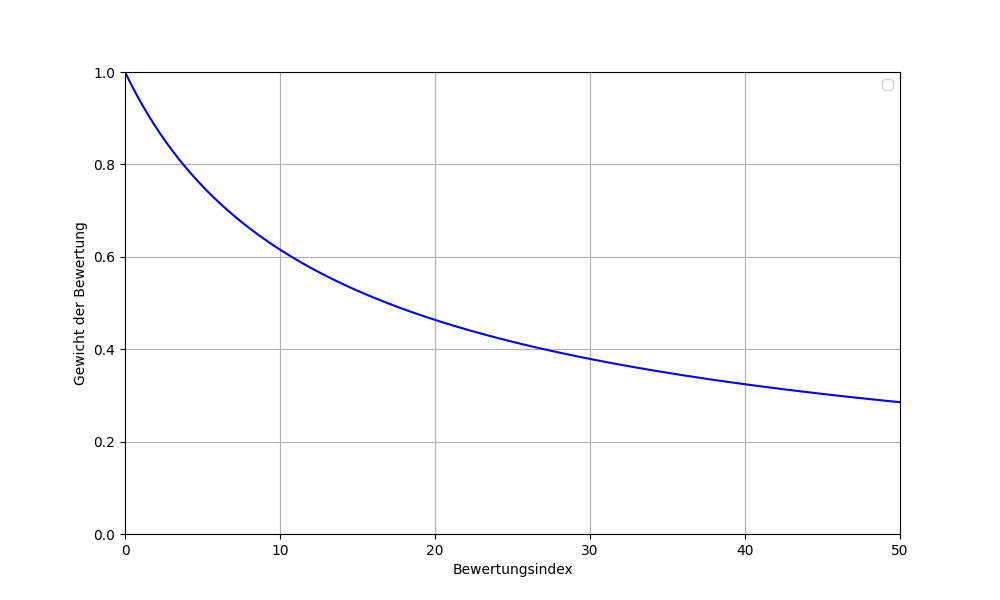
\includegraphics[width=0.8\linewidth]{ReputationWeights.png}
\end{figure}

Für die Neuberechnung werden (soweit vorhanden) die letzen 50 Bewertungen des DG nach Eingangszeitpunkt absteigend sortiert, sodass die neueste Bewertung an erster Stelle steht. Anschließend werden die Bewertungen mit einem Faktor multipliziert, der sich aus der Funktion $f(index)=(0,1\cdot index + 1)^{-0,7}$ ergibt. Der Graph der Funktion ist in Abbildung \ref{fig:reputationWeights} visualisiert. Danach werden alle vervielfachten Bewertungen aufsummiert und durch die Summe der Faktoren geteilt. Die Funktion bevorzugt die neuesten Bewertungen und verleiht ihnen größeren Einfluss auf den entgültigen Reputationswert. Dadurch kann sich ein Nutzer, der in der Vergangenheit viele gute Bewertungen erhalten hat, nicht in Sicherheit wiegen, sondern wird dazu angereizt konstant weiter gute Bewertungen zu erhalten.


%==================================================================================================


\chapter{Evaluation}
\label{chap:auswertung}
Nun da die Formalisierung des Konzepts abgeschlossen ist, kann mit der Auswertung begonnen werden. Dafür wird das Konzept hauptsächlich bezüglich der Sicherheit und des Rechenaufwands analysiert. Für die Analyse der Sicherheit werden die Angreifermodelle aus Kapitel \ref{chap:req} aufgegriffen und weiter spezifiert. Anhand von ihnen wird gezeigt, welche Schwachstellen das Konzept gegen die verschiedenen Angreifer aufweist. Zur Analyse des Rechenaufwands werden gemessene Laufzeiten der Implementation begründet und miteinander verglichen. Später wird zusätzlich geprüft, ob die in Kapitel \ref{chap:req} gesetzten Anforderungen erfüllt wurden, sowie Antworten auf die in Kapitel \ref{chap:intro} genannten Foschungsfragen besprochen. Zum Schluss gibt es eine Diskussion mit bestehenden Problemen und weiterführenden Ansätzen.
\section{Bewertung der Sicherheit}
\label{sec:auswertungSecurity}
Die Sicherheit eines Systems in Bezug auf verschiedene Angriffe, ist ein essenzieller Faktor für den Erfolg dieses Systems. Insbesondere bei kryptographischen Protokollen, wie Keyexchange Protokollen oder dem in Kapitel \ref{chap:systems} präsentierten Bezahlsystem, ist die Sicherheit einer der entscheidenen Punkte. Um einen Standard für eine Bewertung der Sicherheit einzuführen, definierten D. Dolev und A. Yao im Jahr 1983 das erste Angreifermodell \cite{am-dolev1983security}. Ein Angreifermodell beschreibt einen theoretischen Angreifer, der probiert, dem zu untersuchenden System Schaden zuzufügen oder Informationen zu extrahieren. Dafür müssen die Rahmenbedingungen des Angreifermodells genau bestimmt werden. Es umfasst in der Regel Angreiferziele, Angreiferannahmen und Angreiferfähigkeiten \cite{am-do2019role}. 
\begin{itemize}
    \item \textbf{Angreiferziele.} Für einen Angreifer gibt es mehrere Ziele, die er mit seinen Angriffen erreichen möchte. Er kann beispielsweise Interesse daran haben, die übertragenen Informationen mitzuschneiden, Geheimnisse wie private oder Sitzungsschlüssel herauszufinden oder die Kommunikation vollständig zu verhindern. 
    \item \textbf{Angreiferannahmen.} Sie beschreiben das Umfeld und die Ressourcen des Angreifers. Häufig auftretende Annahmen sind die Unterscheidung zwischen externem oder internem Zugriff auf ein Netzwerk die Beschränkung auf einen polynomial probabilistischen Angreifer, was beschreibt dass der Angreifer nur $O(n^k)$ Rechenaufwand bei einer Konstanten $k$ und Eingabelänge $n$ hat und bei der Berechnung zufällige Werte raten darf.
    \item \textbf{Angreiferfähigkeiten.} Die Fähigkeiten eines Angreifers sind durch seine Handlungsmöglichkeiten definiert. So kann ein aktiver Angreifer die Fähigkeiten besitzen, Botnetzwerke zu verwenden um DDoS Attacken zu starten, per Brute Force zu probieren ein Passwort zu knacken oder Analysen des Geheimtexts durchzuführen, die Schlüsse auf die übertragene Nachricht oder verwendeten Schlüssel zulassen. Passive Angreifer hingegen haben meist nur die Möglichkeit, die Kommunikation zu beobachten und Schlüsse aus dem Netzwerkverkehr abzuleiten.
\end{itemize} 
Zusammen ergibt die Definition des Angreifermodells eine maximale Stärke die ein Angreifer besitzen und trotzdessen das System nicht brechen kann. Sollte er in nur wenigen Punkten mehr Macht besitzen als das Angreifermodell vorgibt, so ist die Sicherheit des Systems nicht mehr gewährleistet und der Angreifer kann sein definiertes Ziel erreichen. Daher spricht die Aufstellung eines starken Angreifermodells und die Verteidigung gegen dieses für die Robustheit des Systems. Eine genaue Definition des Angreifermodells ist wichtig, da unpräzise Formulierungen ein mehrdeutiges Angreifermodell liefern, das nicht genau bestimmen kann, wogegen das System geschützt ist.

\subsection{Angreifermodelle der Coin Generierungsphase}
\label{subsec:adversaryCoinGen}
Bei einer Durchführung des Coin Generierungsprotokolls treten Exchange (EX) und Datennutzende (DN) als Akteure auf. Für jeden von ihnen muss ein Angreifermodell definiert werden, um die Sicherheit bei korrumpierten Kommunikationsteilnehmern zu zeigen. Zusätzlich soll die Sicheheit gegen einen außenstehenden Angreifer gezeigt werden.

\paragraph{Bösartiger DN.}
Ein bösartiges Verhalten eines DN kann durch eine Übernahme eines DN durch einen externen Angreifer oder durch bösartige Interessen des DN selbst entstehen. In beiden Fällen ist das Ziel des Angreifenden, entweder Coins mit größerem monetären Wert zu erhalten als der ursprüngliche Zahlungseingang beim EX zulässt oder eine Möglichkeit zu erhalten, selbst Coins zu signieren. Die dafür zu treffenden Annahmen sind, dass es sich um einen aktiven Angreifer handelt. Er verfügt über unbegrenzten Speicher und kann Algorithmen mit polynomieller probabilistischer Rechenzeit ausführen. Zusätzlich kennt er den PK des EX und den für den Zahlungseingang verwendeten $AccountPublicKey$ $(APK)$. Mögliche Angriffe die er starten kann, sind Replay-Attacken, welche eine zuvor gesendete Nachricht wiederholen, sowie Chosen-Plaintext-Attack, bei denen der Angreifer den Nachrichteninhalt bestimmt und observieren kann wie sich der Geheimtext verhält, sowie Brute-Force-Attacken zum Erraten des SKs und Geheimtextanalysen zur Herausarbeitung des SKs.\\

Da der Ablauf des Zahlungseingangs in Schritt 1 hauptsächlich von der konkret verwendeten Methode abhängt, kann hier davon ausgegangen werden, dass der Angreifer eine reguläre Transaktion leistet, da er ohne den damit entstehenden $CoinGenerationToken$ das Protokoll nicht fortführen kann. 
Anschließend erfragt er beim EX alle Token mit dem verwendeten $APK$. Nach Erhalt des soeben erstellten Token, kann er probieren Coins zu generieren, die den $ES$ Wert des Token übersteigen und den $value$ zusammen mit dem Token zum EX zu senden. Da der EX zuerst den summierten $value$ Betrag aller Coins mit dem $ES$ des Tokens vergleicht, wird der EX bereits hier feststellen, dass ein Angreifer probiert, mehr Geld zu erhalten, als er bezahlt hat. Der Versuch schlägt hier fehl.

Der Angreifer ist daher gezwungen, eine zum $ES$ passende Menge an $values$ zu generieren und zu übertragen. Der EX antwortet mit einer Liste von $a,b$ für jeden $value$. Nun kann der Angreifer sich entscheiden, das Protokoll für partiell blinde Signaturen (Abschnitt \ref{sec:partBlindSig}) zu verlassen und anstatt die vorgesehene Berechnung für $e$ auszuführen, $e$ als Variable für den Chose-Plaintext-Angriff zu verwenden. Er schreibt jedem $e$ einen leicht veränderten Wert zu, sendet diesen an den EX. Er erhält für jedes $e$ ein Tupel aus $(r,c,s,d)$ und kann probieren, die Unterschiede zwischen den verschiedenen $r$ mithilfe der Geheimtextanalyse herauszuarbeiten. Da der EX zur Berechnung von $r$ zwei dem Angreifer unbekannte Variablen benutzt ($u,x$) und auf das Ergebnis $mod$ $q$ anwendet, ist bei einer ausreichend großen Wahl von $u,x,q$ anzunehmen, dass das Ergebnis pseudozufällig erscheint und keine Hinweise auf $x$ liefert. Dabei verliert der Angreifer zusätzlich bei jedem Versuch den Wert des Coins, da die entstehende Signatur nicht gültig ist.

Sollte der Angreifer $e$, wie vom Protokoll vorgesehen, berechnen und nach Erhalt von $(r,c,s,d)$ probieren $u,x$ zu erraten, sodass die Ergebnisse seiner Berechnung mit $(r,c,s,d)$ übereinstimmen, kann er diesen Brute-Force-Angriff ohne Verlust von Coins starten. Solange $q$ groß genug gewählt ist (in der Implementierung 128bits) mit $u{\in}_{R} {\mathbb{Z}}_{q}$ ist die Chance allein $u$ korrekt zu bestimmen bereits $\frac{1}{2^{128}} \approx \frac{1}{3,4\cdot10^{38}}$ ausreichend gering, um das Gelingen des Erratens von $u$ und $x$ als vernachlässigbar anzunehmen.

Der Angreifer kann auch probieren, anhand des PKs des EX einen Faktorisierungsalgorithmus laufen zu lassen, um den SK zu bestimmen. Noch sind aber keine Algorithmen bekannt, die das Faktorisierungsproblem in aufbringbarer Zeit effizient lösen können, weshalb der Angreifer auch mit diesem Vorgehen nicht an den SK kommt \cite{montgomery1994survey}.

Nach Ausstellung der Signatur ist der Wert jedes Coins fest zugeteilt. Wenn ein Angreifer versucht den $value$ des signierten Coins zu ändern, werden damit die Grundlagen zum Überprüfen der Signatur umdefiniert, was dazu führt, dass jede Validierung fehlschlägt. Somit verliert der Coin schlagartig seinen Wert, sobald der Angreifer den $value$ verändert.

Letztlich kann der Angreifer probieren, einen Replay-Angriff zu starten und einen bereits einmal eingesetzten $CoinGenerationToken$ erneut mit einer Reihe an $values$ zum EX zu senden. Jedoch ist in Kapitel \ref{system:coingeneration} definiert, dass der EX jeden erhaltenen $CoinGenerationToken$ auf eine doppelte Einlösung überprüft. Daher wird der EX die Annahme des Tokens verweigern und der Angreifer schafft es auch hier nicht, mehr Coins zu erhalten als ihm zustehen.

\paragraph{Neugieriger EX.}
Der EX stellt in der Coin Generierungsphase eine Rolle mit großer Verantwortung da. Er hat die Aufgabe, Geldsummen sicher zu verwalten und trotz der Anonymität des Konzeptes genau die passenden Mengen ein- und auszuzahlen. Trotzdem wird das Angreifermodell für den EX hier nur schwach definiert. Dies hat vor allem den Hintergrund, dass das Konzept eines EX zum Tausch von Geld in die jeweilige Kryptowährung bereits etabliert ist und viele Sicherheitsmaßnahmen bestehen, die den EX zu einem gutmütigen Verhalten zwingen \cite{gnu-burdges2016enabling,kim2018risk,baum2021p2dex}. Deswegen wird im Folgenden nur die Sicherheit des Protokolls gezeigt, aber nicht die Sicherheit des EX.
Angenommen der EX kann nicht durch Unbefugte übernommen werden, so sind seine Angreiferziele in Erfahrung zu bringen, welcher DN wie viele Coins besitzt und wie viel diese wert sind. Zusätzlich ist er daran interessiert herauszufinden, mit wem der DN -- der sich die Coins signieren lässt -- handelt. Dafür möchte er sowohl die Identität des DN als auch des Coins wiedererkennen und verschiedene Signiervorgänge untereinander verlinken können. Die Angreiferannahmen beschränken sich zum größten Teil auf passives Verhalten. Er hält sich überwiegend an das Protokoll und beobachtet die Kommunikation mit dem DN, um daraus Informationen zu sammeln. Seine Rechenleistung ist polynomial probabilistisch und er kennt sämtliche Informationen, die im ersten Schritt angegeben werden. Die Angreiferfähigkeiten sind ebenso eingeschränkt. In den meisten Fällen antwortet er auf Anfragen des DN, wie das Protokoll es vorgibt. Nur die Wahl der Berechnungswerte für die partiell blinde Signatur kann er variieren.\\

Wie bereits definiert, hält sich der EX zunächst an das Protokoll. Er erstellt beim Eintreffen einer Zahlung einen $CoinGenerationToken$ mit dem $APK$ und $ES$ gleich den Werten der Zahlung und legt diesen mit dem $APK$ verschlüsselt in seinem Speicher ab. Da der $APK$ ein regulärer PK ist, kann der EX keine fundierten Kenntnisse aus einem $APK$ ziehen. Erst sobald der selbe $APK$ für eine spätere Zahlung erneut angegeben wird, kann davon ausgegangen werden, dass der Zahlungseingang von der gleichen Person stammt. Wenn ein DN aber für jede Zahlung einen neuen $APK$ generiert, kann der EX zwei verschiedene Zahlungen nicht zu der gleichen Person zurückführen.

Auf Anfrage gibt er den $CoinGenerationToken$ heraus. Bei dem Berechnen der partiell blinden Signatur ist der einzige Wert, für den eine Abweichung vom Protokoll sinnvoll sein kann, der SK. Die Werte $u,s,d,z,c,r$ sind bei jedem signierten Coin unterschiedlich. Diese gleich zu behalten würde ab dem zweiten Coin dem DN auffallen. Der SK hingegen ist dem DN nicht bekannt und die Auswirkung beim auswechseln des SKs sind nicht feststellbar. Daher kann der EX probieren, für jeden signierten Coin einen eigenen SK zu verwenden. Dadurch kann er beim späteren Erhalt von Coins im Bezahlsystem durch den DG nachvollziehen, aus welcher Signieranfrage der Coin stammt und kann so die Beziehung zwischen dem DN und DG vermuten. An dieser Stelle greift jedoch der $BDLEQ$, welcher in \ref{sec:privacy-pass} erklärt wurde und verhindert, dass der EX unbemerkt den SK austauschen kann. Bei einem Versuch den SK zu ersetzen, zeigt der $BDLEQ$, dass der verwendete SK nicht mehr mit dem beworbenen übereinstimmt. Somit ist der EX gezwungen den gleichen SK einzusetzen, was die potenzielle Wiedererkennung im späteren Verlauf verhindert.\\

Da für das Anfragen einer Signatur der Coin partiell geblendet wird, ist nur dessen $value$ für den EX sichtbar. Der $nonce$ der dem Coin seine Identität verleiht, bleibt vor dem EX vorerst versteckt. Daher hilft einem EX der bei einem Signiervorgang erhaltene $nonce$ nicht dabei, den selben Coin beim Einlösen wiederzuerkennen. In Kapitel \ref{system:coingeneration} wird zusätzlich vorrausgesetzt, dass der $value$ des Coins aus einer kleinen Menge an möglichen Werten ausgewählt sein muss. Wenn sich ein DN nicht an diese Vorschrift hält und einen Coin mit beispielsweise $123,45$\texteuro\ signieren lassen will, kann sich der EX diesen $value$ merken. Wenn dieser Betrag so einzigartig ist, dass ihn kein anderer DN ebenfalls benutzt hat, so kann der EX beim Einlösen eines Coins mit dem $value = 123,45$\texteuro\ sicher sein, dass der DG diesen Coin im Handel mit dem DN erhalten hat, dessen $APK$ er sich gemerkt hat. Solange jedoch jeder DN die $values$ seiner Coins aus der Mengen an möglichen Werten auswählt, gibt es für jeden $value$ eine große Anzahl an Vorkommnissen, die es dem EX unmöglich macht mit Sicherheit einen eingelösten Coin zu einer Signieranfrage zu verlinken.

Daher bleibt dem EX keine Möglichkeit die Identität eines DN über mehrere Signieranfragen zu verlinken, solange er für jede Anfrage einen neuen $APK$ verwendet. Des Weiteren muss der EX die Coins mit dem gleichen SK signieren, was eine Verlinkung über verschiedene SKs ausschließt und kann anhand des $values$ keine Zusammenhänge zwischen Signier- und Einlösephase treffen. Zusammen bedeuted dies, dass er seine Angreiferziele nicht erreicht.

\paragraph{Außenstehender Angreifer.} Der außenstehende Angreifer wurde bereits in dem Kapitel \ref{chap:req} kurz dargelegt. Seine Ziele sind es -- bezogen auf die Coin Generierungsphase -- selbst die Coins zu erhalten, für die der DN gezahlt hat. Zusätzlich möchte er den DN davon abhalten, seine Coins zu erhalten und die Möglichekeit besitzen, einen DN anhand von zwei Signieranfragen wiederzuerkennen. Die Annahmen über den außenstehenden Angreifer sind die Folgenden: Er ist ein externer Angreifer und daher kein vorgesehener Teilnehmer der Kommunikation. Er kennt den in Schritt 1 verwendeten $APK$ des DN, hat aber kein Wissen über den dazu gehörigen SK. Zudem hat er unbegrenzten Speicherplatz und verfügt über Algorithmen mit polynomieller Laufzeit. Seine Fähigkeiten umfassen das Ausführen von Brute Force Angriffen, Geheimtextanalysen und Replayangriffen. Außerdem kann er sämtliche Nachrichten, die während der Protokollausführung gesendet werden, mitschneiden und selbst die Kommunikation zum EX aufnehmen. Ein Man in the Middle Angriff ist jedoch nicht möglich.\\

Angenommen der Angreifer hat die erste Nachricht mit dem Eingang der Zahlung und dem $APK$ mitgeschnitten, so hat er die Informationen über sowohl die erhaltene Summe $ES$, als auch den $APK$. Da der in Schritt 2 übertragene $CoinGenerationToken$ mit dem $APK$ verschlüsselt ist, kann er die Nachricht nicht in realistischer Zeit entschlüsseln, da kein polynomieller Algorithmus bekannt ist, der ECC ohne Kenntnisse über den SK entschlüsseln kann \cite{ecc-bos2009security}. Es bleibt ihm die Möglichkeit, nachdem er die Nachricht mitgeschnitten hat, durch Brute Force zu versuchen den $nonce$ zu erraten, den daraus entstandenen Token mit dem $APK$ zu verschlüsseln und zu prüfen, ob das entstehenden Ergebnis sich mit dem mitgeschnittenen Token deckt. Allerdings ist einerseits der $nonce$ 128 Bit lang, was bedeutet, dass er $2^{128}$ Möglichkeiten durchprobieren muss, um den richtigen Wert zu finden. Andererseits er hat dafür nur solange Zeit, wie der DN zum Erstellen der Coins braucht, da der Token nach abgeschlossener Signtatur der Coins als benutzt gespeichert wird. Der Angreifer kann probieren, nach dem Mitschneiden der ersten Nachricht für alle möglichen $nonce$ den entsprechenden Token zu verschlüsseln und in einer Hashmap mit Zugriffszeit $O(1)$ abzulegen. Sollte es ihm gelingen alle $2^{128}$ möglichen Token zu Erstellen und Verschlüsseln, bevor der DN seinen $CoinGenerationToken$ beim EX anfragt, so kann ein Rennen zwischen Angreifer und DN entstehen, in dem der gewinnt, der zuerst seine Coins mit dem Token zum EX sendet. Solange aber von einer ähnlichen Berechnungszeit wie in \cite{nofriansyah2018efficiency} ausgegangen wird, braucht der Angreifer $0,02 \cdot 2^{128}\approx 6,8\cdot10^{36}$ Sekunden oder $2,16\cdot10^{29}$ Jahre, um diese vollständige Hashmap an Token anzulegen. Daher kann davon ausgegangen werden, dass der Angreifer nicht an den lesbaren $CoinGenerationToken$ kommt, bevor der DN diesen Verwendet.\\

Die anschließenden Schritte, welche die für die partiell blinden Signaturen nötigen Daten austauschen, sind ebenfalls alle mit dem $APK$, beziehungsweise mit dem PK des EX verschlüsselt, weshalb der Angreifer den passenden SK bestimmen müsste, um den Verkehr mitzulesen. Da es auch hier keinen Algorithmus gibt der dies in polynomieller Zeit schafft \cite{ecc-bos2009security}, kann angenommen werden, dass der Angreifer die Nachrichten nicht lesen kann. Somit erhält er keinen Zugang zu den vom DN generierten Coins. Auch die Identität des DN kann mitk einer anderen Signieranfrage verlinkt werden, solange der DN für jede Anfrage einen neuen $APK$ verwendet.

Um den DN vom Erhalt seiner Coins abzuhalten, fehlen dem Angreifer jegliche Fähigkeiten. Er kann zwar alle Nachrichten, die gesendet werden mitschneiden, aber die Übertragung nicht stören oder Nachrichten verschwinden lassen. Würden die Angreiferfähigkeiten auf das Verschwinden lassen von Nachrichten ausgeweitet werden, könnte er jede Nachricht des Protokolls wiederholt löschen und somit die Kommunikation vollständig verhindern. Der einzige Weg, auf dem er den DN sonst vom Erhalt seiner Coins abhalten kann, ist den $CoinGenerationToken$ vor ihm auszugeben, was wie zuvor erläutert unwahrscheinlich ist.

Angenommen er schafft es mit einer Geheimtextanalyse über die Unterschiede zwischen dem in Schritt 2 und in Schritt 4 übertragenen Token den Klartext des $CoinGenerationTokens$ zu bestimmen. Dann kann er probieren, eine Interaktion mit dem EX ab Schritt 4 zu starten und den Klartext des Tokens mit in die Anfrage zu senden. Dieser Versuch wird jedoch fehlschlagen, da der analysierte Token bereits beim EX eingelöst wurde und dieser ihn als $spent\leftarrow true$ gespeichert hat, was weitere Verwendungen des Tokens unterbindet. Der außenstehende Angreifer erreicht daher keines seiner Ziele.

\subsection{Angreifermodelle der Bezahlphase}
\label{subsec:adversaryPayment}
In der Bezahlphase des Systems steigt die Anzahl der Beteiligten im Vergleich zur Coin Generierungsphase um das Doppelte. Somit müssen für die Bewertung der Sicherheit des Bezahlsystems vier Angreifermodelle für die Beteiligten und ein zusätzliches für außenstehende Angreifer erstellt werden. Daraus ergeben sich insgesamt fünf Angreifermodelle gegen die die Sicherheit des Systems im Folgenden geprüft wird.

Vorab kann hier zusammengefasst werden, dass alle Angreifermodelle über unbegrenzten Speicherplatz verfügen und für das Ausführen jeglicher Angriffe nur Zugriff auf Algorithmen mit polynomieller Laufzeit haben.


\paragraph{Neugierig aber ehrlicher Datentreuhänder (DT).}
Kapitel \ref{chap:basics} beschreibt, dass die Rolle des DTs in der Verwaltung sowie Verbreitung der mit ihm geteilten Daten eine essentielle Rolle spielt.  Er ist dazu verpflichtet, im Sinne des DG zu handeln, weshalb hier nur von einem passiven Angreifer ausgegangen wird. Seine Ziele sind es, anhand der über ihn kommunizierten Daten herauszufinden, wie viel ein bestimmter DG handelt und mit welchem DN er Dienstleistung Handel eingeht. Der neugierig aber ehrliche DT ist ein passiver Angreifer, weshalb er an die genaue Ausführung des Protokollablaufs gebunden ist. Er darf diese nicht verlassen, sondern kann nur über ihn übertragenene Daten mitschneiden. Seine Angreiferfähigkeiten umfassen die Informationsgewinnung aus erhaltenen Nachrichten und mögliche Geheimtextanalysen dieser. Zusätzlich kann der neugierige DT mit bösaritgen DN zusammenarbeiten und zu einem beliebigen Zeitpunkt nachfragen, welche Informationen der DN bis zu diesem Zeitpunkt erhalten hat.\\

Das Erstellen eines Aufrufs in Schritt 1 des Bezahlsystemprotokolls in Kapitel \ref{system:payment} ist für das Erreichen der Angreiferziele uninteressant, da hier nur Informationen über den DN bekannt werden. Da sich die Ziele jedoch nur auf Informationsgewinnung über den DG beziehen, kann dieser Schritt unbeachtet bleiben. 

In Schritt 2 hingegen baut der DG das erste Mal eine Verbindung auf. Er überträgt jedoch keine Daten an den DT. Der DT weiß nach Antwort mit der Aufrufliste nur, dass der DG eine aktuelle Version der Liste besitzt. Diese Information hilft ihm allerdings nicht, da der folgende Schritt 4 über einen Proxy mit TLS gesendet wird. So kann der DT zwar die Integrität der Nachricht sicherstellen, kann aber nicht herausfinden wer die Nachricht gesendet hat. Die erhaltenen Daten umfassen keine Informationen, die auf die Identität des DG schließen lassen. Daher bringt selbst -- nachdem der DN in Schritt 6 die Daten erhalten und entschlüsselt hat -- eine Nachfrage des Klartextes der verschlüsselten Nachricht den DT nicht näher an sein Ziel. Dies gilt allerdings nur, solange wie in Abschnitt \ref{sec:systemAssumptions} angenommen wurde, dass der DT selbst nicht bestimmen kann, von welchem DG die an der $DataLocation$ angelegten Daten stammen.

Schritt 9 legt nur die $DataLocation$ offen, welche der neugierig DT nach einer Anfrage des Klartexts bereits weiß. Er lernt daher auch durch Schritte 9 und 10 keine wichtigen neuen Informationen über den DG. In Schritt 11 überträgt der DN die Coins für die Bezahlung zusammen mit dem $ReferenceCode$ an den DT. Der $ReferenceCode$ ist eine, für jeden Datenpostfacheintrag neu generierte Zahl, die keine Informationen des DG beinhaltet. Die Coins stammen vom DN, der diese selbst erstellt hat. Das Wissen über diese Nachrichteninhalte kann er beim DN erfragen. Es hilft ihm aber nicht dabei, Indizien über die Identität des DG zu finden.

Da der DG zum Abholen seiner verschlüsselten Coins aus dem Coinpostfach wieder einen Proxy mit TLS verwendet, weiß der DT nur, dass jemand die Coins zu dem $ReferenceCode$ abgefragt hat. Alle weiteren Daten über mögliche PKs des Anfragenden oder dessen $DG-ID$ bleiben geheim. Da die Coins mit $SHK$ verschlüsselt sind kann der DT davon ausgehen, dass die Coins von der gleichen Person abgefragt wurden, die den Datenpostfacheintrag in Schritt 4 gesendet hat. Er kann also den Eingang eines Datenpostfacheintrag und die Anfrage des Coinpostfachs verlinken. Jedoch kann er aus dieser Verlinkung keinerlei Wissen über den DG ziehen. Die Benutzung von TLS stellt sicher, dass der PK des DG nicht für die Anfragen der Postfächer verwendet wird, weshalb der DT auch hier nichts über den DG lernt. Da der DT keinen DG eindeutig bestimmen kann, kann er auch keine Aussage über die Handelsfrequenz eines DG treffen.

Die Anschließenden Schritte geschehen nur noch zwischen dem DG und dem EX, sodass weder der DT, noch der DN involviert sind. Somit erreicht der neugierig aber ehrliche DT sein Ziel, Informationen den DG und dessen Handelspartner zu gewinnen nicht, da er zu keinem Zeitpunkt weiß, welcher DG mit dem DN kommuniziert.

\paragraph{Bösartiger Datennutzender (DN).}
Wie bereits in Kapitel \ref{chap:req} erwähnt wurde, sind die Ziele eines bösartigen DN, herauszufinden, von welchem DG die erhaltenen Daten stammen. Des Weiteren liegt es in seinem Interesse, für den Erhalt von Daten keine Coins ausgeben zu müssen. Das dritte seiner Ziele ist es, den DG mit Hilfe des Streitfallsystems unrechtmäßig durch den DT bestrafen zu lassen. Dazu sei gesagt, dass in den meisten Streitfällen bei bewiesener Unschuld des DN, ein Ausbleiben der Zahlung die Konsequnz ist und daher die letzen beiden Ziele Hand in Hand gehen. Bei dem bösaritgen DN handelt es sich um einen internen Angreifer, der in die direkte Kommunikation mit dem DT verwickelt ist. Die erste Angreiferfähigkeit des bösaritgen DN besteht in der Kooperation mit einem neugierig aber ehrlichen DT, wie bereits im letzten Absatz aufgeführt. Er kann zu jedem Zeitpunkt von dem vorgegebenen Protokoll abweichen und beliebige Nachrichten senden.

Zuerst beginnt der DN in Protokollschritt 1 damit einen Aufruf zu Erstellen. Hier kann er bereits probieren, den ersten Streitfall aufzusetzen. Dafür gibt er dem Aufruf einen beliebigen $Call$-$PK$, dessen zugehöriger SK ihm nicht bekannt ist und sendet diesen Aufruf zum DT. Nachdem der DG den Aufruf angefragt und einen entsprechenden Datenpostfacheintrag gesendet hat, kann der DN diesen beim DT anfragen. Da er einen PK angegeben hat, über dessen Gegenstück er nicht verfügt, kann er den $SHK$ nicht entschlüsseln. Er meldet deswegen einen \textit{Fehlerhafte Verschlüsselung} Streitfall. Wie dort beschrieben ist, wird nach Ablauf des maximalen Bezahlzeitraums eine Beschwerde des DG eingehen, der nach dem Verbleib seiner Coins fragt. Dieser wird dazu aufgefordert, den $SHK$ mit dem DT zu kommunizieren. Nachdem der DT den $SHK$ mit dem angegebenen PK des Aufrufs verschlüsselt hat und sich die Ergebnisse mit dem Datenpostfacheintrag decken, fällt auf, dass der DN entweder den $SHK$ entschlüsseln kann oder einen falschen PK angegeben hat. In beiden Fällen wird hier der DN bestraft. Auch aus der Zusammenarbeit mit dem neugierigen DT lernt er nichts über den DG, solange dieser für die Klärung des Streitfalls weiterhin einen Proxy sowie TLS verwendet.

Angenommen der DN hätte in Schritt 1 einen gültigen $Call$-$PK$ angegeben, zu dem er einen SK besitzt, dann kann er in Schritt 9 die Daten der $DataLocation$ abfragen und diese nach dem Erhalt in Schritt 10 entschlüsseln. Meldet er nun den Streitfall \textit{Fehlerhafte Datenparameter}, so muss der DN den $SHK$ zum DT senden, welcher damit den Datenpostfacheintrag entschlüsselt, die $DataLocation$ abfragt und die dort liegenden Daten mit dem $DataKey$ entschlüsselt. Da der DG sich hier gutartig verhält, wird der DT feststellen, dass der DN die Daten lesen konnte. Somit wird wieder der DN bestraft aber nicht der DG. Beim Bewerten des Steitfalls lernt der DT die gleichen Informationen wie der DN, weshalb aus der Zusammenarbeit mit ihm keine neuen Informationen über den DG zum Voschein kommen.

Versucht der DN trotz qualitativ hochweritger Daten den Streitfall \textit{Nutzlose Daten} auszulösen, so wird die Überprüfung genauso abgehandelt wie im letzten Absatz. Dabei stellt sich wieder heraus, dass der DN betrügen wollte. Es werden keine Details bezüglich des DG preisgegeben.

Der nächste Ansatzpunkt ist in Schritt 11. Hier kann der DN zuerst probieren keine Coins zu übertragen. Da die gesamte Nachricht, in der sich die Coins befinden verschlüsselt ist, sieht der DT nicht, ob Coins enthalten sind. Erst nach Schritt 14, in dem der DG die Nachricht entschlüsselt hat, kann er den Streitfall \textit{Fehlerhafte Coins} auslösen und den $SHK$ sowie den $ReferenceCode$ zum DT senden. Nun kann dieser die Nachricht entschlüsseln. Da er keine Coins vorfindet, wird der DN bestraft. Das gleiche Verhalten kann in dem Fall angewendet werden, dass der DN zu wenig Coins überträgt. Wenn der DG zusätzlich einen Verweis auf den Datenpostfacheintrag mitsendet, so kann der DT den Aufruf bestimmen und den Preis dessen mit dem Wert der erhaltenen Coins abgleichen. Um für Daten nicht zu bezahlen kann der DN ebenfalls versuchen, selbst einen Coin zu erstellen und diesen zu übertragen. Nachdem der DG die Nachricht mit dem selbst erstellten Coin entschlüsselt hat, schlägt das Prüfen der Signatur fehl, woraufhin er den gleichen Streitfall auslöst und die gleiche Schlichtung geschieht. Als dritte Möglichkeit kann ein DN probieren, den gleichen Coin an mehrere DG zu bezahlen. Dieses Verhalten wird erst nach Schritt 16 erkannt. Beim Einlösen des Coins bei einem EX fällt auf, dass der Coin bereits vorher von einem anderen DG ausgegeben wurde. Deswegen stellt der EX -- wie in Schritt 16 beschrieben -- eine signierte Antwortnachricht aus, die belegt, dass der Coin von einem DN doppelt ausgegeben wurde. Nun kann der DG mit dieser Nachricht, dem $SHK$ und dem $ReferenceCode$ zum DT gehen, welcher nach einer Analyse des Beweismaterials wieder den DN bestraft. Dem DN bleibt also nichts anderes übrig, außer dem DG eine korrekte Menge an signierten Coins zu bezahlen, die noch nicht ausgegeben wurden.\\

Zum lösen der Streifälle wird wieder nur der $SHK$, der $ReferenceCode$ und gegebenenfalls die Nachricht des EX benötigt. Die ersten beiden, sind wie zuvor dargestellt wurde, zufällig. Die Nachricht des EX gibt keine Informationen über den DG. Da der EX die signierte $DG-ID$ beim Einlösen erhält, kann er mit Sicherheit sagen, dass die Coins von einem anderen DG eingelöst wurden. Welcher andere DG dies ist, behält er für sich. Nach Schritt 12 sind alle Interaktionen des DN innerhalb des Protokolls abgeschlossen. Er hat es weder geschafft Informationen über den DG herauszufinden, noch den DG unrechtmäßig zu bestrafen und wurde dazu gezwungen, die korrekte Menge an Coins zu bezahlen. Er hat also keines seiner Ziele erreicht.

\paragraph{Bösartiger Datengebender (DG).}
Das Angreifermodell eines bösartigen DG wurden bereits in Kapitel \ref{chap:req} kurz genannt. Ein bösartiger DG verfolgt eine Liste an Angreiferzielen. Das erste Ziel ist, ohne Daten an Coins des DN zu gelangen. Er will in der Lage sein, Coins von anderen DG zu stehlen und selbst einzulösen. Zusätzlich möchte er den DN durch das Streitfallsystem unrechtmäßig bestrafen lassen. Bei einem bösartigen DG handelt es sich um einen aktiven Angreifer, der Nachrichten sendet und von dem definierten Protokoll nach belieben abweichen kann. Er ist intern in die Kommunikation eingebunden, da er direkt mit dem DT und dem EX kommuniziert. Die Angreiferfähigkeiten eines bösaritgen DG sind das Ausführen von Brute Force Angriffen und das Erstellen einer Geheimtextanalyse.

Zu Beginn in Protokollschritt 2 fragt der DG nach der aktuellen Aufruflist. Der DT antwortet mit der Liste aus denen sich der DG einen aussucht. Da er dem DN keine Daten zur Verfügung stellen möchte, kann er nun entweder eine fälschliche $DataLocation$ angeben, die auf leeren Speicherplatz beim DT zeigt oder einen fälschlichen $DataKey$, der die Daten der $DataLocation$ nicht entschlüsseln kann. Natürlich kann er auch beides gleichzeitig verwenden. Die inkorrekten Datenparameter verschlüsselt er nun mit dem neu generierten $SHK$ und sendet sie an das Datenpostfach des Treuhänders. Da der DN die Daten nach dem Anfragen und entschlüsseln nicht lesen kann, wird er keine Bezahlung ausstellen, sondern den Streitfall \textit{Fehlerhafte Datenparameter} auslösen. Wie die Schlichtung des Streitfalls vorsieht, prüft der DT die Inkorrekheit der Datenparameter und wartet auf eine Rückmeldung des DG. Da der DG an dem Erhalt der Coins interessiert ist, wird dieser sich nach Ablauf des Bezahlzeitraums beim DT melden und nach dem Verbleib seiner Bezahlung fragen. Da der Steitfall für den DN entschieden wurde, erhält der DG keine Bezahlung. Ein ähnlicher Ablauf findet statt, wenn ein DG absichtlich qualitativ schlechte Daten hochlädt. Hier löst der DN den Streitfal \textit{Nutzlose Daten} aus. Der einzige Unterschied in der Behandlung besteht darin, dass der DT mit einem Qualitätssicherungsmechanismus die Daten als ungenügend bewertet. Das entstehende Ergebnis ändert sich jedoch nicht.

Ein bösartiger DG kann versuchen, einen Coinpostfacheintrag, der für einen anderen DG bestimmt ist, zu entschlüsseln und dessen Coins selbst einzulösen. Alle Coinpostfacheinträge sind durch jeden Anfragbar. Daher kann ein bösartiger DG zufällige Zahlen als $ReferenceCode$ durch probieren und wird je nach Handelsfrequenz des DT nach einer bestimmten Zeit einen Coinpostfacheintrag zurückerhalten. Angenommen der Postfacheintrag ist neu und wurde noch nicht -- von dem DG, zu dem dieser Eintrag gehört -- eingelöst. Dann könnte ein bösartiger DG die Coins dieses Eintrags selbst einlösen. Dafür muss er jedoch an den Klartext der Nachricht gelangen. Da die Coins mit einem 128 Bit AES Schlüssel verschlüsselt sind, muss er einen Weg finden diesen Schlüssel zu bestimmen. Aktuell ist keine effiziente Methode bekannt, um von einem AES-128 Geheimtext zum Schlüssel zu gelangen \cite{aes-Biryukov2010Key}. Deswegen kann der DG einen Brute Force Angriff starten, um den Schlüssel zu bestimmen. Das Entschlüsseln einer AES Nachricht dauert mit einem 128 Bit langen Schlüssel etwa 85 Millisekunden \cite{aes-Kumar2016Implementation}. Um also alle $2^{128}$ Schlüssel durchzuprobieren, wären $85\cdot 2^{128} \approx 2,89\cdot10^{40}$ Millisekunden oder $9,17\cdot10^{29}$ Jahre nötig. Das Knacken der Verschlüsselung ist also in einsehbarer Zeit unwahrscheinlich. Der einzige andere Weg an den Schlüssel zu gelangen ist, diesen aus der Verschlüsselung des Datenpostfacheintrages zu erschließen. Das Knacken dieser Verschlüsselung des Datenpostfacheintrags dauert -- wie oben gezeigt -- jedoch ähnlich lange. Es kann also davon ausgegangen werden, dass der DG an keinen Coin herankommt, der nicht für ihn bestimmt ist. 

Die einzigen beiden Streitfälle, die durch den DG ausgelöst werden können, sind \textit{Fehlerhafte Coins} und \textit{Überschreitung des Bezahlzeitraums}. Um also den DN unrechtmäßig zu bestrafen müsste ein bösartiger DG es schaffen, in einem der beiden Fälle den DT zu täuschen. Beim Überprüfen des Bezahlzeitraumes ist dies schwer. Durch das offenlegen des $SHK$ und des Datenpostfacheintrags, kann der DT den in dem Eintrag gespeicherten $ReferenceCode$ auslesen und entscheiden, ob ein Coinpostfacheintrag mit diesem $ReferenceCode$ existiert. Da der Datenpostfacheintrag beim Treuhänder gespeichert ist, kann er nicht verändert werden. Solange der $SHK$ und der Datenpostfacheintrag zusammenpassen, sind die Informationen für DN und DT eindeutig und unveränderlich, weshalb eine Täuschung hier schwer ist. Beim \textit{Fehlerhafte Coins} Streitfall kann -- wenn dieser nach Schritt 14 eintritt -- auch leicht durch den DT die Signatur überprüft werden. Tritt der Streitfall nach Schritt 16 ein, so ist dieser nur gülitg, wenn der DG eine signierte Nachricht des EX vorzeigt. Also ist in diesen beiden Fällen ein Täuschung ausgeschlossen, solange der DG kein Wissen über den SK des EX besitzt. Der bösaritge DG erreicht also keines seiner Ziele durch die hier beschriebenen Wege.

\paragraph{Neugierig aber ehrlicher Exhchange (EX).}
Ein neugierig aber ehrlicher EX ist nur zu einem kleinen Teil an der Kommunikation beteiligt. Er kommuniziert nur mit dem DG beim Einlösen von dessen Coins. Die Angreiferziele eines neugierig aber ehrlichen EX sind es, eine Beziehung zwischen dem -- ihm bekannten -- DG und dem DN -- von dem die Coins stammen -- herzustellen. Der neugierig aber ehrliche EX ist ein passiver Angreifer, der der Kommunikation lauscht und sich strickt nach Vorgabe des Protokolls verhält. Seine einzige Angreiferfähigkeit besteht in dem Mitschneiden der erhaltenen Daten und dem Versuch aus ihnen Informationen bezüglich seiner Angreiferziele zu erlangen.

Da der EX nur in den Protokollschritten 15 und 16 angesprochen wird, ist sein Handlungsumfang deutlich eingeschränkt. In diesen Schritten erhält er Coins von einem DG, um diese gegen Echtgeld zu tauschen. Da durch die Funktionsweise vorgeben ist, dass ein DG seine signierte ID übermitteln muss, weiß ein EX zu jeder Zeit, welcher DG bereits wieviel ausgezahlt bekommen hat. Jedoch nennt ihm der DG die Herkunft der Coins nicht. Um diese zu bestimmen, kann der EX einen gegebenen Coin auf seine Werte untersuchen. Dabei ist der ausschlaggebende Wert der $nonce$ der Coins. Der $value$ des Coins ist durch die Wahl aus der Menge an möglichen Werten $MV$ weit verbreitet. Alle Werte zum Prüfen der partiell blinden Signatur sind dem EX neu, da sie nach der letzten Interaktion vom DN bei dem Erstellen berechnet werden \cite{abe2000provably}. Der $nonce$ selbst ist dem EX ebenfalls neu, da dieser in dem Protokoll der partiell blinden Signaturen nicht im Klartext übermittelt wird. Da der EX durch den BDLEQ dazu gezwungen wird, immer den selben SK zum Signieren zu verwenden, ist ein Informationsgewinn durch die Verwendung verschiedener Schlüssel ausgeschlossen. Somit kann der EX einen vom DG erhaltenen Coin nicht mit einem in der Coin Generierungsphase signierten Coin verlinken. Da der DG keine Informationen über den Ursprung des Coins liefert, kann der EX den DN nicht bestimmen, weshalb er sein Ziel nicht erreicht. 

\paragraph{Außenstehender Angreifer.}
Das Angreiferziel des außenstehenden Angreifers ist in dem Bezahlsystem, die kommunizierten Daten oder Coins mitzulesen. Zusätzlich möchte er herausfinden, welcher DG mit welchem DN handelt. Die Angreiferannahmen und -fähigkeiten decken sich mit denen des außenstehenden Angreifers der Coin Generierungsphase.

Sowohl die $DataLocation$, der $DataKey$, als auch die Coins sind mit AES-128 verschlüsselt. Damit der außenstehende Angreifer diese lesen kann, müsste er also die Verschlüsselung knacken, was -- wie oben bereits beschrieben -- etwa $10^{29}$ Jahre dauern würde und daher in realistischer Zeit nicht möglich ist. Der Kommunikationsweg zwischen DG und EX in den Schritten 15 und 16 ist mit ECC verschlüsselt, welches zum Knacken eine vergleichbare Zeit benötigt. Der Angreifer kann versuchen, bei der Übertragung eines Datenpostfacheintrags in Schritt 4, den $SHK$ durch einen ihm bekannten AES Schlüssel zu ersetzen, um so im späteren Verlauf Zugang zu den übertragenen Coins zu erhalten. Damit zusammen muss er auch den $ReferenceCode$, $DataLocation$ und $DataKey$ selbst verschlüsseln und beifügen. Da der Angreifer die Werte dieser aus der Originalnachricht nicht kennt, muss er eigene Datenparameter angeben oder welche verwenden, die er auf anderem Weg abgegriffen hat. Dieser Versuch wird durch TLS erkannt, da dieses die Nachricht mit Integrität schützt, weshalb die Veränderungen der Angreifer festgestellt werden. Der Zugang zu den Daten bleibt ihm bei dieser Methode ohnehin verwährt. 

Für eine Verlinkung zwischen DG und DN müsste der außenstehende Angreifer mehr Informationen über den DG in Erfahrung bringen als es der DT oder DN schaffen. Durch die Verwendung von Proxys und TLS zum Senden des Datenpostfacheintrags sowie zum Abfragen des Coinpostfachs, bleibt der DG jedoch vollständig anonym und kann auch durch das Mitschneiden sämtlicher kommunizierter Nachrichten nicht nachverfolgt werden. Der außenstehende Angreifer erreicht keines seiner Ziele.

\subsection{Angreifermodelle des Reputationssystems}
\label{subsec:adversaryRep}
Da das Bezahlsystem unabhängig von dem Reputationssystem eingesetzt werden kann, wurde die Sicherheit getrennt von dem Reputationssystem betrachtet. Im Folgenden wird die Sicherheit des Reputationssystems gezeigt, um das Gesamtsystem -- bestehend aus Bezahl- und Reputationssystem -- auf seine Sicherheit zu prüfen.

\paragraph{Neugierig aber ehrlicher DT.}
Das Angreifermodell des neugierig aber ehrlichen DTs muss im Vergleich zu Absatz \ref{subsec:adversaryPayment} etwas gelockert werden. Der DT darf nun nicht mehr mit einem DN zusammenarbeiten und Nachrichten austauschen. Zudem werden Informtionen, die bei Schlichtung eines Streitfalls bekannt werden nicht beachtet, da der DT selbst keinen Streitfall auslösen kann. Da die Schlichtung ein unregelmäßiges Vorkommnis ist, erfährt der DT nur stichprobenartig Informationen über den Handel zwischen DG und DN. 

Das Hinzufügen des Bewertungstoken in dem Reputationsprotokoll aus Kapitel \ref{system:reputation} liefert dem DT keine neuen Informationen. Aus seiner Sicht wird der empfangene verschlüsselte Text länger, aber er kann nicht erkennen, welcher Bewertungstoken in einer Nachricht enthalten ist. Nachdem der DN den Datenpostfacheintrag erhalten und entschlüsselt hat, sendet er die verschlüsselte $DG-ID$ per Proxy und TLS an den DT und fragt nach der Reputation des DG. Die Verwendung von TLS und Proxy macht es dem DT unmöglich, den fragenden DN zu bestimmen. Warum der DT anhand der Menge an Anfragen nicht auf die Handlungsfrequenz schließen kann wird, in Abschnitt \ref{sec:ratingObfuscation} erklärt. Nachdem der DN die Daten des Postfacheintrags erhalten und ausgewertet hat, kann er eine Bewertung der Daten ausstellen. Dafür sendet er den Bewertungstoken zusammen mit einer Bewertung und einem DN Zertifikat an den DT. Der DT kann den Token validieren und anhand der enthaltenen, verschlüsselten $DG-ID$ die Bewertung einem DG zuweisen. Da auch hier die Nachricht mit der Bewertung über Proxy und TLS versendet wird, kennt der DT den DN nicht. Der DT kann also weder bestimmen, von welchem DN die Bewertung stammt, noch herausfinden, ob die Bewertung mit einem Handel zusammenhängt oder ob sie der Verschleierung dient. Er erreicht keines seiner Ziele. 

\paragraph{Bösartiger DN.}
Bei dem Angreifermodell des bösartigen DN können beinah alle Punkte des bösartigen DN aus Abschnitt \ref{subsec:adversaryPayment} übernommen werden. Ihm wird ebenfalls die Zusammenarbeit mit dem DT untersagt. Seine Ziele erweitern sich um das Abgeben mehrerer Bewertungen für einen Handel. Er möchte weiterhin die Identität des DG bestimmen, den DG unrechtmäßig durch einen Streitfall bestrafen und für einen Handel keine Coins ausgeben.

In dem übertragenen Bewertungstoken ist die ID des DG gespeichert. Allerdings muss der DN, um diese lesen zu können, zuerst die Verschlüsselung der ID knacken oder das Wissen über den SK des DT erlangen. Die Sicherheit des 256 Bit langen ECC Schlüssels wurde bei der Behandlung der obigen Angreifermodelle bereits gezeigt. Mit einer erwarteten Zeit von ungefähr $2,16\cdot10^{29}$ Jahren kann davon ausgegangen werden, dass es dem Angreifer nicht gelingt die Verschlüsselung zu knacken. Das Erhalten des SKs des DTs ist ebenso unwahrscheinlich, da dieser unter keinen Umständen den SK herausgibt. Die $DG-ID$ bleibt für den bösartigen DN unleserlich. Da für die Verschlüsselung der ID ein Saltwert verwendet wurde, ist der Geheimtext der ID selbst bei wiederholtem Verschlüsseln jedes Mal unterschiedlich. Der DN weiß daher nicht, ob er erneut mit dem selben DG handelt.

Um das Ziel des Bezahlsystems weiterzuverfolgen -- keine Coins für einen Handel bezahlen zu müssen -- kann er versuchen, den \textit{Zu niedrige Reputation} Streitfall auszulösen. Dafür übergibt er dem DT den SHK. Dieser entschlüsselt den Datenpostfacheintrag und die in dem Bewertungstoken enthaltene DG ID. Anschließend kann der DT prüfen, ob der DG eine ausreichend hohe Reputation für den angegeben Aufruf besitzt. Da hier von einem gutartigen DG ausgegangen wird, reicht seine Reputation aus. Als Resultat wird der DN bestraft und muss weiterhin die Coins an den DG senden. Der Versuch, die anderen Streitfälle (Kein/Dopplter Bewertungstoken, Inkorrekte Signatur) auszulösen, scheitert ebenfalls nach der Bewertung des DTs. Da der DG einen neuen Bewertungstoken gesendet hat, ist dessen $nonce$ noch nicht verwendet worden. Sollte der DN versuchen die Signatur des DG zu ändern und damit invalide zu machen, so wird dieses Verhalten beim Entschlüsseln des Datenpostfacheintrags bemerkt.

Abschließend kann ein bösaritger DN versuchen einen, Bewertungstoken zwei Mal auszugeben und so zwei Bewertungen für einen Handel auszustellen. Dieser Versuch misslingt ebenfalls, da der DT den $nonce$ des Tokens bereits in seiner Datenbank vorfindet und daher die Bewertung ablehnt. Der bösartige DN kann keines seiner Ziele erreichen.

\paragraph{Bösartiger DG.}
Die Ziele eines bösartigen DG sind ähnlich wie in Abschnitt \ref{subsec:adversaryPayment}, den DN durch die Ausnutzung des Streitfallsystems zu unrecht bestrafen zu lassen. Ein bösaritger DG will verhindern, dass er bewertet wird oder möchte Einfluss auf die Bewertung nehmen. Außerdem möchte er einem DN finanziell durch das Veröffentlichen dessen Aufrufe schaden. Dazu gehört beispielsweise auch das Abgeben eigener Bewertungen. Die Angreiferannahmen sowie -fähigkeiten können aus Abschnitt \ref{subsec:adversaryPayment} übernommen werden.

Um das Ausstellen einer Bewertung durch den DN zu unterbinden, kann ein bösaritger DG den dafür nötigen Bewertungstoken aus dem Datenpostfacheintrag entfernen. Dem DN fällt jedoch direkt nach Entschlüsseln des Eintrags der fehlende Token auf. Er alarmiert den DT, liefert den Postfacheintrag und $SHK$ und lässt den DT das Fehlen des Tokens validieren. Kann dieser das Fehlen bestätigen, so ist der DN nicht mehr zum Bezahlen verpflichtet. Der gleiche Vorgang wird durchlaufen, falls der DN einen Bewertungstoken mit dem gleichen $nonce$ zum zweiten Mal erhalten sollte. Weiter kann ein DG versuchen den gleichen Token zwei unterschiedlichen DNs zu senden. Dadurch kann eine Doppelausgabe erst in Schritt 11 festgestellt werden, in dem der DT den Bewertungstoken empfängt. Findet der DT den erhaltenen Bewertungstoken $nonce$ bereits in seiner Datenbank, so weist er den DN daraufhin, dass der Token zuvor schon benutzt wurde und es sich um einen Betrug handelt. Das Unterbinden einer Bewertung kann ein bösartiger DG somit nicht unbemerkt verhindern, solange der DN eine Bewertung abgeben möchte. Entscheidet sich ein DN dazu, die Bewertung zu überspringen, so kann der Test auf doppelte $nonce$ beim DT nicht ausgeführt werden. Da der DN in dem Fall aber nicht an der Abgabe einer Bewertung interessiert ist, ist die Unterbindung hier irrelevant.

Damit ein bösartiger DG Einfluss auf eigene Bewertung erhält, muss er entweder selbst Bewertungen einreichen oder DN dazu verleiten, gute Bewertungen auszustellen. Das was einen DG davon abhält, Bewertungen über sich selber abzugeben, ist die Vorzeigepflicht des DN Zertifikats. Ausschließlich DN verfügen über solch ein Zertifikat, was bedeuted, dass ein bösaritger DG nicht in der Lage ist, Bewertungen über sich selbst beim DT einzureichen. Die Höhe der ausgestellten Bewertung wird allein durch den DN bestimmt. Der DG ist aufgrund der Verschlüsselung mit ECC nicht dazu in der Lage die Bewertung zu verändern. Der einzige Weg wie ein DG Einfluss auf die Bewertung nehmen kann, ist das Bereitstellen von guten Daten. Wenn die Daten eine gute Qualität haben, wird die Bewertung des DN besser ausfallen, womit das System genau das erreicht worauf es abzielt.

Es ist anzumerken, dass ein DG mit hoher Reputation die vollständige Aufrufliste veröffentlichten kann und so auch DG mit niedriger Reputation die Chance gibt, Daten für Aufrufe bereitszustellen, zu denen sie keinen Zugang haben sollten. Der dadurch entstehende Schaden ist jedoch gering, da ein DN bei Erhalt von Daten die Reputation des DG prüfen kann und im Zweifel den \textit{Zu niedrige Reputation} Streitfall ausrufen kann. Er erhält also entweder kostenlos Daten oder geht mehr legitime Handel ein. Nachteile können durch die Veröffentlichung nur entstehen, wenn viele völlig nutzlose Daten geteilt werden, die einen erhöhten Rechenaufwand für den DN generieren.

\paragraph{Außenstehender Angreifer.}
Die Ziele eines außenstehenden Angreifers in dem Reputationssystem sind, eine aktuelle Version der Aufrufliste zu erhalten, die Höhe der Bewertung durch einen DN zu erfahren und einen Bewertungstoken selbst auszugeben und damit eine Bewertung einzusenden. Die Annahmen über den außenstehenden Angreifer umfassen die Einordnung des Angreifers als externen Akteur, der nicht direkt in die Kommunikation verwickelt ist. Er kennt die $DG-ID$ und kann deren Verschlüsselung dieser innerhalb des Tokens trotz Saltwert nachbilden. Er verfügt -- genau wie die außenstehenden Angreifer in den Abschnitten \ref{subsec:adversaryCoinGen} und \ref{subsec:adversaryPayment} -- über unbegrenzten Speicherplatz und Wissen über Algorithmen mit polynomieller Laufzeit. An Angreiferfähigkeiten besitzt er die Möglichkeit, alle übertragenen Nachrichten mitzuschneiden und selbst eine Kommunikation aufzunehmen, sowie Brute Force Angriffe, Geheimtextanalysen und Replayangriffe durchzuführen.

Für den Erhalt der Aufrufliste muss eine signierte $DG-ID$ mitgesendet werden. Der Angreifer kennt zwar die ID, jedoch kann er die Signatur nicht fälschen, da er dafür den SK des DG bräuchte. Dieser hat ein Bit Security Level von 128 Bits, weshalb das Erraten mit Brute Force ungefähr $2,16\cdot10^{29}$ Jahre bräuchte und somit nicht realistisch anwendbar ist. Auch die Ausführung eines Replayangriffes bringt den Angreifer nicht dichter zu seinem Ziel, da der Saltwert ihn vom Kopieren und Wiederholen der Nachricht abhält. Da der DT ohne korrekte Signatur keine Liste herausgibt, kann der Angreifer diese nicht erhalten.

Die Höhe der Bewertung wird in Schritt 11 übertragen. Sie ist mit dem von TLS verwendeten Einmalschlüssel verschlüsselt. Da der Einmalschlüssel ebenfalls eine Sicherheit von 128 Bits besitzt, kann der Angreifer die Nachricht nicht entschlüsseln. Eine Geheimtextanalyse auf der Nachricht bleibt erfolglos, da der Angreifer zwar die verschlüsselte $DG-ID$ kennt, allerdings durch den zufällig gewählten $nonce$ eine zu große Varianz entsteht, um die Höhe der Bewertung aus dem Geheimtext ablesen zu können.

Auch das Einreichen einer eigene Bewertung schläg fehl. Um eine Bewertung zu erstellen braucht der außenstehende Angreifer einen Bewertungstoken der Teil des Datenpostfacheintrags ist. Dieser ist wie schon erwähnt für den Angreifer nicht lesbar. Außerdem fehlt dem Angreifer ein DN Zertifikat das er ebenfalls für das Einreichen einer Bewertung benötigt. Es bleibt die Möglichkeit offen, eine gesendet Nachricht zu wiederholen und so einen Replayangriffe auszuführen. Allerdings kann er dabei die Höhe der Bewertung weder wissen noch beeinflussen. Zu dem wird dieser Angriffsversuch durch die Doppelung des $nonce$ festgestellt und die Bewertung nicht zugelassen. Der außenstehenden Angreifer erreicht also auch hier keines der Angreiferziele.\\

In diesem Abschnitt wurde die Sicheheit der drei Systeme gegen alle -- in dem jeweiligen System anwendbaren -- Angreifermodelle geprüft. Dabei wurde deutlich, dass keiner der definierten Angreifer sein Ziel, unter Beachtung der Angreiferannahmen und Verwendung der Angreiferfähigkeiten, erreichen konnte. Sowohl die Coin Generierungsphase, als auch das Bezahlsystem und das Bewertungssystem wiesen keine Schwachstellen auf, die von Angreifern genutzt werden können, um schützenswerte Informationen zu gewinnen oder Schaden anzurichten. Nun kann mit der Analyse des Rechenaufwands fortgefahren werden.

\section{Analyse des Rechenaufwands}
\label{sec:computationTime}
In diesem Abschnitt wird der implementierte Entwurf auf seine Laufzeit untersucht. Dafür wird zuerst die Messumgebung beschrieben und das Laufzeitverhalten mit steigenden Parametern verglichen. Danach wird die Performanzauswirkung von unterschiedlichen Technologien gemessen, wie beispielsweise ECC vs RSA.

\subsection{Messumgebung}
\label{subsec:timeMessureComputer}
Die Erhebung der Messdaten erfolgt jeweils auf zwei unterschiedlichen Geräten. Datensatz 1 stammt von einem Computer mit einem AMD Ryzen 5800X mit 3,80 GHz Basisgeschwindigkeit und acht Kernen. Dieser Computer verfügt über 40 GB Arbeitsspeicher und verwendet Windows Version 22H2. Der Datensatz 2 wurde auf einem Computer, der einen Intel i9-10850K mit 3,60 GHz Basisgeschwindigkeit und 10 Kernen eingebaut hat, generiert. Zusätzlich verfügt der zweite Computer über 64 GB Arbeitsspeicher und läuft auf macOS Sonoma 14.7. Dieser zweite Computer wurde nur für die in Abschnitt \ref{subsec:fullRuntime} für die zusätzlich Datenerhebung verwendet. Die Daten der darauffolgenden Abschnitte stammen ausschließlich von dem ersten Computer.

Alle hier gesammelten Ergebnisse stammen von Simulationen, die ausschließlich auf einem Computer durchlaufen wurden. Sämtliche Kommunikation lief über \textit{localhost} und nicht wie bei einer produktiven Umgebung über mehrere Netzwerke. Aufgrund dessen beinhalten die gemessenen Zeiten keine Übertragungsverzögerungen, die durch das Senden der Daten über längere Distanzen entstehen können.

\subsection{Laufzeit einer vollständigen Ausführung}
\label{subsec:fullRuntime}
Hier werden die Laufzeiten von vollständigen Ausführungen des Protokolls betrachtet. Sie umfassen ebenfalls die Zeiten von einzelnen Phasen, sodass diese untereinander verglichen werden können.

Zum aktuellen Zeitpunkt umfasst die Implementation lediglich einen DG, sowie einen DN. Allerdings ist die Aufteilung in mehrere DG und DN hier überflüssig da -- wie bereits aufgeführt wurde -- alle Rechenoperationen auf einem Computer stattfanden. Daher wird erwartet, dass die Zeitmessungen sich nach einer Aufteilung nicht stark verändern und erst bei einer Aufteilung auf verschiedene Computer bemerkenswerte Unterschiede entstehen.

Es gibt vier Parameter die zur Bewertung des Laufzeitverhaltens in Betracht gezogen werden. Der erste Parameter ist die Anzahl an $CoinGenerationToken$ die vom EX bearbeitet wird. Der zweite ist die Anzahl an Coins pro $CoinGenerationToken$. Der dritte ist die Anzahl an Datenpostfacheinträgen, die durch den DN behandelt werden müssen. Der vierte Parameter ist die Anzahl an Coins, die ein DN für jeden Datenpostfacheintrag verwendet. Um die Auswirkung der unterschiedlichen Parameter zu differenzieren, wurden vier Datensätze erhoben. In ihnen erhöht sich der jeweilige Parameter von 1 bis 150 in Zehnerschritten. Leider können aufgrund der Funktionweise der dritte und vierte Parameter nicht separat erhöht werden. Eine getrennte Zunahme des dritten Parameters führt dazu, dass mehr Datenpostfacheinträge gesendet werden, die alle mit einem Coin bezahlt werden. Bleiben Parameter eins und zwei unverändert so wird zu Beginn nur ein Coin erstellt, obwohl im späteren Verlauf 150 Coins benötigt werden.

In Abbildung \ref{fig:win_coins} sind zwei Messwertfolgen zu sehen. Sie beziehen sich auf die Erhöhung der ersten beiden Parameter. Dabei stellt die blaue Linie die Laufzeit bei wachsender Anzahl an $CoinGenerationToken$ mit genau ein Coin dar, was am rechten Abbildungsrand zu einer Erstellung von 150 Coins führt. Die orange Linie hingegen verwendet konstant genau einen $CoinGenerationToken$ und erhöht die Menge an Coins innerhalb dieses Tokens. So können bei wachsender X-Achse in jedem Schritt mehr Coins für einen Token erstellt werden, was auch hier wieder zu einer abschließenden Menge von 150 Coins führt. Die Abbildung \ref{fig:win_coins} stellt das Verhalten, gemessen auf dem Windowssystem dar, während Abbildung \ref{fig:mac_coins} den gleichen Sachverhalt auf dem beschriebenen MacOS System zeigt.

\begin{figure}[h]
    \centering
    \begin{subfigure}[b]{0.49\textwidth}
        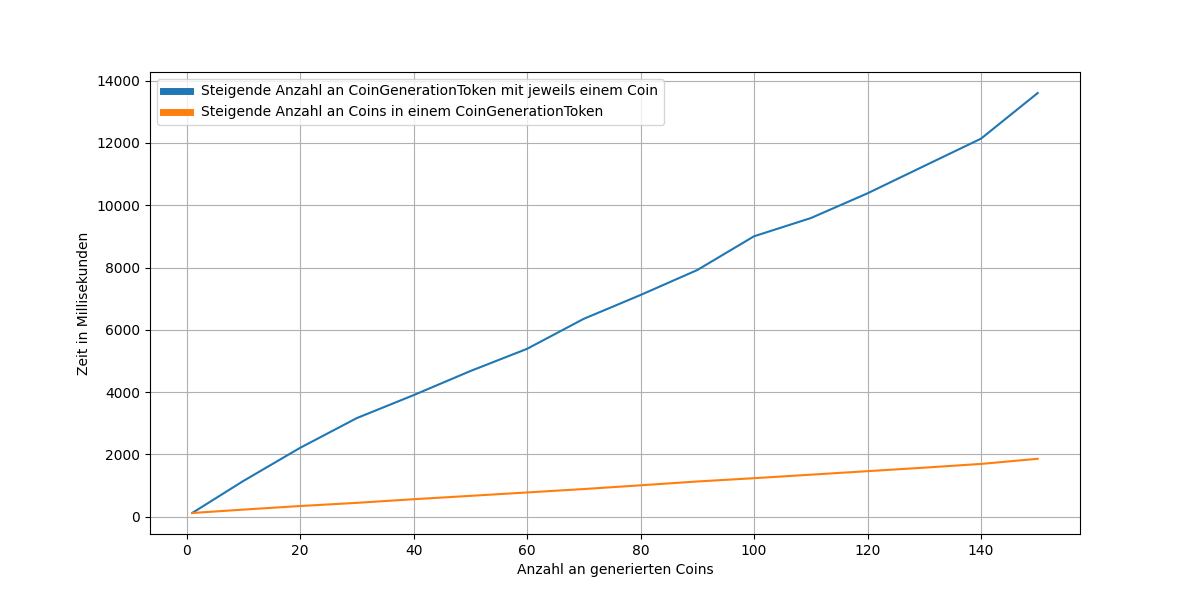
\includegraphics[width=1\textwidth]{figure_win_coins.png}
        \caption{Unterschied zwischen steigenden CoinGenerationToken und steigenden Coins innerhalb eines CoinGenerationToken auf Windows}
        \label{fig:win_coins}
    \end{subfigure}
    \hfill
    \begin{subfigure}[b]{0.49\textwidth}
        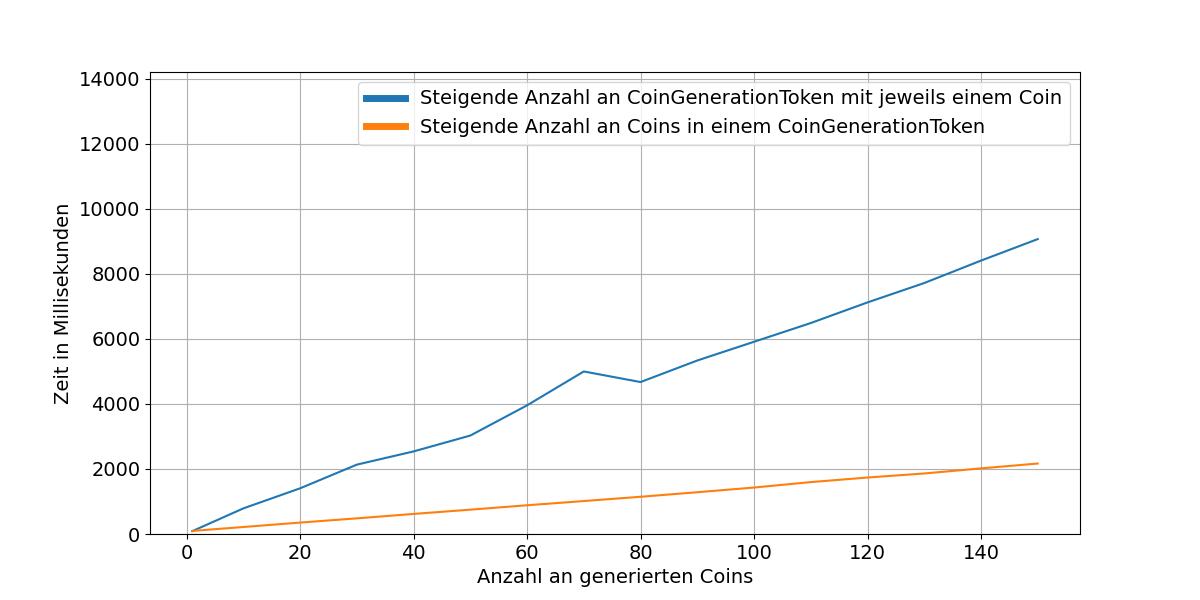
\includegraphics[width=1\textwidth]{figure_mac_coins.png}  
        \caption{Unterschied zwischen steigenden CoinGenerationToken und steigenden Coins innerhalb eines CoinGenerationToken auf MacOS}
        \label{fig:mac_coins}
    \end{subfigure}
\end{figure}

Unter direktem Vergleich der Abbildungen \ref{fig:win_coins} und \ref{fig:mac_coins} fällt auf, dass das Erstellen von einem $CoinGenerationToken$ mit 150 Coins erheblich schneller abläuft als das Erstellen von 150 \\$CoinGenerationToken$ mit jeweils einem Coin. Dies hängt mit der Nachrichtenkomplexität zusammen. In Kapitel \ref{system:coingeneration} wird beschrieben, dass für das Erstellen von Coins pro $CoinGenerationToken$ -- mit Einbezug der partiell blinden Signaturen -- sechs Kommunikationsschritte zwischen dem EX und dem DN stattfinden. Daraus ergibt sich, dass das Erstellen und Signieren von 150 Coins innerhalb eines $CoinGenerationTokens$ ebenfalls sechs Datenübertragungen umfasst, was einer Nachrichtenkomplexität von $O(6)=O(1)$ entspricht. Bei einer steigenden Anzahl $n$ an $CoinGenerationToken$ entspricht die Nachrichtenkomplexität jedoch $O(n\cdot6)=O(n)$ Datenübertragungen. Die verschlüsselten Nachrichteninhalte sind hier dafür nur $\frac{1}{150}$ Mal so groß. Der deutliche Unterschied zwischen den beiden Linien stellt eindeutig dar, dass das Signieren von 150 Coins durch einen $CoinGenerationToken$ performanter ist. Deswegen wurde in Abbildungen \ref{fig:win_3} und \ref{fig:win_4} zusätzlich die Anzahl an Coins pro $CoinGenerationToken$ erhöht, um weiterhin die nötige Menge an Coins zu erstellen und dabei die Auswirkung auf die Gesamtlaufzeit möglichst gering zu halten.

Beachtlich sind hier die unterschiedlichen Laufzeiten zwischen der Ausführung auf Windows mit einem AMD Prozessor und der Ausführung auf MacOS mit einem Intel Prozessor. Bei der Ausführung mit 150 $CoinGenerationTokens$ unterscheiden sich die Messwerte beinahe um 50\%. Auf Windows wird dafür eine Gesamtrechendauer von 13696 Millisekunden benötigt, während es auf MacOS lediglich 9277 Millisekunden sind. Gleichzeitig ist das Erstellen von 150 Coins innerhalb eines $CoinGenerationTokens$ auf Windows schneller. Dort wird eine Zeit von 1958 Millisekunden erreicht, während MacOS für die gleichen Operationen 2389 Millisekunden in Anspruch nimmt. Leider kann aufgrund des Aufbaus der beiden Computer nicht bestimmt werden, ob dieser Performanzunterschied durch das Betriebssystem oder durch den Prozessorhersteller entsteht.\\

Die folgende Abbildung \ref{fig:win_3} zeigt das Verhalten der Laufzeiten bei schrittweisem Anstieg an Datenpostfacheinträgen. Zusätzlich wurde die Anzahl an Coins pro $CoinGenerationToken$ erhöht, um ausreichend Coins bereitzustellen. Die Abbildung stellt fünf Linien dar. Sie beziehen sich auf unterschiedliche Abschnitte im Protokoll. Die blaue Linie ist die betrachtete Dauer der Coin Generierungsphase. Die orange Linie bildet die Protokollschritte 2,3 und 4 des in Kapitel \ref{system:payment} dargelegten Bezahlsystems ab. Die Schritte 5-12 sind in der grünen Linie mitinbegriffen. Die rote Linie stellt die abschließenden Schritte 13-16 dar.
\begin{figure}[H]
    \caption{Steigende Anzahl an Datenpostfacheinträgen und Coins bei einem CoinGenerationToken und einem Coin pro Bezahlung}
    \label{fig:win_3}
    \centering
    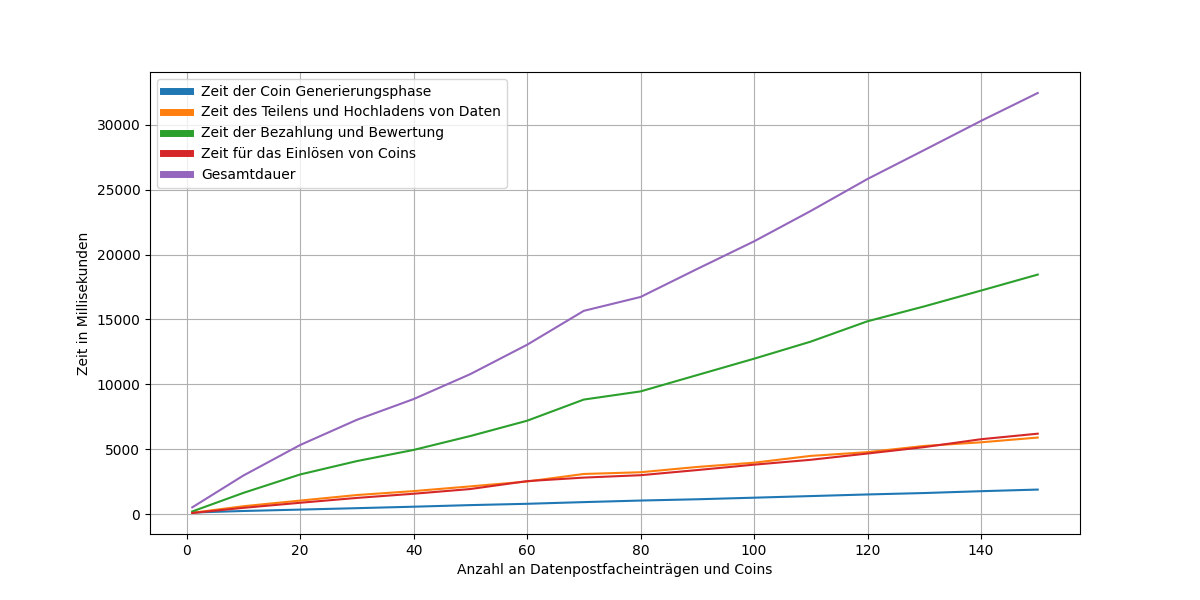
\includegraphics[width=0.8\textwidth]{figure_win_3.png}
\end{figure}
Hier ist zu sehen, dass das Teilen von 150 unterschiedlichen $DataLocations$ und $DataKeys$ in knapp unter sechs Sekunden geschieht. Verglichen mit der Zeit der Bewertung und Bezahlung ist die Zeit passend, da Protokollschritte 2 und 3 jeweils ein Mal geschehen und nur der Protokollschritt 4 \ 150 Mal ausgeführt wird. Dieser Schritt verschlüsselt die $DataLocation$, den $DataKey$, den $BewertungsToken$ und den $ReferenceCode$ symmetrisch mit MAES. Der $SHK$ wird mit Hilfe von ECC verschlüsselt.

Bei der Bezahlung und Bewertung hingegen fallen mehrere Schritt an. Hier wird für jeden Datenpostfacheintrag das erhaltene Tupel entschlüsselt, die Reputation und Daten angefragt, der Coin zur Bezahlung mit dem $ReferenceCode$ zurück an das Bezahlpostfach gesendet und der Bewertungstoken zusammen mit einer Bewertung eingereicht. Daher ist ein Anstieg von 5900 Millisekunden -- für das Hochladen von Daten -- auf 18457 Millisekunden -- für die Bearbeitung durch den DN -- beachtlich, da sich die Gesamtanzahl an Operation um ein Fünffaches erhöht.

Über die Gesamtdauer gesehen wird der erste Computer hier um 54,99\% von dem zweiten Computer unterboten. Dessen Zeiten sind in Abbildung \ref{fig:mac_3} visualisiert und liegen bei 20934 Millisekunden im Gegensatz zu 32447 Millisekunden des ersten Computers. Es ist zu erkennen, dass sich alle Zeitmessungen linear zum Anstieg des Parameters verhalten und keine polynomiellen Zeitanstiege zu erkennen sind, die die Anforderung der Skalierbarkeit verletzten würden.


\begin{figure}[H]
    \caption{Steigende Anzahl an Coins pro Bezahlung und Coins pro CoinGenerationToken bei einem Datenpostfacheintrag und CoinGenerationToken}
    \label{fig:win_4}
    \centering
    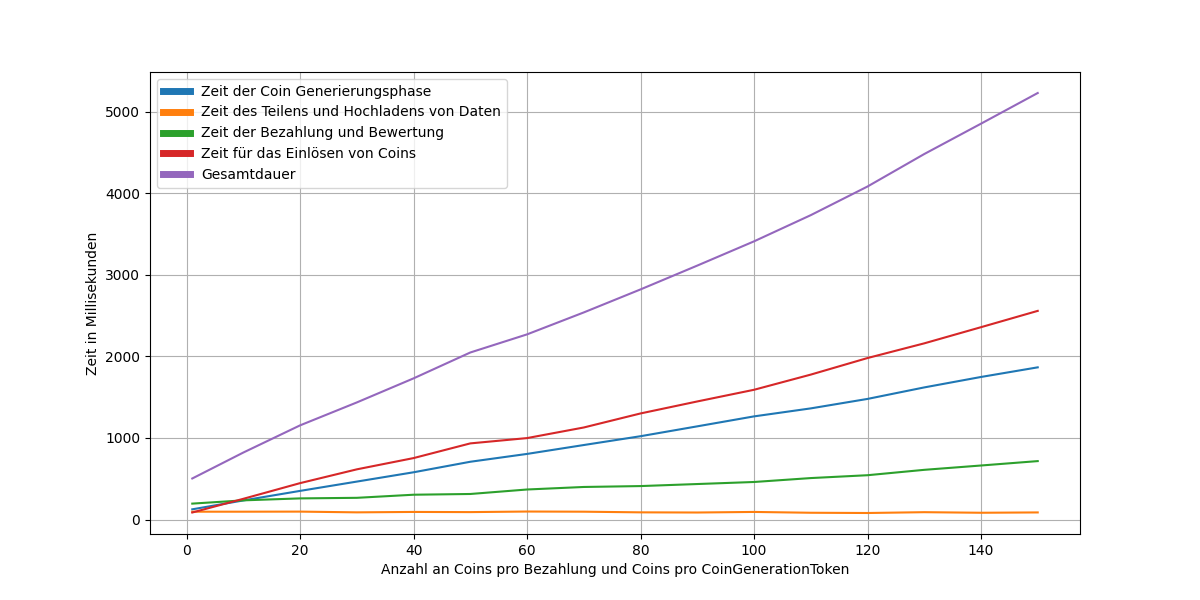
\includegraphics[width=0.8\textwidth]{figure_win_4.png}
\end{figure}
In Abbildung \ref{fig:win_4} wurde der vierte Parameter erhöht und insgesamt ein Datenpostfacheintrag mit einer steigenden Anzahl an Coins bezahlt. Die Zuteilung der Farben zu den Protokollschritten ist identisch mit der letzten Abbildung. Es wird deutlich, dass die Gesamtdauer von 32447 Millisekunden in Abbildung \ref{fig:win_3}, zu 5227 Millisekunden in Abbildung \ref{fig:win_4} sinkt. Diese Abnahme ist durch das Einsparen von hunderten Operationen begründet. Die Protokollschritte 5-12 werden nur noch ein Mal ausgeführt, anstatt jeweils 150 Mal. Dadurch sinkt die Zahl an Interaktionen zwischen dem DT und dem DN von 1200 auf 8. Im Gegenzug ist die in Schritt 12 verschlüsselte Nachricht, die sämtliche Coins zur Bezahlung beinhaltet, erheblich länger als bei der Bezahlung mit einem Coin.

Die Dauer für das Einlösen der erhaltenen Coins wird durch die verringerte Anzahl an Coinpostfacheinträgen ebenso gesenkt. Während sie in Abbildung \ref{fig:win_3} noch bei 6198 Millisekunden lag, ist sie in Abbildung \ref{fig:win_4} bereits auf 2557 Millisekunden gefallen. Dies ist auf den eingesparten Rechenaufwand durch das Entschlüsseln einer einzelnen Nachricht zurückzuführen. Die Zeit zum Erstellen und Absenden eines Datenpostfacheintrags bleibt hier konstant bei ca. 100 Millisekunden, da in jedem Durchlauf genau ein Eintrag erstellt wird und dieser nicht von der Anzahl an Coins beeinflusst wird.


\subsection{Laufzeit ohne Reputation}
\label{subsec:noRep}
Wie in Kapitel \ref{system:reputation} erwähnt wurde, kann das Anfragen der Reputation des DG sowie das Ausstellen einer Bewertung für die erhaltenen Daten übersprungen werden. Sollte ein DN keinen großen Wert auf Einhaltung der Reputationsschwelle legen oder möchte anderen DN keine Einschätzung über die Qualität liefern, so kann er den jeweiligen Schritt weglassen um Rechenaufwand zu sparen. Die Abbildung \ref{fig:win_noRep} zeigt, wie sich das Weglassen der einzelnen Schritte auf die Gesamtlaufzeit auswirkt.
Die unterschiedlich eingefärbten Teile der Balken in der Abbildung \ref{fig:win_noRep} stellen die Laufzeiten der jeweiligen Programmabschnitte dar. Für die kommenden Vergleiche wurde als Vergleichsgrundlage eine reguläre Ausführung der Protokolle gemessen. Diese reguläre Ausführung umfasst einen $CoinGenerationToken$ mit einem Coins, einen Datenpostfacheinträge und ein Coins pro Bezahlung. Diese ist in der Abbildung \ref{fig:win_noRep} auf der linken Seite zu sehen. Damit Unregelmäßigekeiten bestmöglich vermeidet werden, wurde für jeden Datensatz 50 Ausführungen gemessen und deren Durchschnitt berechnet. Die schwarzen Linien zeigen dabei die jeweils minimal und maximal Ausführungsdauer. Die Parameter werden ebenfalls in den kommenden Abschnitten \ref{subsec:runTime256Bit} und \ref{subsec:runTimeRSA} verwendet, um eine Vergleichsgrundlage zu definieren. \\
Der Balken in der Mitte verwendet die gleichen Werte und zeigt die Dauer der Ausführung, bei der das Anfragen der Reputation übersprungen wird. Eine Bewertung wird hier weiterhin abgegeben. Beim rechten Balken wird auch das Einreichen einer Bewertung übersprungen und nur eine Bezahlung abgegeben.

\begin{figure}[h]
    \caption{Laufzeitverhalten beim Überspringen der Reputationsanfrage und Bewertung}
    \label{fig:win_noRep}
    \centering
    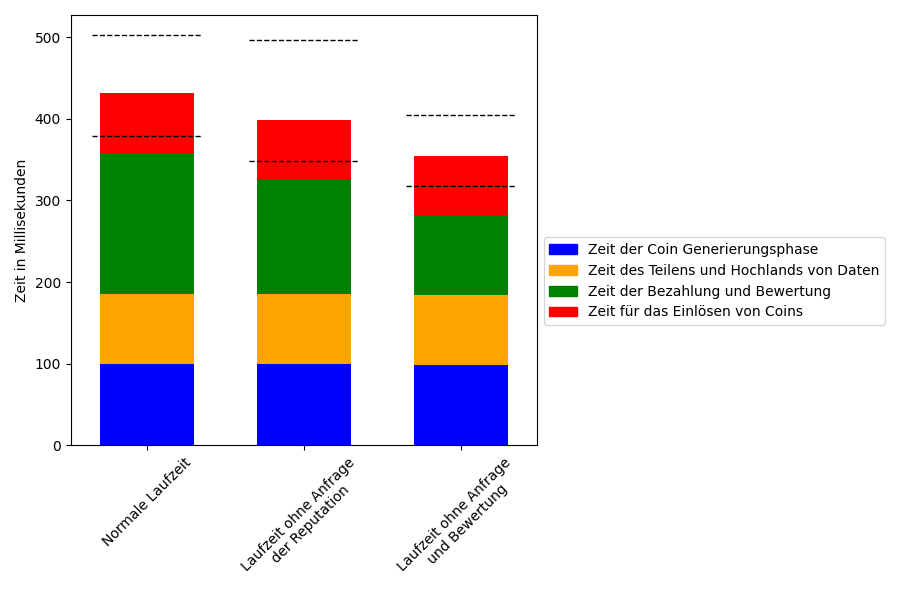
\includegraphics[width=0.8\textwidth]{figure_win_noRep_withOnlyOnes.png}
\end{figure}
In der Abbildung \ref{fig:win_noRep} ist zu erkennen, dass ein moderater Unterschied in der Ausführungsdauer entsteht, sollten die eben genannten Teile des Reputationssystems übersprungen werden. Sämtliche Zeiten -- abgesehen von der Zeit zum Bezahlen und Bewerten -- unterscheiden sich nur in Messungenauigkeiten. Durch das Entfallen der Reputationsanfrage werden bereits zwei Protokollschritte übersprungen. Der dadurch gewonnene Zeitunterschied umfasst im Durchschnitt $32,46$ Millisekunden. Beim zusätzlichen Weglassen der Bewertung ein weiterer Protokollschritt gespart. Da diese Nachricht den Bewertungstoken enthält, muss der DT beim Empfang die -- in Kapitel \ref{system:reputation} genannte -- Überprüfung vornehmen. Diese Überprüfungen bleiben beim Weglassen einer Bewertung aus, was die Laufzeit im Schnitt um weitere $44,04$ Millisekunden verkürzt. Für DN mit wenig Rechenleistung ist es daher eine Überlegung wert, die Anfrage der Reputation beispielsweise nur bei schlechten Daten durchzuführen, um zu prüfen, ob es sich um einen Betrugsversuch handelt.


\subsection{Laufzeit mit 256 Bit Security Level}
\label{subsec:runTime256Bit}
Im Kapitel \ref{chap:impl} wurde beschrieben, dass sich für die Einhaltung eines 128 Bit Security Level entschieden wurde und die Gründe dafür genannt. Der größte Nachteil ist der Anstieg der Rechenzeit, den größere Schlüssellängen mit sich ziehen. Um bewerten zu können, wie groß der dadurch entstehende Unterschied ist, wird in der Abbildung \ref{fig:win_256bit} ein Durchlauf mit 128 Bit Security Level gegen einen Durchlauf mit einem 256 Bit Security Level verglichen. Dafür behalten beide die Parameter der Vergleichsgrundlage. Das Security Bit Level von 256 Bits kann nicht ganz erreicht werden. In Abschnitt \ref{sec:aes} wird der MAES Algorithmus erklärt. Dieser ist aufgrund seines Konzeptes an einen 128 Bit Schlüssel gebunden und kann daher nicht auf 256 Bit erweitert werden. Ansonsten wurde für ECC die $secp521r1$ Kurve verwendet, die 256 Bit Sicherheit liefert \cite{ecc-duka2020elliptic}, sowie die Parameter für die partiell blinden Signaturen auf -- für 256 Bit Security übliche -- Werte angehoben. Diese entsprechen $L=15360$ und $N=512$ \cite{elaine2016recommendation}.

Die Abbildung \ref{fig:win_256bit} zeigt die gemessenen Zeitunterschiede bei der Verwendung von 256 Bit Security Parametern. Nicht in der Abbildung aufgeführt, sind die benötigten Zeiten zum Erstellen der Schlüssel, da diese beim Starten der Applikation generiert werden und daher nicht in die Berechnungszeit von Aktionen einfließen. Diese werden ein Mal zu Beginn erstellt, sind aber nicht zu vernachlässigen. Bei ECC ist der Unterschied beim Generieren eines Schlüssels vergleichsweise gering. Die Kurven $secp256k1$ und $secp521r1$ unterscheiden sich hierbei um circa 10 Millisekunden \cite{ecc-duka2020elliptic}. Das Generieren von Parametern der partiell blinden Signaturen hingegen unterscheidet sich in der eigenen Implementation signifikant. Für den Vergleich wurde die Zeit der Generierung für 128 Bit und 256 Bit jeweils 10 Mal gemessen. Die Werte für 128 Bit lagen zwischen 95 - 6737 Millisekunden mit einem Durchschnitt von 1760 Millisekunden. Bei 256 Bit hingegen lagen die Werte zwischen 6556 - 102644 Millisekunden mit einem Durchschnittswert von 38022 Millisekunden. Hier ist der Unterschied zwischen den Security Leveln deutlich erkennbar.

\begin{figure}[h]
    \caption{Laufzeitverhalten unter Verwendung eines 256 Bit Security Levels}
    \label{fig:win_256bit}
    \centering
    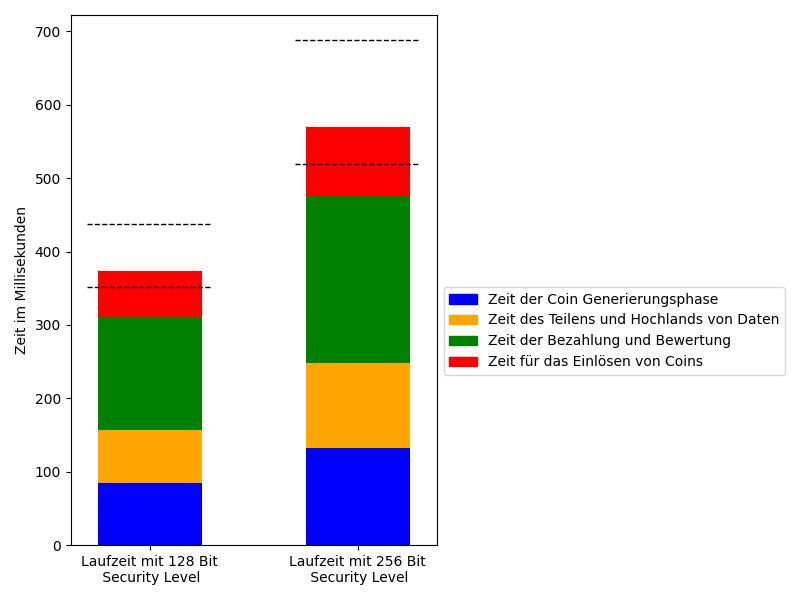
\includegraphics[width=0.7\textwidth]{figure_win_256Bit_withOnlyOnes.png}
\end{figure}
Die durch das Verschlüsseln sowie Signieren von Nachrichten entstehenden Zeitunterschiede, sind in Abbilung \ref{fig:win_256bit} dargestellt. Für die Werterhebung wurde ein Durchlauf mit den Vergleichsparametern aus \ref{subsec:noRep} für 128 Bit auf der linken Seiten und 256 Bit auf der rechten Seite ausgeführt. Hier sind die unterschiedlichen Laufzeiten gut zu erkennen. Wieder gilt, dass 50 Ausführung gemessen wurden, von welchen der Durchschnitt durch den Balken und die Minimal- und Maximallaufzeit durch die schwarzen Linien dargestellt sind. Die Gesamtausführungszeit steigt durchschnittlich um $32,18\%$, von $432,6$ Millisekunden auf $571,47$ Millisekunden. Da alle Protokollschritte Daten verschlüsselt übertragen, sind Anstiege in allen Bereichen zu verzeichnen. Diese Anstiege sind in allen Protokollphase ähnlich. Bei der Coin Generierungsphase wächst die gemessene Zeit am stärksten -- um $34,16\%$, von $99,06$ auf $133,9$ Millisekunden. Dies hängt mit der Anwendung der partiell blinden Signatur zusammen, die durch den erheblich längeren Schlüssel etwas mehr Zeit in Anspruch nimmt als das Verschlüsseln mit einem doppelt so langen ECC Schlüssel. Die Auswirkung der Schlüsselgröße --von partiell blinden Signaturen -- sind beim Signieren von einem Coin jedoch vergleichsweise gering, da hier der Verschlüsselungsaufwand hauptsächlich bei der Datenübertragungen entsteht. Sollten beispielsweise 100 Coins signiert werden, hätte die Schlüssellänge größere Auswirkungen.

Das Erstellen und Hochladen der eines Datenpostfacheinträge verzögert sich um $29,17$ Millisekunden und liegt unter Verwendung von 256 Bit bei insgesamt $115,23$ Millisekunden. Die Steigerung liegt hier -- dicht hinter der Coin Generierungsphase -- bei $33,9\%$. Die Zeit zum Bezahlen steigt von $172,96$ auf $227,13$ Millisekunden -- um $31,32\%$. Die Zeit zum Einlösen der Coins steigert sich am geringsten. Der gemessene Anstieg beträgt hier $21,84$ Millisekunden, was $29,98\%$ entspricht. Da sich die Funktionsweise der partiell blinden Signaturen stark mit der von RSA ähnelt, kann die kleine Laufzeitsteigerung mit den geringen Validierungszeiten von RSA Signaturen \cite{rsa-Singh2016Performance} in Verbindung gebracht werden.

\subsection{Laufzeit mit RSA}
\label{subsec:runTimeRSA}
In Abschnitt \ref{sec:ecc} wird erklärt, dass die elliptische Kurven Kryptographie große Unterschiede in der Laufzeit im Vergleich zu RSA erzielen kann. Für eine Bewertung des Zeitaufwands, der durch die Verwendung von ECC gewonnen wird, wurden sämtliche ECC Kommunikationsverschlüsselungen durch RSA ersetzt und die Zeit einer Ausführung gemessen. Für die RSA Schlüssel wurde eine Länge von 3072 Bit verwendet, so wie sie in der Literatur für ein Bit Security Level von 128 Bit empfohlen wird \cite{elaine2016recommendation}. Die daraus entstandenen Ergebnisse sind in Abbilung \ref{fig:win_rsa} zu sehen. Sie zeigen die Ausführung mit den Kontrollparametern, unter Verwendung von ECC auf der linken Seite und Verwendung von RSA auf der rechten Seite. 

\begin{figure}[h]
    \caption{Laufzeitverhalten unter Verwendung von RSA für Verschlüsselung}
    \label{fig:win_rsa}
    \centering
    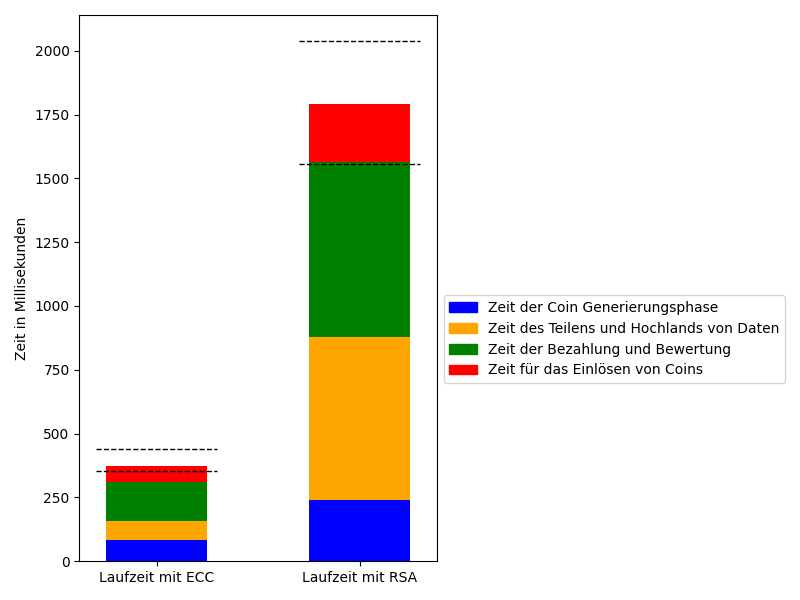
\includegraphics[width=0.7\textwidth]{figure_win_RSA_withOnlyOnes.png}
\end{figure}
Die hier entstehenden Unterschiede sind deutlich erkennbar. Durch die Verwendung von RSA erhöht sich die durchschnittliche Gesamtlaufzeit um $383,92\%$. Dabei wird die Zeit für das Teilen von Daten langsamer als die anderen Protokollschritte. Sie steigt im Schnitt um $597,77\%$ von $86,06$ auf $514,44$ Millisekunden. Dass hier so ein großer Laufzeitunterschied zu verzeichnen ist, hängt damit zusammen, dass der DG die Liste an Aufrufen entschlüsseln muss. Diese ist die längste Nachricht innerhalb aller Protokolle. Da das entschlüsseln mit RSA den zeitaufwändigen Teil der Berechnung ausmacht \cite{ecc-mahto2018performance}, ist dieses Verhalten nachvollziehbar. Die nächste größte Veränderung liegt bei $390,22\%$ bei der Zeit für das Bezahlen und Bewerten. Dicht gefolgt von der Zeit für das Einlösen der Coins. Diese erhöht sich um $319,85\%$ von $72,86$ auf $233,04$ Millisekunden. Die Zeit der Coin Generierungsphase steigert sich um $239,11\%$. Anhand der Abbildung \ref{fig:win_rsa} ist eindeutig erkennbar, dass die Verwendung von ECC als Verschlüsselungsmethode große Laufzeitunterschiede liefert. Daher wird die Verwendung von ECC hier eindeutig vor RSA bevorzugt.

Abschließend kann zusammengefasst werden, dass sich die Rechendauer der vier verschiedenen Protokollabschnitte mit einer steigenden Anzahl an Eingaben linear verhält. Zwar laufen einige Abschnitte schneller als andere, wie beispielsweise das Erstellen von Coins durch einen $CoinGenerationToken$ anstatt durch mehrere, was sich selbst von Computer zu Computer unterschiedlich verhalten kann. Allerdings wird zu keinem Zeitpunkt ein polynomielles Laufzeitverhalten beobachtet. Das Überspringen von Reputationsanfragen, wie das Prüfen der Reputation oder das Einreichen einer Bewertung, ist in bestimmten Situationen möglich und liefert dabei Laufzeiteinsparungen von bis zu über 70 Millisekunden pro Bezahlvorgang. Daher können Strategien entwickelt werden, um die Verwendung dieser Anfragen zu minimieren und so den Rechenaufwand zu verringern. Insbesondere für DN, die nur über eingeschränkte Rechenleistung verfügen, sind solche Möglichkeiten in Betracht zu ziehen. Ein Security Bit Level von 128 Bit ist laut Literatur auch für die kommenden Jahre mehr als ausreichend \cite{elaine2016recommendation,bsi2020cryptographic}. Während der Umstieg auf ein Security Bit Level von 256 Bits, in anbetracht der sensiblen kommunizierten Daten nachvollziehbar wäre, zieht dieser einen zusätzlichen Rechenaufwand mit sich. Die dadurch hinzukommende Steigerung von einem Drittel ist nicht zu vernachlässigen. Aufgrund dessen wird für die Verwendung des Systems ein Security Bit Level von 128 Bit empfohlen. Anhand der in Abbildung \ref{fig:win_rsa} visualisierten Performanzunterschiede zwischen ECC und RSA wird hier eindeutig ECC für die Verschlüsselung und Schlüsselgenerierung empfohlen, da es RSA beinah um das vierfache überholt.

\section{Erfüllen der Anforderungen}
In diesem Abschnitt wird erläutert, dass alle der in Kapitel \ref{chap:req} gesetzten Anforderungen durch das hier präsentierte Konzept erfüllt werden.

\paragraph{Funktionale Anforderungen.}
\begin{enumerate}
    \item Die Präsenz eines Bezahlsystems ist eindeutig. Durch die Coin Generierungsphase wird zusammen mit den Protokollschritten 11,14,15 und 17 des Bezahlsystems aus Kapitel \ref{system:payment} ein Austausch von Zahlungsmitteln ermöglicht, der den DG für seine Daten entlohnt.
    \item Es existiert ein Reputationswert. Dieser wird zwar nicht durch den DN für jeden DG evaluiert, allerdings wird durch die Angabe des Reputationsschwellwertes, beim Erstellen eines Aufrufs sichergestellt, dass ein DN eine gewisse Qualität vorraussetzen kann.
    \item Die Streitfälle \textit{Fehlerhafte Coins} sowie \textit{Bezahlzeitraum überschritten} sorgen dafür, dass ein DG bei rechtmäßiger Bereitstellung seiner Daten eine Bezahlung erhält. Der $SHK$ kann dabei verwendet werden, um die Übertragung der Coins zu beweisen.
    \item Der Bewertungstoken, der Teil des Datenpostfacheintrags ist, liefert dem DN die Möglichkeit, eine Bewertung der Daten an den DT zu senden, ohne dabei die Identität des DG zu kennen.
    \item Sollte ein DG versuchen, eine Bewertung seiner Daten zu verhindern, so greifen die Streitfälle \textit{Kein/Doppleter Bewertungstoken} oder \textit{Inkorrekte Signatur}, die den DG bestrafen.
    \item Durch den $nonce$, der Teil des Bewertungstokens ist, wird sichergestellt, dass ein DN nur eine Bewertung pro Token und damit auch pro Handel abgeben kann.
\end{enumerate} 

\paragraph{Nicht funktionale Anforderungen.}
\begin{enumerate}
    \item Die Betrachtung der Angreifermodelle aus den Abschnitten \ref{subsec:adversaryCoinGen}, \ref{subsec:adversaryPayment} und \ref{subsec:adversaryRep} zeigen, dass der DG und dessen Verhalten zu keinem Zeitpunkt des Protokolls bestimmt werden können. Er bleibt daher anonym.
    \item Die Unverkettbarkeit wird ebenfalls in den Angreifermodellen gezeigt. Durch die Funktionsweise bleiben sowohl verschiedene Handel eines DG, als auch die Beziehung zwischen DG und DN unverkettbar.
    \item In dem Abschnitt \ref{sec:computationTime} wird gezeigt, dass eine Transkationen von Daten im Tausch für Coins sowie das Einlösen dieser Coins, in unter einer Sekunde abläuft, was in diesem Kontext -- vorallem verglichen mit Alternativen wie Bitcoin -- vernachlässigbar ist.
    \item Abschnitt \ref{sec:computationTime} zeigt zusätzlich, dass der Rechenaufwand mit steigender Anzahl an Transkationen linear steigt.
    \item In Abschnitt \ref{sec:auswertungSecurity} wird dargelegt, dass das System die Vertraulichkeit und Integrität der Daten und Coins beim Austausch dieser schützt.
\end{enumerate}

Es sind sowohl alle funktionalen, als auch nicht funktionalen Anforderungen an das System erfüllt.

\section{Beantwortung der Forschungsfragen}
In der Einleitung in Kapitel \ref{chap:intro} wurden zwei Forschungsfragen genannt, die in den folgenden Abschnitten beantwortet werden.

\subsection{Wie kann ein privatsphäreschützender Anreiz zur Benutzung eines Datentreuhandmodells geschaffen werden?}
Datentreuhandsysteme stellen einen großen Schritt bei der fairen und transparenten Kommunikation von Daten dar. Das Konzept birgt viel Potential für die zukünftige Entwicklung und Innovation. Allerdings gibt es für Privatpersonen aktuell wenige Anreize, die Benutzung eines Datentreuhandsystems in betracht zu ziehen. Das in dieser Bachelorarbeit vorgestellte Anreizsystem legt vorallem großen Wert auf die Anonymität des DG, da dieser bei vielen Customer to Business Datentreuhandsystemen im Vordergrund steht. Die Wahl von Geld als Anreiz ist aufgrund der in Abschnitt \ref{sec:incentiveExplaination} genannten Punkte nachvollziehbar. Nachdem einige verwandte Arbeiten mit Bezug auf anonymen Geldtransfer zwischen zwei Parteien untersucht wurden, wurde deutlich, dass keine dieser Arbeiten alle Anforderungen abdeckt. Deswegen wurde in Kapitel \ref{chap:systems} ein neues Bezahlsystem entworfen, dass für die Verwendung innerhalb eines Datentreuhändermodells genutzt werden kann und alle Anforderungen erfüllt. Es bietet Spielräume um die Implementation dem jeweiligen Anwendungsfall anzupassen. Im Anschluss wurde geschildert, dass sowohl das Bezahlsystem, als auch das dazugehörige Coin Generierungssystem gegen diverse verschiedene Angreifer sicher sind und Laufzeiten von unter einer halben Sekunde für einen vollständigen Durchlauf benötigen. Das Laufzeitverhalten der Systeme wurde unter anderem mit steigenden Parameterzahlen, sowie unter der Verwendung verschiedener Verschlüsselungsmethoden und Sicherheitsniveaus beobachtet. Insgesamt liefert das in dieser Bachelorarbeit präsentierte Anreizsystem eine privatsphäreschützende Methode um Privatpersonen für den Gebrauch eines Datentreuhänders zu belohnen.

\subsection{Wie kann dieser Anreiz gegen Missbrauch geschützt werden?}
Damit dieser finanzielle Anreiz nicht schutzlos durch bösartige Individuen ausgenutzt werden kann, wurden in dieser Bachelorarbeit zwei Methoden verwendet, um eine unrechtmäßige Verwendung festzustellen. Die erste Methode umfasst ein Streitfallsystem, in dem für eine gegebene Interaktion zwischen DG und DN -- in der sich einer der beiden Akteure betrogen fühlt -- der Datentreuhänder als Streitschlichter eingesetzt werden kann. Er erhält ausschließlich die Einsicht in die -- in der Kommunikation übertragenen -- Daten und kann als neutrale Instanz entscheiden, ob bei dem Handel ein Betrug durch einen der beiden Akteure vorliegt. Die zweite Methode ist die Verwendung eines Reputationssystems. Hierfür wurden ebenfalls verwandte Arbeiten betrachtet und festgestellt, dass keine dieser die nötigen Anforderungen erfüllt. Deswegen wurde in Kapitel \ref{system:reputation} ein neues Reputationssystem entworfen, dass jedem DG einen Rufwert zuordnet. Er kann durch die Bewertung von DNs nach oben oder unten bewegt werden und spiegelt die Vertrauenswürdigkeit eines DGs wieder. Durch diese beiden Methoden wird das System vor Missbrauch des Anreizes geschützt.
\section{Diskussion}
\label{sec:discussion}
In diesem Abschnitt werden einige offene Punkte genannt, die bei der Entwicklung der Konzepte entstanden sind, aber noch nicht umgesetzt werden konnten. 

Der erste Punkt ist die saubere Umsetzung der Qualitätsbewertung durch den DT. In Kapitel \ref{sec:dt} wird beschrieben, dass manche DT Mechanismen zur Qualitätssicherung besitzen. Sollte das System jedoch in einem DT-System implementiert werden, das nicht über solch einen Mechanismus verfügt, kann die Qualität nicht bewertet werden, was eine große Angriffsmöglichkeit für bösartige DG schafft. Zusätzlich werden bei der Schlichtung eines Streitfalls viele Informationen für den DT einsehbar. All diese Informationen sind zum Schlichten des Streitfalls erforderlich, weshalb sie nicht privat gehalten werden können. Trotzdem kann ein Ziel von zukünftigen Arbeiten sein, die Menge an Informationen, die beim Schlichten eines Streitfalls preisgegeben werden, zu minimieren.

Der nächste Punkt ist die Verwendung des DN Zertifikats. Es führt zu einer großen Schwachstelle, sollte ein DN sein Zertifikat öffentlich machen. Da es keine Informationen über den DN beinhaltet, könnte ein DG der in Besitz eines solchen Zertifikates gelangt, sich selbst Bewertungen ausstellen. Deswegen sollte -- bevor das System produktiv eingesetzt wird -- die Verwendung des Zertifikates durch eine andere Art von Zero Knowledge Proof ersetzt werden. Dieser Schritt wurde hier aus zeitlichen Gründen ausgelassen.

Zuletzt war ein alternativer Ansatz für die Umsetzung des Reputationssystems angedacht. Hier wird begründet, warum der aktuelle dem alternativen Ansatz bevorzugt wird. Der alternative Ansatz basiert auf einem Beweis von erhaltenen Coins. Hier wird beim Einlösen von Coins durch den EX ein Zertifikat ausgestellt, dass belegt, dass der DG erfolgreich eine Summe an Coins eingelöst hat. Dieses Zertifikat kann anstatt des Reputationswertes dem DN vorgelegt werden, um den Rufwert eines DG zu zeigen. Da ein hoher Betrag eines DG von einer langen erfolgreichen Benutzung des DT zeugt, kann einem DG mit hoher Summe mehr vertraut werden. \\
Dieser Ansatz hat jedoch zwei Schwachstellen. Zuerst kann ein solches Zertifikat leicht gestohlen werden. Da es keine Informationen über den Inhaber enthalten darf -- da sonst die Anonymität des DG gegenüber des DN nicht mehr gewährleistet ist -- kann es durch einen Dieb als dessen eigenes Zertifikat verwendet werden. Die zweite Schwachstelle ist, dass ein DG mit hohem Betrag auf seinem Zertifikat nicht mehr dazu angereizt, qualitativ hochweritge Daten zu liefern. Da sich die Menge der erhaltenen Coins nicht verkleinern kann, kann er konstant qualitativ schlechte Daten verkaufen ohne dass dies Auswirkungen auf seinen Ruf hat. Aus diesen Gründen fiel die Entscheidung  auf eine reputationswertbasierte Variante.
% länge des ciphertext lässt schließen wie viele coins übertragen werden

%==================================================================================================


\chapter{Zusammenfassung}
Durch die neutrale Kontrolle bieten Datentreuhandmodelle ein großes Potential für zukünftige Entwicklung. Mit den bereits bestehenden Anwendungsfällen wird Innovation in den unterschiedlichsten Bereichen von Logistik bis hin zur personenbezogenen Datenverwaltung ermöglicht. Allerdings gibt es aktuell kaum Anreize für Privatpersonen zur Benutzung eines Customer to Business DTs. Deswegen wurden in dieser Bachelorarbeit mehrere zusammenhängende Systeme entworfen, die eine finanzielle Entlohnung für das Teilen von Daten in Aussicht stellen. Die zu Beginn in Kapitel \ref{chap:req} dargelegten Angreifermodelle verdeutlichen alle möglichen Angriffsakteure, gegen die die Systeme gerüstet sein müssen und geben gleichzeitig eine Liste an Anforderungen vor. Die Liste wird durch Schutzziele von C2B Datentreuhandmodellen -- wie beispielsweise das Schützen der Identität des DG -- erweitert. Daraufhin wurden einige verwandte Arbeiten in dem Gebiet der anonymen Bezahlsysteme analysiert. Keine der betrachteten Arbeiten konnte jedoch alle Anforderungen erfüllen. Ein neues Bezahlsystem musste daher entworfen werden, dass den Anforderungen gerecht wird. Der Entwurf übernimmt einige Designentscheidungen von GNU Taler und Privacy Pass, wie die Signierphase, in der Coins erstellt und von dem EX blind signiert werden. Die Systeme erlauben es einem DG seine Daten hochzuladen und den Zugang zu diesen Daten verschlüsselt und anonym an DNs weiterzuleiten. Ein DN kann die Daten auswerten und ist im Anschluss dazu verpflichtet, dem DG eine vorher vereinbarte Mengean Geld zu senden. Der DG kann diese anonym abrufen und bei einem EX auf einem bevorzugten Zahlungsweg auszahlen lassen.

Um möglichen Missbrauch der Systeme vorzubeugen, wurden zwei Mechanismen zum Erkennen von Betrug in die Systemarchitektur eingebaut. Der erste Mechanismus ist ein Streitfallsystem. Da sowohl DG als auch DN betrügerische Intentionen verfolgen können, werden die wichtigen Informationen -- wie Datenzugang und Coins -- mit einem symmetrischen Schlüssel verschlüsselt über den beide Handelspartner verfügen. Sollte sich einer der beiden in dem Handel betrogen fühlen, kann er diesen symmetrischen Schlüssel an den DT senden. Da sämtliche Kommunikation über den DT abgewickelt und gespeichert wird, ist er nicht auf die Aussage einer der Parteien angewiesen, sondern kann die initial übertragenen Nachrichten entschlüsseln. Je nach erhobenem Streitfall, kann der DT die vorliegenden Informationen analysieren und neutral entscheiden, ob einer der Parteien versucht hat zu betrügen.

Der zweite Mechanismus der vor Missbrauch schützt, wird durch die Einbettung eines Reputationssystems dargestellt. Jeder DG besitzt dafür eine Reputation, die bestimmt auf welche Aufrufe er Zugriff besitzt. Sollte ein DN für einen Aufruf ausschließlich qualitativ hochweritge Daten benötigen, so kann er einen hohen Reputationsschwellwert beim Erstellen eines Aufrufs angeben. Daraus folgt, dass nur DG mit einer ausreichend hohen Reputationswerten, Einsicht auf den Aufruf erhalten und ihre Daten mit dem DN teilen können. Dabei kann der DN nicht bestimmen, für wen er die Bewertung ausstellt. Nur der DT kann bei Erhalt der Bewertung herausfinden, welchem DG die Bewertung zuzuordnen ist. Da auch dieses System anfällig für Betrug ist, wurden die Streitfallszenarien auf mögliche Betrugsversuche innerhalb des Reputationssystems erweitert. 

Abschnitt \ref{sec:auswertungSecurity} zeigt die Sicherheit der drei Systeme (Coingenerierung, Bezahlung, Bewertung) anhand der zu Beginn definierten Angreifermodelle. Während die Angreifermodelle in Kapitel \ref{chap:req} noch grob formuliert waren, wurden diese in Kapitel \ref{chap:auswertung} präziser. Alle drei Systeme zeigten dabei eine hohe Resistenz gegen die unterschiedlichen Angreifer und verschiedene Angriffsmethoden.

In Abschnitt \ref{sec:computationTime} wurde die Laufzeiten der Systeme mit steigenden Parametern untersucht. Dabei wurde ein lineares Wachstum bei jedem der einzelnen Parameter beobachtet, wodurch die Anforderung der Skalierbarkeit erfüllt wurde. In dem Abschnitt wurden zusätzlich Vergleiche der Laufzeit unter andern Bedingung erhoben. Der erste Vergleich bezog sich auf den zeitlichen Unterschied beim Überspringen der Reputationsprüfung und Bewertung. Da diese beiden Schritte nur vor Betrug schützen sollen, können sie optional ausgelassen werden um Rechenaufwand zu sparen. Dabei ergab sich ein Zeitersparnis von knapp 20\%. Für den nächsten Vergleich wurde das in der Implementation verwendete Bit Security Level von 128 Bits auf 256 Bits erhöht. Dabei ergab sich eine Steigerung von ungefähr einem Drittel. Der dritte Vergleich ersetzt die vorgeschlagene elliptische Kurven Kryptographie durch den weit verbreiteten RSA Algorithmus. Der Tausch der Verschlüsselungsmethode erhöhte die Laufzeit um circa 390\%.

Die hier entworfenen Systeme werden ihren Anforderungen und Zielen gerecht. Sie liefern einen idealen Anreiz für Privatpersonen, sich für die Verwendung eines Datentreuhandmodell zu öffnen und schützen dabei vor Missbrauch durch Privatpersonen und Firmen oder Forschungseinrichtungen. Und während wenige in Abschnitt \ref{sec:discussion} angesprochene Aspekte offen bleiben, sind die in der Einleitung gestellten Forschungsfragen durch die System beantwortet.


%==================================================================================================

\newpage

\thispagestyle{empty}

\vspace*{\fill}
\pagestyle{empty}

{
    \normalsize
    \begin{center}
        \textbf{Eidesstattliche Erklärung}
    \end{center}
    Hiermit versichere ich an Eides statt, dass ich die vorliegende Arbeit im Bachelorstudiengang Software-System-Entwicklung
    selbstständig verfasst und keine anderen als die angegebenen Hilfsmittel –- insbesondere keine im Quellenverzeichnis nicht benannten Internet-Quellen –- benutzt habe. Alle Stellen, die wörtlich oder sinngemäß aus Veröffentlichungen entnommen wurden, sind als solche kenntlich gemacht. Ich versichere weiterhin, dass ich die Arbeit vorher nicht in einem anderen Prüfungsverfahren eingereicht habe.
    \vspace*{1cm}\\
    Hamburg, den \today
    \hspace*{\fill}\begin{tabular}{@{}l@{}}\hline
    \makebox[5cm]{Knut Hoffmeister}
    \end{tabular}
    \vspace*{3cm}
}
\vspace*{\fill}

\printbibliography

\appendix 
\chapter{Laufzeit Abbildungen}
\begin{figure}[H]
    \caption{Steigende Anzahl an Datenpostfacheinträgen und Coins bei einem CoinGenerationToken und einem Coin pro Bezahlung auf MacOs}
    \centering
    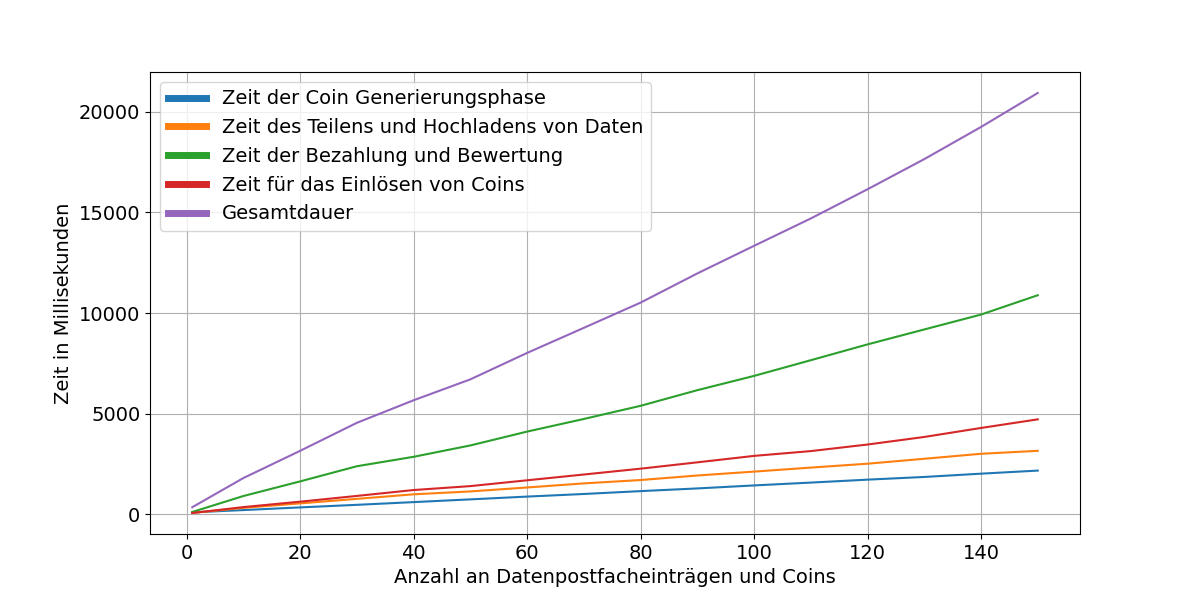
\includegraphics[width=0.8\textwidth]{figure_mac_3.png}
    \label{fig:mac_3}
\end{figure}
\begin{figure}[H]
    \caption{Steigende Anzahl an Coins pro Bezahlung und Coins pro CoinGenerationToken bei einem Datenpostfacheintrag und CoinGenerationToken auf MacOs}
    \centering
    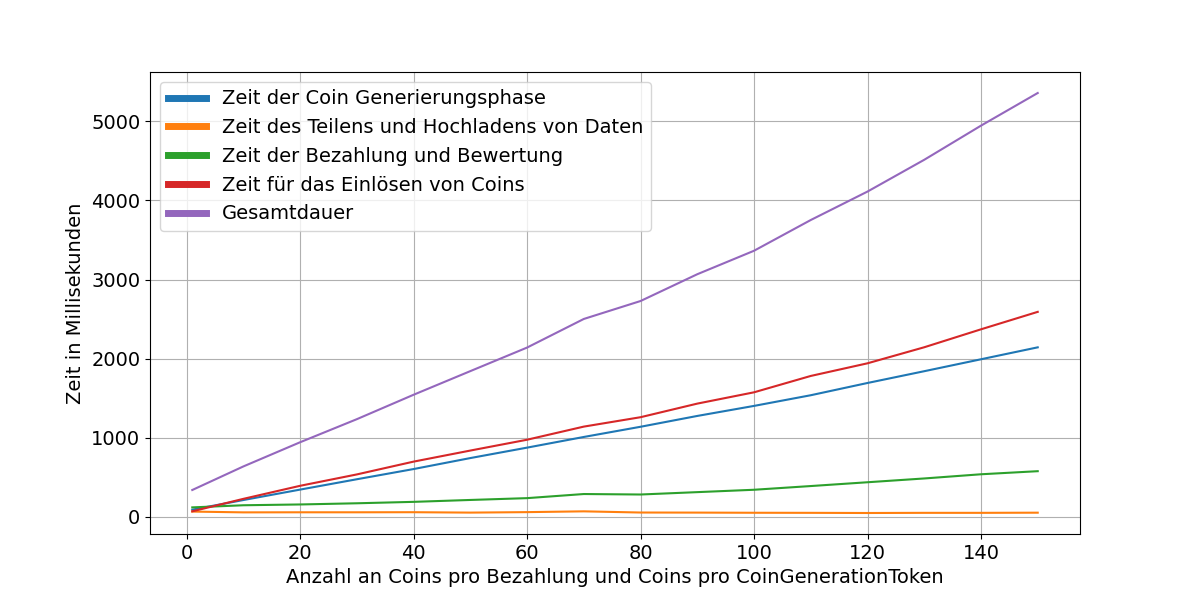
\includegraphics[width=0.8\textwidth]{figure_mac_4.png}
    \label{fig:mac_4}
\end{figure}
\end{document}